\chapter{Implementation}

\section{AI Model}

As mentioned in Chapter 3, \texttt{ChatGPT-3.5 Turbo} was chosen as the main AI model for converting legal employment contracts into Solidity code. To train it, two datasets are required: one for training and the other for validation. One problem encountered was the absence of pre-existing datasets for this specific task, as no prior attempts to address this conversion process were found in existing literature or online resources. Consequently, the only solution was to create a custom dataset manually. This dataset should include pairs of documents:  each containing a legal employment contract alongside its corresponding smart contract. To grasp the structure of these contracts, an analysis of a general-purpose smart contract developed will be done first. % Or "To understand the structure of these contracts, we will first examine the general-purpose smart contract developed." %

\subsection{General Purpose Smart Contract}

As discussed in the previous chapter, the decision was made to delegate the counting of job performance metrics to the backend. This avoids the high costs of doing it within the smart contract. The main job of the smart contract is to securely hold funds and manage the employment contract transparently, helping employers and employees interact smoothly. Here is the implementation of a general-purpose smart contract:

\begin{lstlisting}[caption=General Purpose Smart Contract]
// SPDX-License-Identifier: MIT
pragma solidity ^0.8.0;

import "node_modules/@openzeppelin/contracts/token/ERC20/IERC20.sol"; // Interface for ERC20 tokens
import "node_modules/@openzeppelin/contracts/utils/ReentrancyGuard.sol"; // Prevent re-entrancy attacks

contract EmploymentContract is ReentrancyGuard {
    address public employer;
    address public employee = 0x2df1c51e09aecf9cacb7bc98cb1742757f163df7;
    address private authorisedApp; // Address of the authorised app to update metrics
    uint256 public salary; // Monthly salary amount in USDC
    IERC20 private usdcToken; // USDC token contract interface
    uint256 public startDate; // Converted to unix
    uint256 public terminationDate; // Converted to unix
    uint256 public lastSalaryPaidDate; // Tracks last salary payment date
    uint256 public performanceScore; // Performance score, updated by the authorised app
    uint256 public performanceThreshold;
    bool public isEmployed; // Employment status
    string public salaryType; // How often a salary payment to be initiated

    event SalaryUpdated(uint256 newSalary);
    event BonusPaid(uint256 bonusAmount);
    event EmploymentTerminated(string message);
    event DisputeResolved(string message);
    event SalaryPaid(uint256 amount);
    event PerformanceScoreUpdated(uint256 score);
    event PerformanceThresholdUpdated(uint256 threshold);
    event TerminationDateUpdated(uint256 newTerminationDate);

    modifier onlyAuthorisedApp() {
        require(msg.sender == authorisedApp, "Caller is not the authorised app");
        _;
    }

    constructor(
        address _authorisedApp,
        address _usdcTokenAddress
    ) {
        employer = msg.sender; // The address deploying the contract is the employer
        authorisedApp = _authorisedApp;
        usdcToken = IERC20(_usdcTokenAddress);
        lastSalaryPaidDate = startDate; // Initialise with start date
    }

      // Function to check contract balance (for employer's view)
    function checkContractBalance() external view returns (uint256) {
        return usdcToken.balanceOf(address(this));
    }

    // Function to deposit USDC into the contract for salary payments
    function depositSalaryFunds(uint256 _amount) external nonReentrant {
        require(msg.sender == employer, "Only the employer can deposit funds");
        usdcToken.transferFrom(msg.sender, address(this), _amount);
    }

    // Function to automatically withdraw monthly salary funds from the employer
    function monthlyFunding() external onlyAuthorisedApp nonReentrant {
        uint256 amountNeeded = salary * 3; // Ensure buffer for 3 months
        uint256 currentBalance = usdcToken.balanceOf(address(this));
        uint256 shortfall = 0;

        if (currentBalance < amountNeeded) {
            shortfall = amountNeeded - currentBalance;
            // Attempt to transfer the shortfall from the employer to the contract
            usdcToken.transferFrom(employer, address(this), shortfall);
        }
    }

    // Automatically pay salary on a monthly basis
    function autoPaySalary() external onlyAuthorisedApp nonReentrant {
        require(isEmployed, "Employment has ended");
        require(block.timestamp >= lastSalaryPaidDate + 30 days, "Salary already paid for this month");
        require(usdcToken.balanceOf(address(this)) >= salary, "Insufficient funds in contract");
        require(performanceScore >= performanceThreshold, "Performance score does not meet the required threshold. Employee is underperforming");

        lastSalaryPaidDate += 30 days; // Update last salary paid date to current month
        usdcToken.transfer(employee, salary);
        emit SalaryPaid(salary);
    }

    // Update performance score
    function updatePerformanceScore(uint256 _newScore) external onlyAuthorisedApp {
        performanceScore = _newScore;
        emit PerformanceScoreUpdated(_newScore);
    }

    function updatePerformanceThreshold(uint256 _threshold) external onlyAuthorisedApp {
        performanceThreshold = _threshold;
        emit PerformanceThresholdUpdated(_threshold);
    }

    // Extend employment termination date
    function extendTerminationDate(uint256 _newTerminationDate) external onlyAuthorisedApp {
        require(_newTerminationDate > terminationDate, "New date must be after current termination date");
        terminationDate = _newTerminationDate;
        emit TerminationDateUpdated(_newTerminationDate);
    }

    // Update salary
    function updateSalary(uint256 _newSalary) external onlyAuthorisedApp {
        salary = _newSalary;
        emit SalaryUpdated(_newSalary);
    }

    // Pay bonus
    function payBonus(uint256 _bonusAmount) external onlyAuthorisedApp nonReentrant {
        require(usdcToken.balanceOf(address(this)) >= _bonusAmount, "Insufficient funds in contract");
        usdcToken.transfer(employee, _bonusAmount);
        emit BonusPaid(_bonusAmount);
    }

    // Terminate employment with mutual agreement or trigger dispute resolution if disagreement
    function terminateEmployment(bool employeePermission, bool employerPermission, bool employerFault) external onlyAuthorisedApp {
        if (employeePermission && employerPermission) {
            // If both parties agree, terminate employment and notify
            isEmployed = false;
            emit EmploymentTerminated("Employment terminated by mutual agreement.");
        } else {
            // If there is no mutual agreement, determine who does not agree and resolve the dispute
            resolveDispute(employerFault);
        }
    }

    // Additional function to handle disputes and protect the salary buffer
    function resolveDispute(bool employerFault) external onlyAuthorisedApp {
        uint256 contractBalance = usdcToken.balanceOf(address(this));
        address recipient = employerFault ? employee : employer;
        usdcToken.transfer(recipient, contractBalance);

        isEmployed = false;

        string memory resolutionMessage = employerFault 
            ? "Employer at fault, funds transferred to employee." 
            : "Employee at fault, funds transferred to employer.";
        emit DisputeResolved(resolutionMessage);
        emit EmploymentTerminated("Employment terminated due to dispute resolution.");
    }
}
\end{lstlisting}

At the commencement of the ``EmploymentContract'', a secure foundation is established by specifying the software licence and the version of the Solidity compiler. Using the SPDX licence identifier ensures compliance with the MIT licence, which encourages open-source use and modification.

After specifying the compiler version, two important components from the \texttt{OpenZeppelin}  contracts library are imported:
\begin{itemize}
    \item \textbf{IERC20.sol}: This interface allows the contract to interact with \textit{ERC20} tokens, such as the \textit{USDC} coin used for salary disbursements.
    \item \textbf{ReentrancyGuard.sol}: This security measure prevents so-called \textit{reentrancy} attacks, a common vulnerability where external calls could be exploited.
\end{itemize}

The contract inherits from \texttt{``ReentrancyGuard''} to use its protective mechanisms across all functions. The preliminary declarations initiate the main variables and the state of the contract, creating a solid foundation for its functionalities.

Key components of the contract's initial setup include state variables, events, the constructor, and the authorised app modifier. These are used for the following purposes:
\begin{itemize}
    \item State variables define essential elements such as the employer, employee, and authorised application addresses. They also cover financial and contractual terms like salary, start dates, and termination dates.
    \item Events are used to log significant state changes in the contract, like salary updates and employment termination.
    \item The constructor initialises the contract with designated addresses for the authorised application and the \textit{USDC} token interface. This prepares the contract for future interactions.
    \item The authorised app modifier restricts interaction with the contract after deployment solely to the backend. It allows data to be passed to the smart contract by it, facilitating decision-making processes. Functions triggered by the backend handle tasks like paying salaries or resolving conflicts.
\end{itemize}

\subsubsection{Financial Management Functions}

\begin{itemize}
    \item \textbf{checkContractBalance:} This function lets the employer check the contract's current USDC balance. It provides transparency about the funds held in the contract.
    \item \textbf{depositSalaryFunds:} This function allows the employer to deposit a specified amount of \textit{USDC} into the contract for future salary payments. It ensures that only the employer can make deposits, safeguarding against unauthorised fund transfers. This function is critical for maintaining the liquidity necessary for regular salary disbursements.
    \item \textbf{monthlyFunding:} Designed to automate the financial management process, this function calculates the total funds needed for the next three months of salary payments. If the current balance is insufficient, it retrieves the shortfall from the employer's account. This proactive approach ensures that the contract always has sufficient funds to meet its obligations.
    \item \textbf{autoPaySalary:} This function executes automatic salary payments on a monthly basis, provided certain conditions are met. These conditions include the employment being active, enough time passing since the last payment, having sufficient funds in the contract, and the employee meeting performance thresholds. This automates the payroll process, reducing administrative work.
    \item \textbf{payBonus:} Similar to regular salary payments, this function disburses bonuses to the employee, contingent upon the availability of sufficient funds in the contract. This helps align employee incentives with contract-based rewards.
\end{itemize}

\subsubsection{Performance and Contract Management Functions}

\begin{itemize}
    \item \textbf{updatePerformanceScore \& updatePerformanceThreshold:} These functions allow the authorised application (e.g. the backend) to update the performance score and threshold, respectively. 
    \item \textbf{extendTerminationDate:} This function provides a mechanism for extending the employment contract's termination date. This adds flexibility to the employment agreement by accommodating extensions.
    \item \textbf{updateSalary:} This function enables the authorised application to make dynamic salary adjustments. This allows the contract to adapt to new salary agreements or changes in compensation plans.
\end{itemize}

\subsubsection{Employment Termination and Dispute Resolution}

\begin{itemize}
    \item \textbf{terminateEmployment:} This function manages the early termination of employment. This can be done either by mutual agreement or through a dispute resolution process. It is crucial for managing contract endings, ensuring that terminations are handled smoothly according to the initial agreement and employee's performance metrics.
    \item \textbf{resolveDispute:} This function triggers an external dispute resolution mechanism if there is a fault by either the employer or the employee. It ensures that disputes are resolved fairly, with funds transferred according to the party at fault. 
\end{itemize}

\subsubsection{Conclusion}

These functions collectively ensure that the \texttt{``EmploymentContract''} automates regular employment processes and also provides robust mechanisms for handling disputes. This supports a stable and reliable employment framework on the blockchain.

\subsection{Training and Testing the AI Model}

After developing a general-purpose smart contract in the previous section, the next step is training the AI model. To achieve this, 100 smart contracts were created alongside their corresponding legal counterparts through fuzzing. While the \textit{Solidity} code was produced manually, generative AI was used to produce legal contracts in plain text format. These contracts include essential details like the employee's \textit{USDC} address, salary, start date, end date, and payment frequency. This dataset provided all the necessary inputs for our model, focusing on extracting key points from the legal contracts to convert them into smart contracts. While some may argue that a dataset of 100 entries is insufficient, results indicate this is more than adequate for \textit{ChatGPT-3.5 Turbo}. Each smart contract comprised approximately 200 lines of code, whereas each legal employment contract spanned about one page in a Word document. Despite the challenges of generating a large number of data entries, extensive data was not needed in view of the fact that the model trained and generalised well with the available dataset.

As previously mentioned, tasks such as counting job performance metrics, setting performance thresholds, and calling various functions within the smart contract are delegated to the backend, alleviating concerns in this area. The data was partitioned into 80\% for training and 20\% for validation. The dataset was encoded into a \texttt{JSONL} file format with the following structure:

\begin{verbatim}
{"messages": [
    {"role": "system", "content": "Convert the following legal employment contract 
     into a Solidity smart contract. You shall pass back only code!"},
    {"role": "user", "content": "<HERE WOULD GO OUR LEGAL EMPLOYMENT CONTRACT>"},
    {"role": "assistant", "content": "<HERE WOULD GO OUR SOLIDITY CODE>"}
]}
\end{verbatim}

The training dataset can be accessed on the GitHub repository under \texttt{AI Model Training/openAI LLM/contracts\_dataset\_open\_AI.jsonl}, and the validation dataset is located in the same directory under \texttt{contracts\_dataset\_validation\_open\_AI.jsonl}. The model was trained using 3 epochs, a batch size of 1, and a learning rate multiplier of 2 over 519,231 tokens across 261 training steps. Below is the chart showing the training loss.

\begin{figure}[!ht]
    \centering
    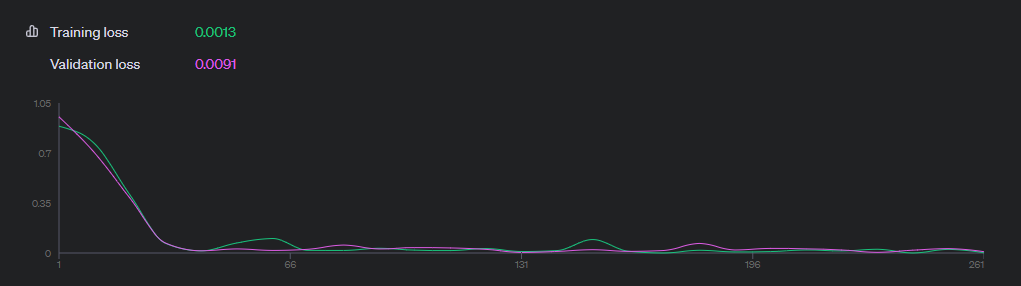
\includegraphics[width=1\textwidth]{LATEX/Appendices/Images/Software/AI Model/training_validation_loss_graph.png}
    \caption{Training Loss Graph}
    \label{fig:training_loss_graph}
\end{figure}

The training process demonstrated a significant reduction in both training and validation loss as the number of steps increased, suggesting effective learning and generalisation capabilities of the model. The detailed loss metrics, captured over 261 steps, show an initial high loss that gradually stabilises, reflecting the model’s adaptation to the complexities of translating legal contracts into Solidity code.

\begin{figure}[!ht]
    \centering
    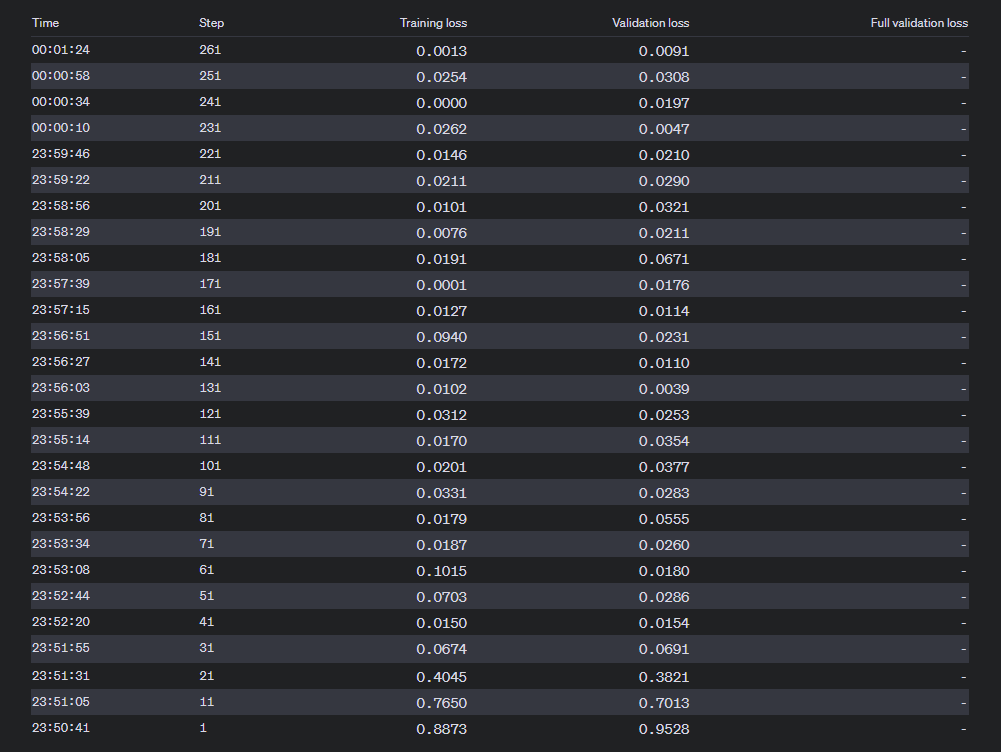
\includegraphics[width=1\textwidth]{LATEX/Appendices/Images/Software/AI Model/training_validation_loss_table.png}
    \caption{Training Loss Table}
    \label{fig:training_loss_table}
\end{figure}

\section{Backend}

Since the training of the AI model for contract conversions has concluded, the next step is to proceed with the backend implementation. As mentioned in the previous chapter, this will be done using \texttt{Django REST API}. 

\subsection{Project Structure}

The backend of our mobile application, referred to as \texttt{ASACBackEnd}, consists of several Django apps that handle different functionalities of the application. In addition, the root directory contains a few files meant for  configuration and utility purposes:

\begin{itemize}
    \item \textbf{requirements.txt:} This file lists all the Python packages that the project depends on. It is used to install all necessary libraries when setting up the project in a new environment.
    \item \textbf{manage.py:} This is a command-line utility that allows interaction with the Django project. It acts as a thin wrapper around the \textit{django-admin} command-line tool for carrying out administrative tasks.
    \item \textbf{.coveragerc:} This file describes settings for code coverage reports, which help in tracking the amount of code tested as part of the quality control. 
    \item \textbf{pytest.ini:} This file configures various aspects of pytest, a framework for testing Python code. It includes settings that influence the discovery of test modules and their behaviour.
\end{itemize}

Apart from that, the root directory includes the \texttt{``staticfiles''} folder, which contains the following:

\begin{itemize}
    \item \textbf{admin folder:} Houses custom style-sheets, scripts, and images specifically for the Django admin interface, making it aesthetically pleasing.
    \item \textbf{rest\_framework folder:} Accommodates static files for the Django REST Framework's browsable API. These files improve the interface's aesthetics.
\end{itemize}

Additionally, every \textit{Django app} of the project includes a directory called \texttt{``tests''} containing test files corresponding to each module written.

\subsection{Root Application}

The root application, \texttt{``ASACBackEnd''}, serves as the core of our backend architecture and includes several key configuration files that define the operational settings and the application's entry points. The naming similarity with the Django project's root follows from the adherence to Django naming conventions.

\subsubsection{Django Application Settings}

The \texttt{settings.py} includes the following key configurations:
\begin{itemize}
    \item \textbf{SECRET\_KEY:} A key used for cryptographic signing, crucial for maintaining security in production.
    \item \textbf{DEBUG:} A flag that turns on/off debug mode. It is enabled here for development purposes but will be disabled in a production environment later during deployment.
    \item \textbf{DATABASES:} The development configuration uses SQLite, while the production uses PostgreSQL.
    \item \textbf{STATIC and MEDIA SETTINGS:} Define how static files and uploaded media are handled by the application. These are primarily used for the admin site. 
    \item \textbf{CORS SETTINGS:} Configured to allow cross-origin requests from predefined origins, essential for API interactions in a distributed environment.
\end{itemize}

\subsubsection{Web Server Gateway Interface (\textit{WSGI}) Configuration}

The \textit{Django} application is configured for \textit{WSGI} in the \texttt{wsgi.py} file. With the following in place, a web server is enabled to communicate and consequently handle web requests and responses.

\subsubsection{Asynchronous Server Gateway Interface (asgi) and Channels Configuration}

An instance of the \textit{ASGI} application is set up to receive \texttt{asynchronous} \textit{HTTP} and \textit{WebSocket} protocols in the \texttt{asgi.py} file. This is important for real-time features like notifications and live updates for the forums.

\subsubsection{URL Routing}

\texttt{urls.py} file manages URL patterns across the entire application, directing requests to appropriate views.

\subsection{Accounts Application}

The \texttt{``Accounts''} module within \texttt{ASACBackEnd} handles all functionalities related to user management, including registration, authentication, and the management of authentication tokens.

\subsubsection{Admin} 

The \textit{admin.py} file facilitates administrative management by establishing a connection between the Django admin interface and the user \& token models.

\subsubsection{Apps} 

This \textit{apps.py} file defines the \texttt{Accounts} application configuration, setting up essential application properties and metadata.

\subsubsection{Models} 

The \textit{models.py} file contains the \textit{User} and \textit{AuthenticationPushToken} models. The User model extends \textit{Django's} \textit{AbstractUser}, adding extra fields and validations for them. The \textit{AuthenticationPushToken} model links users to their unique push tokens.

\subsubsection{Serialisers}

The serialisers in this file handle incoming and outgoing data formats for user-related operations:

\begin{itemize}
    \item \textbf{SignUpSerialiser:} Manages user registration, ensuring data validation, password confirmation, and user creation.
    \item \textbf{UserSerialiser:} Simplifies user data serialisation for common user information retrieval.
    \item \textbf{AuthenticationPushTokenSerialiser:} Manages the creation and upkeep of user tokens for authentication..
\end{itemize}

\subsubsection{URL Configuration}

The URL configuration for the \texttt{Accounts} application defines the endpoints:

\begin{itemize}
    \item \texttt{push-token/} is linked to \texttt{AuthenticationPushTokenView}, which manages the creation and updates of authentication tokens.
    \item \texttt{validate-token/} connects to \texttt{ValidateAuthenticationTokenView}, providing a mechanism to validate user tokens.
    \item \texttt{sign-up/} is handled by \texttt{SignUpView}, facilitating new user registration.
    \item \texttt{login/} routes to \texttt{LoginView}, which supports user login functionality.
\end{itemize}

\subsubsection{Views}

The \textit{Accounts} application's views manage user interactions within the system:

\begin{itemize}
    \item \textbf{ValidateAuthenticationTokenView:} This view verifies the validity of a user's authentication token. It uses \textit{TokenAuthentication} permission to ensure that each request is made by an authenticated user. If authenticated, it returns a confirmation of token validity. Otherwise, it handles exceptions, particularly \textit{AuthenticationFailed}, by returning an invalid token response, indicating the need for re-authentication.
    \item \textbf{LoginView:} Open to all users (\textit{AllowAny} permission), this view manages user login. Upon receiving a username and password, it attempts to authenticate the user. In the case of success, it retrieves or creates a new authentication token for the session and optionally sends a push notification via the associated token. Incorrect credentials will return an error response, maintaining security by denying access.
    \item \textbf{SignUpView:} Also open to all users, this view manages user registration using the \textit{SignUpSerialiser}. It validates the incoming data, creates a new user record, and sets up initial authentication details. The view ensures that all data conforms to predefined security and integrity standards before creating the user record.
    \item \textbf{AuthenticationPushTokenView:} Restricted to authenticated users (\textit{IsAuthenticated} permission), this view manages the lifecycle of authentication tokens. Through \textit{POST}, \textit{GET}, and \textit{DELETE} requests, respectively, users can generate, obtain, and delete tokens. Before proceeding with any operations, the view verifies user's identity. To help with troubleshooting, it provides detailed error messages.
\end{itemize}

\subsection{Contracts Application}

The entire contract handling process, including the creation, validation, and deletion of employment and smart contracts, is handled by the \texttt{``Contracts''} module of \texttt{ASACBackEnd}. Users can generate their contracts directly through our AI model, which we have fine-tuned earlier.

\subsubsection{Admin} 

To enable administrative management, the \textit{admin.py} file registers the \textit{SmartContract} model with Django's admin panel.

\subsubsection{Apps} 

This file sets up the application configuration with Django, defining it within the project's settings.

\subsubsection{Models} 

The \textit{models.py} file defines models like \textit{EmploymentContract} and \textit{SmartContract}, which include fields for managing contract details such as names, blockchain addresses, and content (the legal text of the employment contract and \textit{Solidity} code respectively), along with custom validators.

\subsubsection{Serialisers}

This file has two serialisers: \textit{EmploymentContractSerialiser} and \textit{SmartContractSerialiser}. These handle the conversion between model instances and data types suitable for rendering into JSON or validating data from POST requests, helping in creation and management of contract data.

\subsubsection{URL Configuration}

The URL configuration for the \textit{Contracts} application is designed to manage interactions related to contract operations:

\begin{itemize}
    \item \textbf{generate-contract/} links to \texttt{GenerateContractView}, which is responsible for initiating the generation of new smart contracts.
    \item \textbf{delete-contract/<str:contract\_name>/} connects to \texttt{DeleteContractView}, allowing users to delete specific contracts by name.
    \item \textbf{get-user-contracts/} routes to \texttt{FetchContractsView}, providing a list of all contracts associated with a user.
    \item \textbf{get-valid-checksum-address/} is managed by \texttt{CheckSumAddressView}, which validates Ethereum addresses.
\end{itemize}

\subsubsection{Validators}

Custom validators in \texttt{validators.py} improve data integrity:
\begin{itemize}
    \item \textbf{validate\_ethereum\_address:} Makes sure Ethereum addresses are correctly checksummed to prevent errors in blockchain transactions.
    \item \textbf{validate\_hexadecimal:} Confirms whether entries are valid hexadecimal values.
    \item \textbf{validate\_contract\_name:} Ensures the contract name is within the allowed character limits and uses only permitted characters.
    \item \textbf{validate\_json\_format:} Checks that the JSON format for contract content is correct. This is used for token interfaces that are passed to the smart contract.
\end{itemize}

\subsubsection{Views}

Functionalities of views defined in \texttt{views.py} are as follows:
\begin{itemize}
    \item \textbf{GenerateContractView:} Handles the \textit{POST} request to generate a new smart contract, transforming legal text into Solidity code. It verifies user input, communicates with our optimised AI model via the \textit{OpenAI API}, and stores the newly created smart contract in the database. Users receive notifications when their contracts are successfully generated.
    \item \textbf{DeleteContractView:} Offers users the ability to remove their contracts. After confirming the user's identity i.e. who owns the contract, it permits the contract to be deleted.
    \item \textbf{FetchContractsView:}  Allows users to retrieve a list of their contracts. It filters contracts by the authenticated user and serialises them for the response.
    \item \textbf{CheckSumAddressView:} Verifies user-provided Ethereum addresses to make sure they are accurate and suitable for blockchain transactions.
\end{itemize}

\subsection{Forums Application}

The \texttt{``Forums''} module within \texttt{ASACBackEnd} manages community interactions such as posts, comments, and likes. This application allows users to engage with each other, fostering a community environment within the app.

\subsubsection{Admin}

This file is responsible for configuring the Django admin panel to manage \textit{Post}, \textit{Comment}, and \textit{Like} models.

\subsubsection{Apps}

This file defines the \textit{Forums} app configuration, registering it within the Django project's ecosystem.

\subsubsection{Models} 

This file includes models for \textit{Post}, \textit{Comment}, and \textit{Like}. Each model is tied to the \textit{User} model from the \textit{Accounts} module, making sure all activities are user-specific.

\subsubsection{Serialisers}

The \texttt{Forums} application uses the following serialisers to handle data conversion between model instances and JSON:
\begin{itemize}
    \item \textbf{PostSerialiser:} Serialises post data, including related comments and like count. It includes methods to check if a post has been liked by the user and if the user is the author of the post.
    \item \textbf{CommentSerialiser:} Handles serialisation of comments, showing the username of the comment author.
    \item \textbf{LikeSerialiser:} Serialises like information, specifically tracking which user liked which post.
\end{itemize}

\subsubsection{URL Configuration}

The URL configuration for the \texttt{Forums} application routes user interactions concerning posts, comments, and likes:

\begin{itemize}
    \item \texttt{posts/} is routed to \texttt{PostListCreateView}, which facilitates the listing of all posts and the creation of new ones. This view makes sure users can both retrieve a list of posts and contribute new content within a single interface.
    \item \texttt{posts/<int:pk>/} connects to \texttt{PostDetailView}, which provides detailed information about a specific post. It allows users to retrieve, update, or delete a post based on its unique identifier.
    \item \texttt{posts/<int:pk>/comments/} links to \texttt{CommentCreateView}, enabling users to add comments to posts.
    \item \texttt{posts/<int:pk>/comments/list/} routes to \texttt{CommentListView}, which lists all comments associated with a specific post.
    \item \texttt{posts/<int:pk>/like/} is managed by \texttt{LikeCreateDeleteView}, allowing users to like or unlike a post.
\end{itemize}

\subsubsection{Views}

The views within the \texttt{Forums} module are designed to use \texttt{IsAuthenticatedOrReadOnly} permissions, ensuring that any modification to the data can only be done by authenticated users.

\begin{itemize}
    \item \textbf{PostListCreateView:}
    \begin{itemize}
        \item \textbf{GET:} Fetches and serialises a list of all posts. This operation is available to any user, authenticated or not, ensuring that the forum's content is accessible to the wider public.
        \item \textbf{POST:} Handles the creation of new posts. The view accepts data from authenticated users only, assigning the post authorship automatically to the logged-in user. 
    \end{itemize}

    \item \textbf{PostDetailView:}
    \begin{itemize}
        \item \textbf{GET:} Retrieves and serialises a single post identified by its primary key. Similarly to the \textit{``list''} view, this \textit{``detail''} view is accessible to both authenticated and unauthenticated users.
        \item \textbf{PUT:} Updates a specific post. This operation is strictly guarded to ensure that only the author of the post can make edits, thus preventing unauthorised users from altering content they do not own.
        \item \textbf{DELETE:} Removes the post from the database. Similar to the update operation, deletion is restricted to the post's author.
    \end{itemize}

    \item \textbf{CommentCreateView:}
    \begin{itemize}
        \item This view contributes to the addition of comments to posts. It ensures that each comment is linked to both the user making it and the post under which it is made. User authentication is mandatory, reinforcing that comments can only be created by logged-in users, thereby associating each comment with a specific user identity.
    \end{itemize}

    \item \textbf{CommentListView:}
    \begin{itemize}
        \item Provides a serialisation of all comments associated with a particular post. The comments are presented in reverse chronological order, ensuring that the newest comments are easily accessible. This view is read-only and does not require user authentication, allowing open access to comment data.
    \end{itemize}

    \item \textbf{LikeCreateDeleteView:}
    \begin{itemize}
        \item \textbf{POST:} Manages the creation or deletion of a like for a specific post based on its existence. If a like by the user does not exist, it is created; if it does, it is removed.
        \item \textbf{DELETE:} Explicitly removes a like from a post. This function is safeguarded to only allow the user who created the like to remove it.
        \item \textbf{Notification System:} When a post is liked for the first time, a notification is sent to the post's author, alerting them of the new like.
    \end{itemize}
\end{itemize}

\subsection{Notifications Application}

The \texttt{``Notifications''} module within \texttt{ASACBackEnd} manages everything related to notifications. This includes the registration and deletion of push tokens and the real-time delivery of notifications.

\subsubsection{Admin} 

This file registers the \textit{NotificationPushToken} model with the Django admin for administrative management.

\subsubsection{Apps} 

This file defines the application configuration for the \textit{Notifications} module. It specifies the name of the application and its default auto field.

\subsubsection{Consumers}

\textit{NotificationConsumer} is included in the \textit{consumers.py} file. It manages \textit{WebSocket} connections using \textit{Django Channels} for real-time asynchronous communication between the client and the server. Implementation in the \textit{NotificationConsumer} includes the following functions:

\begin{itemize}
    \item \textbf{connect:}
    \begin{itemize}
        \item Purpose: Establishes the \textit{WebSocket} connection between the client and the server.
        \item Process: When a client attempts to connect, this method is invoked. The consumer adds the connection to a group named \textit{``notification\_group''}. Groups in \textit{Django Channels} are a way to organise multiple connections, allowing messages to be sent to all of them simultaneously.
        \item \textbf{self.channel\_layer.group\_add}: The connect function calls this method to add the current channel to the specified group for broadcasting messages to all clients within it.
        \item \textbf{self.accept}: The connect function calls this method to finalise the \textit{WebSocket} connection, allowing data to be exchanged between the client and the server.
    \end{itemize}

    \item \textbf{disconnect:}
    \begin{itemize}
        \item Purpose: Handles the disconnection of a client from the server.
        \item Process: When a client disconnects, whether due to closing the mobile application or losing connection, this method removes the channel from the group, cleaning up resources and preventing further communication to a non-existent connection.
        \item \textbf{self.channel\_layer.group\_discard}: The disconnect function calls this method passing it the group and channel to remove the latter from the former.
    \end{itemize}

    \item \textbf{receive:}
    \begin{itemize}
        \item Purpose: Receives messages from \textit{WebSocket} clients.
        \item Process: When a message is received, this method processes it, confirms receipt by sending a message back to the client, and broadcasts it to all clients in the group.
        \item \textbf{self.send}: Sends a confirmation message back to the client who originated the request.
        \item \textbf{self.channel\_layer.group\_send}: Broadcasts the received message to all clients in the group.
    \end{itemize}

    \item \textbf{notification\_message:}
    \begin{itemize}
        \item Purpose: Distributes messages received from the \textit{group\_send} action.
        \item Process: This method is called when a message is broadcast to the group. It receives the event, which includes the message data, and then sends it to the client.
        \item \textbf{self.send}: Sends the final text data to the clients.
    \end{itemize}
\end{itemize}

\subsubsection{Models}

The \textit{models.py} file defines the \textit{NotificationPushToken} model. It links a unique notification token with a user and includes fields for the token string, creation timestamp, and a user foreign key.

\subsubsection{Routing}

Web socket URL patterns are defined in \textit{routing.py} to route notification-related \textit{WebSocket} connections to the appropriate consumer.

\begin{itemize}
    \item \textit{ws/notifications/} is routed to \textit{NotificationConsumer.as\_asgi()}. The use of the \textit{.as\_asgi} method dictates that the consumer is prepared to handle asynchronous gateway interface applications, suitable for real-time \textit{WebSocket} communications.
\end{itemize}

\subsubsection{Serialisers}

The serialisers in \textit{serialisers.py} allow the conversion of model instances into JSON format for API responses and vice versa, specifically \textit{NotificationPushTokenSerialiser} was implemented to manage serialisation and deserialisation of the \textit{NotificationPushToken} data. It handles token creation and updates while ensuring that the creation date is read-only.

\subsubsection{URL Configuration}

The URL configuration within the \textit{Notifications} module is outlined in the \textit{urls.py} file, which specifies the routes for managing notification tokens:

\begin{itemize}
    \item \textbf{save-token/} is connected to \textit{SaveTokenView}.
    \item \textbf{delete-token/} is linked to \textit{DeleteTokenView}.
\end{itemize}

\subsubsection{Utilities}

The \textit{utils.py} file includes a utility function called \textit{send\_push\_notification} that utilises the \textit{exponent\_server\_sdk} to send push notifications to users. It handles message creation and delivery, catching and logging any errors that occur during the process.

\subsubsection{Views}

Views in the \textit{Notifications} module handle API requests related to notification tokens:

\begin{itemize}
    \item \textbf{SaveTokenView:} Allows authenticated users to save or update their notification tokens. The view checks the validity of the data using the corresponding serialiser and saves the token if valid.
    \item \textbf{DeleteTokenView:} Permits authenticated users to delete their notification tokens.
\end{itemize}

\subsection{Database Configuration}

The database is configured as follows:

\begin{itemize}
    \item \textbf{Database Engine:} As previously outlined, \textit{PostgreSQL} was selected as the main database system for the \textit{ASACBackEnd} project because of its capabilities for complex queries and data integrity.
    \item \textbf{Database Name:} The database for the production environment is named \textit{``asacbackenddb''}.
    \item \textbf{Credentials:} Access to the database is secured with a username and password.
    \item \textbf{Host and Port:} The database is hosted locally on the deployment server with the default PostgreSQL port. With this configuration, database operations have quick access and reduced latency within the internal network.
    \item \textbf{Connection Settings:} By limiting access to trusted, secure sources, the database is configured to accept connections from specific IP addresses across the United Kingdom, hence enhancing security. This might be subject to change in the future.
    \item \textbf{Backup and Recovery:} To ensure data durability and dependability, regular backups are scheduled and broad recovery procedures are in place to manage any potential data loss.
\end{itemize}

\section{Frontend}

Having developed the backend, we now shift our focus to the frontend implementation. As outlined in the design chapter, \texttt{ASACFrontEnd} utilises \texttt{React Native} with \texttt{JavaScript} to build the UI. 

\subsection{Project Structure}

In the root directory we have the following configuration files:

\begin{itemize}
    \item \textbf{App.js:} Serves as the root component of our application. It initialises the navigation container and global providers such as authentication, theme, and keyboard handling. Additionally, it configures platform-specific intensifications and notification settings.
    \item \textbf{app.json:} Contains metadata for the application such as the name, version, and configuration specifics for iOS, Android and web. Additionally, it lists the plugins, assets, and other resources that must be included when the app is built.
    \item \textbf{babel.config.js:} Configures the Babel compiler for JavaScript with environment-specific settings for testing and production. This setup specifies how modern JavaScript features are translated into versions that are backward-compatible with older engines.
    \item \textbf{ErrorBoundary.js:} A higher-order component used to catch JavaScript errors anywhere in the child component tree, log those errors, and display a fallback UI instead of the component tree that crashed. This component was extensively used during the development phase for error tracking.
    \item \textbf{package.json:} Defines the project’s dependencies, scripts, and Jest configuration for testing.
    \item \textbf{package-lock.json:} This file is automatically generated when Node packages are installed (using npm) in the project. It serves to lock the versions of each package and its dependencies which were installed, ensuring that every npm install results in the exact same set of dependencies.
\end{itemize}

The components of the project are organised into a main directory called \texttt{``app''}. Inside of it, there are several sub-directories, each handling a different part of the application's functionality:

\begin{itemize}
    \item \textbf{Components Directory:} Houses reusable components for handling authentication, managing notifications, applying consistent theming, and controlling keyboard interactions.
    \item \textbf{Navigation Directory:} Contains navigators that manage screen transitions.
    \item \textbf{Screens Directory:} Houses the individual screens of the \textit{app} alongside the \textit{functional hooks} that control them. Each screen is responsible for rendering the UI components relevant to the specific part of the application it represents.
    \item \textbf{Styles Directory:} Contains styling files that define the visual aspects of the application.
\end{itemize}

The test-related files of the project are consolidated into a primary directory named \texttt{\_\_tests\_\_}.

The project also includes a folder named \texttt{assets} in the root directory, which contains all the static files used in the application.

\subsection{Components Directory}

The \texttt{components} directory is organised to group essential utility components. It includes the following files:

\begin{enumerate}
    \item \texttt{Authentication.js}
    \item \texttt{Keyboard.js}
    \item \texttt{Notifications.js}
    \item \texttt{Theme.js}
\end{enumerate}

\subsubsection{Authentication Component}

\begin{itemize}
    \item \textbf{Context Setup:} The \texttt{AuthContext} is created to store authentication state and functions to manage it. Any component within the application can access it.
    \item \textbf{Token Validation:} \textit{validateToken} function checks the validity of the stored authentication token by making a \textit{GET} request to the backend. This is in place to make sure the user remains logged in even if the application restarts.
    \item \textbf{User Registration and Login:} Functions \textit{signUp} and \textit{login} interact with the backend to register new users or authenticate existing ones and manage the authentication token received from the backend.
    \item \textbf{Logout Functionality:} The \textit{logout} function erases the authentication token from storage, effectively logging out the user.
    \item \textbf{Animation and Alerts:} \textit{LayoutAnimation} is used to provide smooth login and logout transitions, while \textit{Alert} is used to give feedback on authentication procedures.
    \item \textbf{Error Handling:} Includes robust error handling to manage issues during authentication processes, easing troubleshooting and preventing the entire UI from crashing.
    \item \textbf{Higher-Order Component Usage:} Wraps the child components with \textit{WebSocketProvider} if the user is logged in, enabling \textit{WebSocket} connections for notifications.
\end{itemize}

\subsubsection{Keyboard Component}

The \texttt{Keyboard} component is a custom utility developed to manage keyboard interactions and visibility, created in response to issues encountered with \textit{React Native's} built-in \textit{KeyboardAvoidingView}, which at times did not provide reliable behaviour. The problem was that, for some reason, as soon as the \textit{KeyboardAvoidingView} was combined with the \textit{ScrollView}, the screens applying it did not focus on any input fields. To ensure a more consistent user experience, the \textit{Keyboard} component implements custom logic to handle keyboard events and adjust \textit{UI} elements accordingly. 

\begin{itemize}
    \item \textbf{Context Setup:} The \textit{KeyboardProvider} component utilises the \textit{React context API}, wrapping the application's component tree to make keyboard states and functionalities accessible across the entire application. This is achieved through the \textit{useKeyboard} hook.
    \item \textbf{State Management:} It maintains \textit{keyboardHeight} and \textit{isKeyboardVisible} states to provide real-time keyboard status.
    \item \textbf{Event Listeners:} The component sets up event listeners for keyboard \textit{show} and \textit{hide} actions. In order to keep the keyboard from covering input fields, it computes the keyboard height and modifies the layout when it is displayed. Conversely, when the keyboard hides, it resets adjustments to the layout.
    \item \textbf{Scroll Handling:} Its capacity to control scrolling actions in response to keyboard visibility is one of its primary characteristics. The component makes sure that when an input field is focused, it scrolls into view, avoiding being obscured by the keyboard. This is handled by using the \textit{registerScrollViewRef} and \textit{scrollResponderScrollNativeHandleToKeyboard} methods, respectively.
    \item \textbf{Layout Animation:} \textit{LayoutAnimation} is used for smooth transitions and layout changes when the keyboard shows or hides.
    \item \textbf{Clean-Up Logic:} To prevent memory leaks, the component cleans up event listeners when it unmounts or the provider is removed from the component tree.
\end{itemize}

\subsubsection{Notifications Component}

The \texttt{useWebSocket} hook manages a \textit{WebSocket} connection for real-time asynchronous notification functionality. Here is how it is set up:

\begin{itemize}
    \item Connection is initiated with \textit{WebSocket(url)}, which switches between \textit{wss://} and \textit{ws://} based on the backend's \textit{URL} schema for secure connections.
    \item \textbf{Event Listeners:}
        \begin{itemize}
            \item \textit{onopen:} Confirms the connection has been successfully opened and logs it to the console.
            \item \textit{onmessage:} Listens for incoming messages, then parses them, and finally triggers a notification using \textit{Expo's notification API}. This is in place to make sure that users receive alerts even when the application is not actively in use.
            \item \textit{onerror:} Handles any errors that occur during the web socket communication.
            \item \textit{onclose:} Records reasons for web socket disconnections.
        \end{itemize}
    \item Lastly, when the component unmounts, the hook makes certain the web socket connection is correctly terminated.
\end{itemize}

The component also handles push notifications through a series of functions designed to manage user tokens and permissions:

\begin{itemize}
    \item \textbf{savePushToken:} Gets a push token from \textit{Expo's notification service} and sends it to the backend server, where it is stored and associated with the user's account. This token allows the server to send push notifications to the right device.
    \item \textbf{deletePushToken:} Removes a user's token from the backend, stopping push notifications to that device.
    \item \textbf{requestNotificationPermission:} Before any notifications can be sent, the application must request and obtain permission from the user. This function handles this flow and checks the current permission status.
\end{itemize}

To make the web socket functionality accessible throughout the application, the \texttt{WebSocketProvider} component wraps the children in a context provider.

\subsubsection{Theme Component}

\begin{itemize}
    \item \textbf{Context Setup:} Spreads the theme state across the component hierarchy by utilising \textit{React's Context API}.
    \item \textbf{Persistent Theme Option:} The user's theme preference is stored persistently using \textit{expo-secure-store}, maintaining the preferred option across sessions.
    \item \textbf{Theme Switching:} Provides a \textit{toggleTheme} function, which allows users to switch between ``light'' and ``dark'' modes, updating the state within the context accordingly.
    \item \textbf{Dark Mode Support:} The \textit{isDarkMode} flag enables a check that components can use to determine if the dark mode is currently enabled, allowing for conditional styling.
\end{itemize}

The \texttt{ThemeProvider} attempts to retrieve the stored theme from safe storage when it first initialises. If a theme is saved, it sets this as the current one; otherwise, it defaults to \textit{``light''}. This setup is handled within a \textit{useEffect} hook to ensure it runs once when the component mounts.

\subsection{Navigation Directory}

The \texttt{navigation} directory is structured to facilitate user movement and access across different parts of the application. It includes the following files:

\begin{enumerate}
    \item \texttt{AppNavigator.js}
    \item \texttt{PreLoginStack.js}
    \item \texttt{PostLoginTabs.js}
\end{enumerate}

\subsubsection{AppNavigator Component}

The \texttt{AppNavigator} component acts as the primary navigation controller, directing the flow based on the user's authentication status.

\begin{itemize}
    \item To determine if the user is logged in, the component makes use of the \textit{AuthContext}. This context specifies which navigator to render based on a boolean \textit{isLoggedIn} state.
    \begin{itemize}
        \item \textit{AppNavigator} renders the \textit{PostLoginTabs} component if the user is authorised. Otherwise, it defaults to \textit{PreLoginStack}.
    \end{itemize}
    \item The \textit{SafeAreaProvider} wraps the navigator, guaranteeing that the user interface elements are displayed inside the secure regions of a device's display. This is needed to correctly handle the user interface on devices that have disruptions.
\end{itemize}

\subsubsection{PreLoginStack Component}

This stack navigator guides users through the initial authentication process with a structured sequence of screens. The component is comprised of the following features:

\begin{itemize}
    \item \textbf{Stack Navigator:} Utilises the \textit{createStackNavigator} from \textit{@react-navigation/stack} to arrange a series of screens. The stack includes \textit{PreLoginScreen}, which is configured as the initial route, \textit{LoginScreen}, and \textit{SignUpScreen}. This navigator is ideal for managing a sequence of screens where each new screen is placed on top of a stack and where the back action would pop the current screen off the stack to reveal the previous one.    
    \item \textbf{Screen Options:} The \textit{screenOptions} prop is set to \textit{ {\tt {\char '173}} headerShown: false {\tt {\char '175}} }, providing a cleaner user interface that maximises screen space and minimises distraction.
\end{itemize}

\subsubsection{PostLoginTabs Component}

The \texttt{PostLoginTabs} component allows users to switch easily between different sections of the app post-login. 

\begin{itemize}
    \item \textbf{Tab Navigation:} Applies a bottom tab navigator to offer a user-friendly way of switching between the app's main functionalities, such as \textit{home}, \textit{forum}, \textit{support}, and \textit{settings}. Each tab is associated with a specific stack navigator or screen, enabling modular navigation within the app. The navigator starts at the \textit{``Home''} tab, making it the first screen users see upon logging in. 
    \item \textbf{Icon Integration:} Utilises icons from \textit{Ionicons}, which dynamically change based on the focus state, indicating which tab is active.
    \item \textbf{Stack Navigators:} Incorporates multiple stack navigators for the \textit{home} and \textit{forum} tabs to manage more complex navigation paths that include multiple screens. For instance, the home tab can navigate to an editor screen, and the forum tab to a comment screen, both without leaving the tab context.
    \item \textbf{Theme Context:} Uses the \textit{ThemeContext} to adapt the styling of the navigation bar and other UI elements according to the selected theme. 
\end{itemize}

\subsection{Styles Directory}

The \texttt{styles} directory unifies the stylistic guidelines and guarantees a unified appearance across the application. The directory includes the following files:

\begin{enumerate}
    \item \texttt{ThemeStyles.js}
    \item \texttt{GloballySharedStyles.js}
    \item \texttt{LocallySharedStylesPreLoginScreens.js}
    \item \texttt{LocallySharedStylesForumScreens.js}
    \item \texttt{LocallySharedStylesHomeScreens.js}
    \item \texttt{LocallySharedStylesSettingsScreens.js}
    \item \texttt{LocallySharedStylesSupportScreens.js}
\end{enumerate}

\subsubsection{ThemeStyles Component}

The code snippet in this file defines a JavaScript object, \texttt{themeStyles}, which contains two sets of styles corresponding to the light and dark themes.

\begin{itemize}
    \item \textbf{backgroundColour, textColour, inputBackground, borderColour, containerBackground, cardBackground:} These properties control the main colour attributes of the UI components.
    \item \textbf{shadowColour, shadowOpacity:} By defining the shadows for UI elements, these attributes improve the visual contrast and distinction between components. The opacity settings are adjusted to make shadows more pronounced in the dark theme compared to the light one.
\end{itemize}

\subsubsection{GloballySharedStyles Component}

All of the application's screens make considerable use of style definitions, which are stored in the \texttt{GloballySharedStyles} component. The styles are dynamically generated based on the current theme, which is passed as a parameter through the \textit{ThemeStyles} component. The styles are defined using \textit{React Native's} \textit{StyleSheet.create} method. Important Style Categories consist of:

\begin{itemize}
    \item \textbf{Navigation and Layout:} The component defines styles for the tab bar and various containers. The tab bar style, for instance, includes customised active and inactive tint colours, background colour, and positioning to create a floating effect at the bottom of the screen. Container styles are adjusted for general use and, in certain circumstances, for particular contexts like modals and card views. They include settings for alignment, padding, and background colours.
    \item \textbf{Text and Typography:} A range of text styles are provided for different textual content across the UI, such as headers, general text, and modal text. These styles modify the font's weight, colour, and size based on the theme.
    \item \textbf{Interactive Elements:} Styles for buttons, file drop zones and input fields are included, defining dimensions, colour schemes, border characteristics, and alignment. To preserve functional clarity, extra care is taken with components such as exit buttons and activity indicators.
    \item \textbf{Visual Enhancements:} Extra styles such as shadows, separators, and positioning are added to make the UI more attractive.
\end{itemize}

\subsubsection{LocallySharedStyles Components}

The \texttt{LocallySharedStyles} components are utilised to:
\begin{itemize}
    \item Provide custom styling for particular screens within the application that require specific aesthetics not covered by global styles.
    \item Improve maintainability of style code by segregating local styles into dedicated modules. This reduces clutter in main component files.
    \item Allow each screen to independently control its visual elements without impacting other parts of the application, thereby easing more focused style adjustments.
\end{itemize}

The naming structure for the \textit{LocallySharedStyles} components follows a consistent pattern, prefixed with \textit{LocallySharedStyles} followed by the name of the specific component or screen they style, such as \textit{LocallySharedStylesHomeScreen.js} or \textit{LocallySharedStylesSupportScreen.js}. 

\subsection{Screens Directory}

The \texttt{Screens} directory is divided into two main subdirectories in order to control the user interfaces according to the status of authentication. The \texttt{PreLoginScreens} subdirectory contains:

\begin{itemize}
    \item \texttt{PreLoginScreen.js} - Provides introductory page functionalities.
    \item \texttt{LoginScreen.js} - Manages the user login interface.
    \item \texttt{SignUpScreen.js} - Handles user registration interface.
\end{itemize}

Users interact with screens arranged under the \texttt{PostLoginScreens} subdirectory after successfully logging in. This folder is further divided into four directories, each of which stands for a different functional area of the application:

\begin{enumerate}
    \item \textbf{Home:} Focuses on core functionalities such as contract creation and viewing. Files include:
    \begin{itemize}
        \item \texttt{HomeScreen.js} - The main dashboard screen for contract management.
        \item \texttt{ContractItem.js} - Displays individual contract items that are incorporated into the home screen. However, due to the frequent use of custom animations and states there, it was decided to segregate it into a separate file.
        \item \texttt{EditorScreen.js} - Provides an editor for contract viewing.
        \item \texttt{UseHomeScreen.js} - Custom hook for managing home screen states and logic.
        \item \texttt{UseEditorScreen.js} - Custom hook for editor functionalities.
    \end{itemize}
    \item \textbf{Forum:} Enables community interaction. Files include:
    \begin{itemize}
        \item \texttt{ForumScreen.js} - Main screen for forum discussions, where users can post.
        \item \texttt{CommentScreen.js} - Handles the display and management of comments for posts.
        \item \texttt{UseForumScreen.js} - Custom hook for forum screen logic.
        \item \texttt{UseCommentScreen.js} - Custom hook for comment functionalities.
    \end{itemize}
    \item \textbf{Support:} Offers support and help resources to the users. Files include:
    \begin{itemize}
        \item \texttt{SupportScreen.js} - Screen for user support and assistance.
    \end{itemize}
    \item \textbf{Settings:} Manages user preferences and application settings. Files include:
    \begin{itemize}
        \item \texttt{SettingsScreen.js} - Provides interfaces for adjusting user settings.
        \item \texttt{UseSettingsScreen.js} - Custom hook for settings management.
    \end{itemize}
\end{enumerate}

\paragraph{Additional Information}

All the UI components below will perform the functionalities discussed in this section. They are listed here once; future references may be omitted to avoid redundancy, as these code snippets are integrated into all the files described below.

\begin{itemize}
    \item The current theme is obtained from the \textit{ThemeContext}.
    \item Shared and local styles are generated based on the current theme.
    \item State variables are declared using the \textit{useState} hook.
    \item A reference for the \textit{ScrollView} component is created using \textit{useRef}.
    \item Keyboard height is managed using the \textit{useKeyboard} hook.
    \item The \textit{useFocusEffect} hook is used to register and unregister the \textit{ScrollView} reference when the component gains and loses focus.
    \item Interacting with navigation buttons is facilitated through the \textit{React's Navigation library}. The navigation prop is passed to the component, enabling it to command transitions to other screens within the application.
\end{itemize}

\subsubsection{PreLoginScreens: PreLoginScreen.js}

The \texttt{PreLoginScreen.js} uses the \textit{ImageBackground} component to make the screen more engaging. It is divided into three primary interactive sections, which include:

\begin{enumerate}
    \item \textbf{Login Button:} Directs users to the \textit{LoginScreen}.
    \item \textbf{Sign Up Button:} Leads new users to the \textit{SignUpScreen}.
    \item \textbf{About Us Button:} This button is designed to provide users with more information about the software. 
\end{enumerate}

\begin{figure}[!ht]
    \centering
    \includegraphics[width=0.5\textwidth]
    {LATEX/Appendices/Images/Software/Frontend/pre_login_screen.png}
    \caption{Pre Login Screen Appearance}
    \label{fig:pre login screen}
\end{figure}

\subsubsection{PreLoginScreens: LoginScreen.js}

The rendering of the login screen is handled by the \texttt{LoginScreen} functional component. To control the login procedure, this component retrieves the \textit{handleLogin} method from the \textit{AuthContext}. The component returns a view hierarchy structured as follows:

\begin{itemize}
    \item A \textit{View} component that serves as the main container, with styles adjusted based on the keyboard height.
    \item A \textit{StatusBar} component to manage the appearance of the status bar based on the current theme.
    \item A \textit{ScrollView} component, which is referenced to manage keyboard interactions, that allows for scrolling when the content exceeds the screen height.
    \item Inside of it, there is a nested \textit{View} component that contains:
    \begin{itemize}
        \item Another \textit{View} component with a \textit{card} style, housing the \textit{TextInput} fields for username and password inputs.
        \item A \textit{TouchableOpacity} component that acts as the login button, triggering the \textit{handleLogin} function with the entered username and password when pressed.
    \end{itemize}
    \item A separator line at the bottom, with its position adjusted based on the keyboard height.
\end{itemize}

\begin{figure}[!ht]
    \centering
    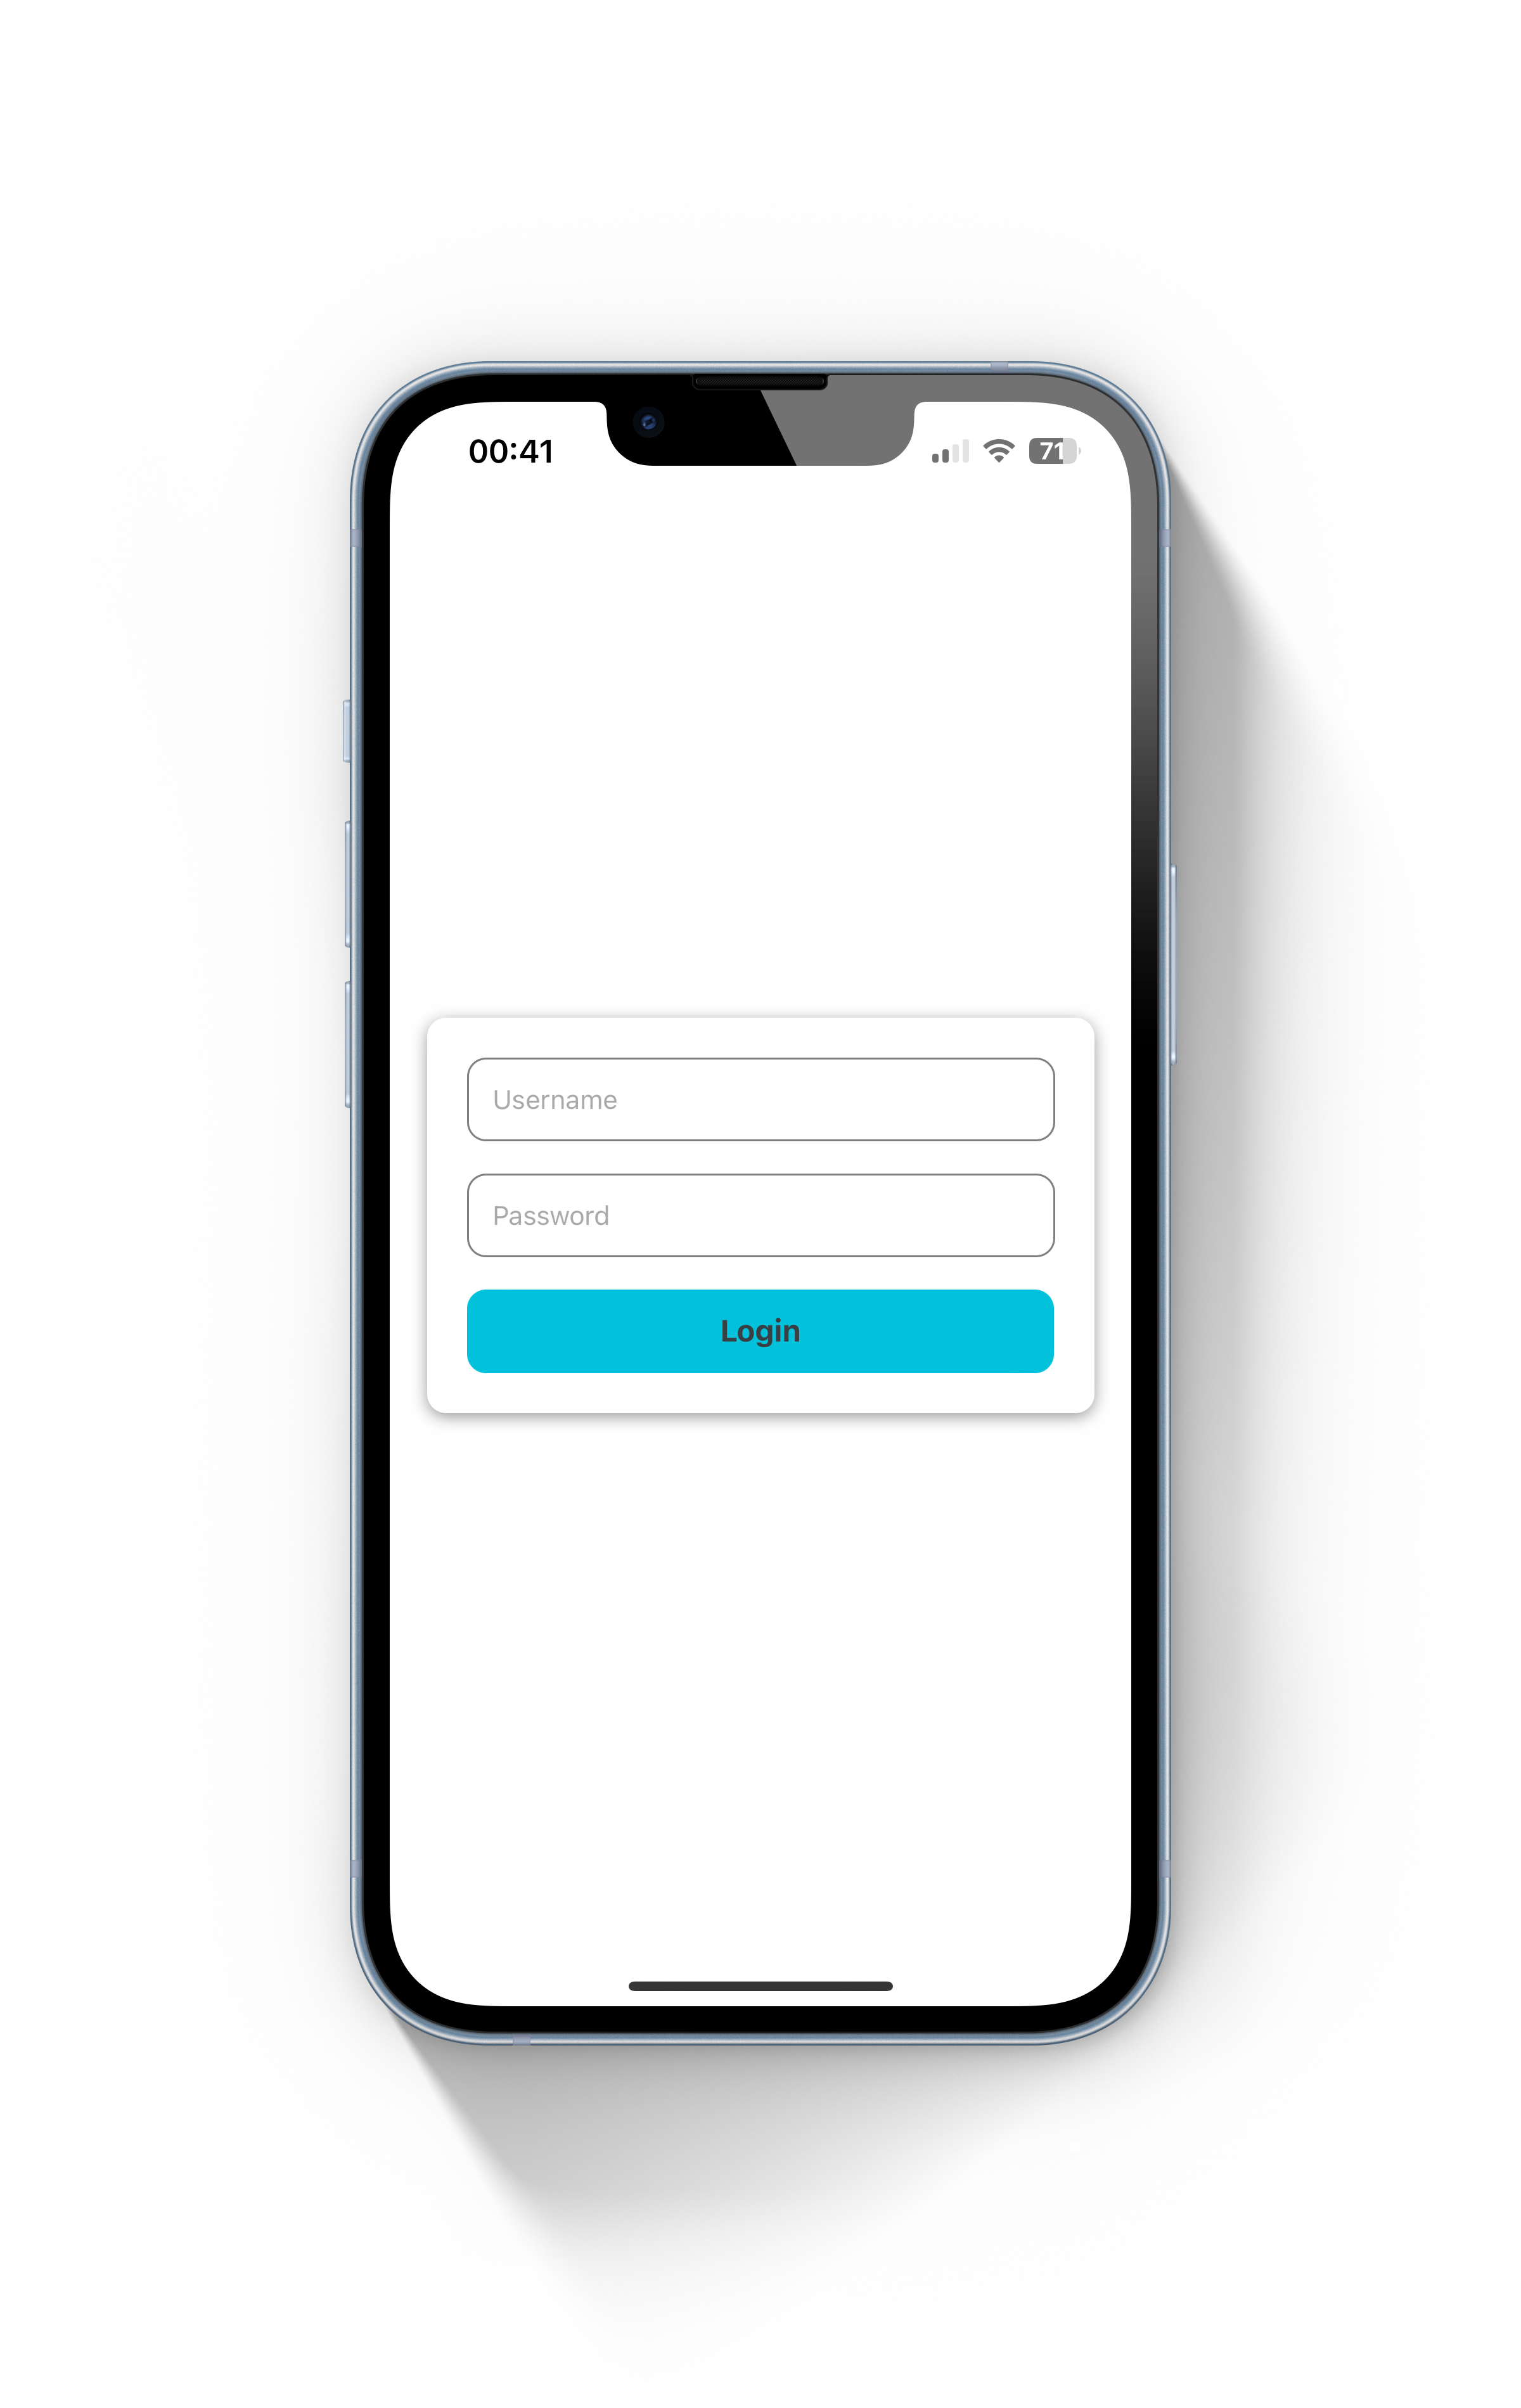
\includegraphics[width=0.5\textwidth]
    {LATEX/Appendices/Images/Software/Frontend/login_screen.png}
    \caption{Login Screen Appearance}
    \label{fig:login screen}
\end{figure}

\subsubsection{PreLoginScreens: SignUpScreen.js} 

The rendering of the sign-up screen is managed by the \texttt{SignUpScreen} functional component. Within this component, the \textit{handleSignUp} function is retrieved from the \textit{AuthContext} to manage the sign-up process. The component gives back a view hierarchy with the following structure:

\begin{itemize}
    \item A \textit{View} component that serves as the main container, with styles adjusted based on the keyboard height. 
    \item A \textit{StatusBar} component to manage the appearance of the status bar based on the current theme. It is important to note that this component is repeatedly added at the individual level of the pre-login screens since it could not be added to the root container, \textit{PreLoginStack}. The \textit{PreLoginScreen} is an exception, as the background image there is too dark, making its components invisible in case of a dark mode. Hence, this component is manually added to each individual screen, contrary to the \textit{PostLoginTabs}, where it was added once at the root component.
    \item A \textit{ScrollView} component, which is referenced to manage keyboard interactions, that allows for scrolling when the content exceeds the screen height. 
    \item Inside the \textit{ScrollView}, a nested \textit{View} component contains:
    \begin{itemize}
        \item Another \textit{View} component with a card style, housing the \textit{TextInput} fields for username, first name, last name, email, password, and password confirmation.
        \item A \textit{TouchableOpacity} component that acts as the sign-up button, triggering the \textit{handleSignUp} function with the entered details and current error state when pressed.
        \item An error icon that appears if there are validation errors, which triggers the display of a modal with error details when pressed.
    \end{itemize}
    \item The error modal, which displays a list of validation errors and allows the user to close it through the exit button.
    \item A separator line at the bottom, with its position adjusted based on the keyboard height.
\end{itemize}

\begin{figure}[!ht]
    \centering
    % Begin the first minipage for the first image
    \begin{minipage}{0.49\textwidth}
        \centering
        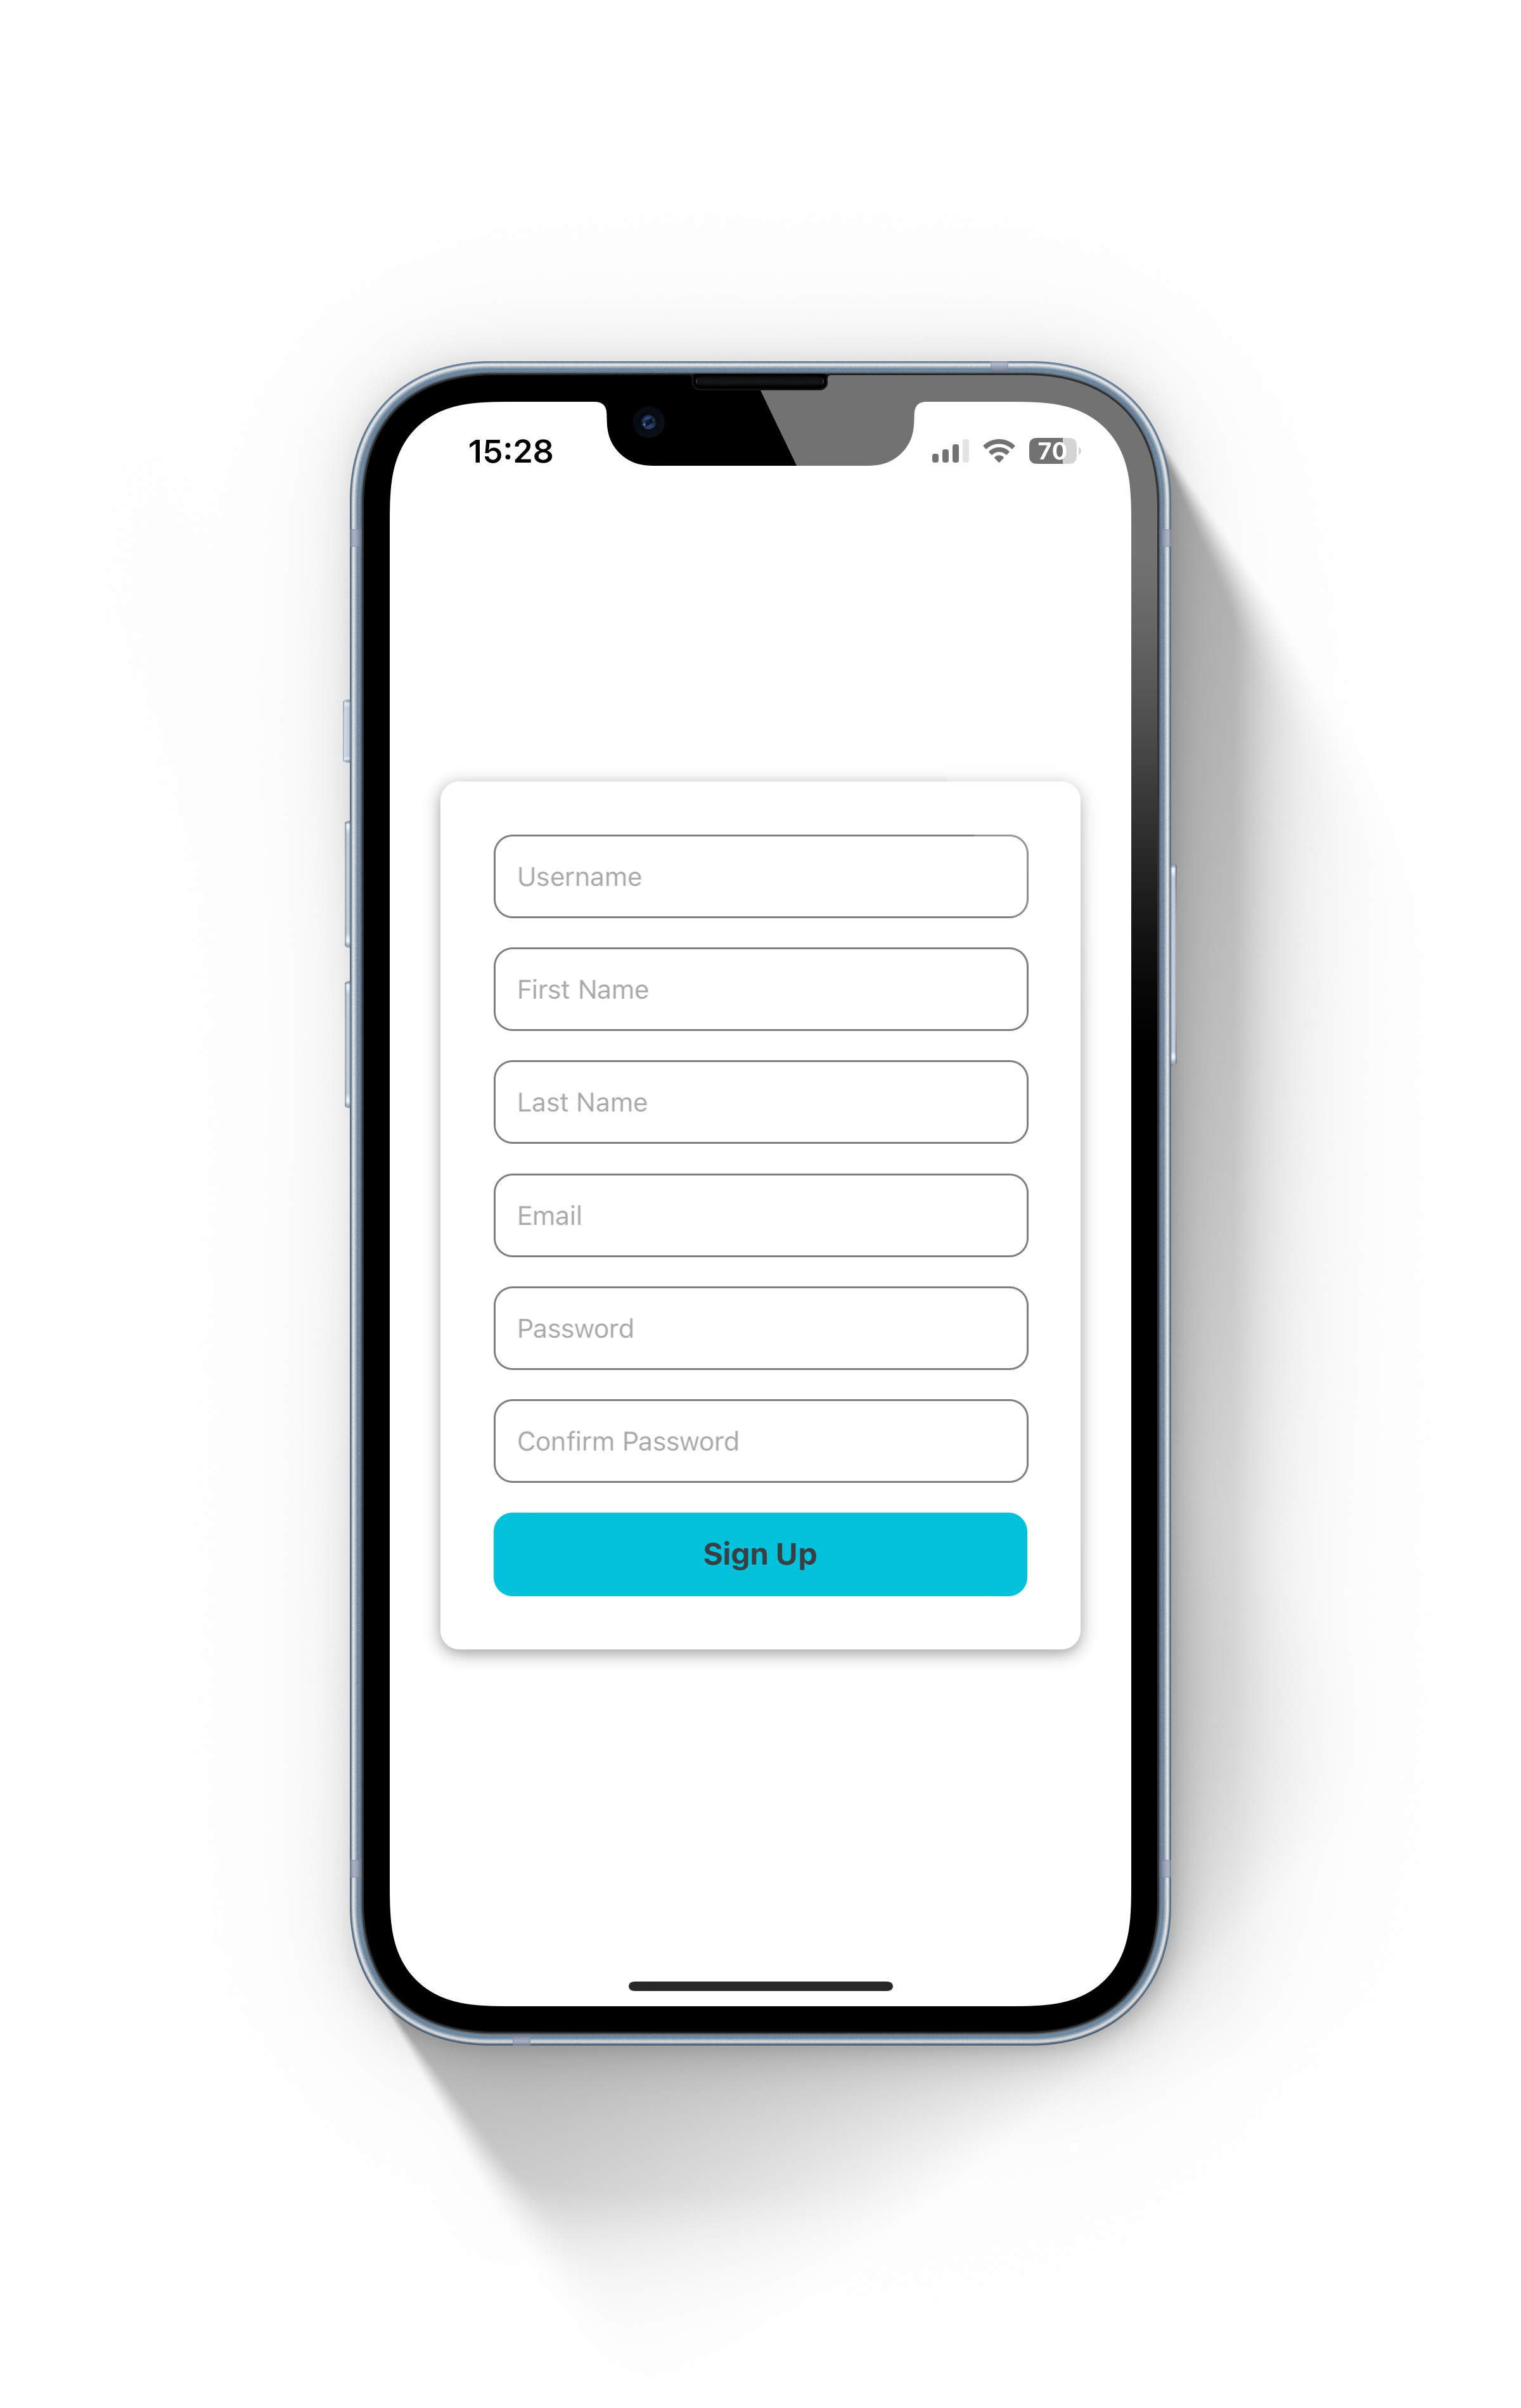
\includegraphics[scale=0.1]{LATEX/Appendices/Images/Software/Frontend/sign_up_screen_1.png}
        \caption{Sign Up Screen 1 Appearance}
        \label{fig:sign up screen 1}
    \end{minipage}\hfill % Insert a small horizontal space between the minipages
    % Begin the second minipage for the second image
    \begin{minipage}{0.49\textwidth}
         \centering
        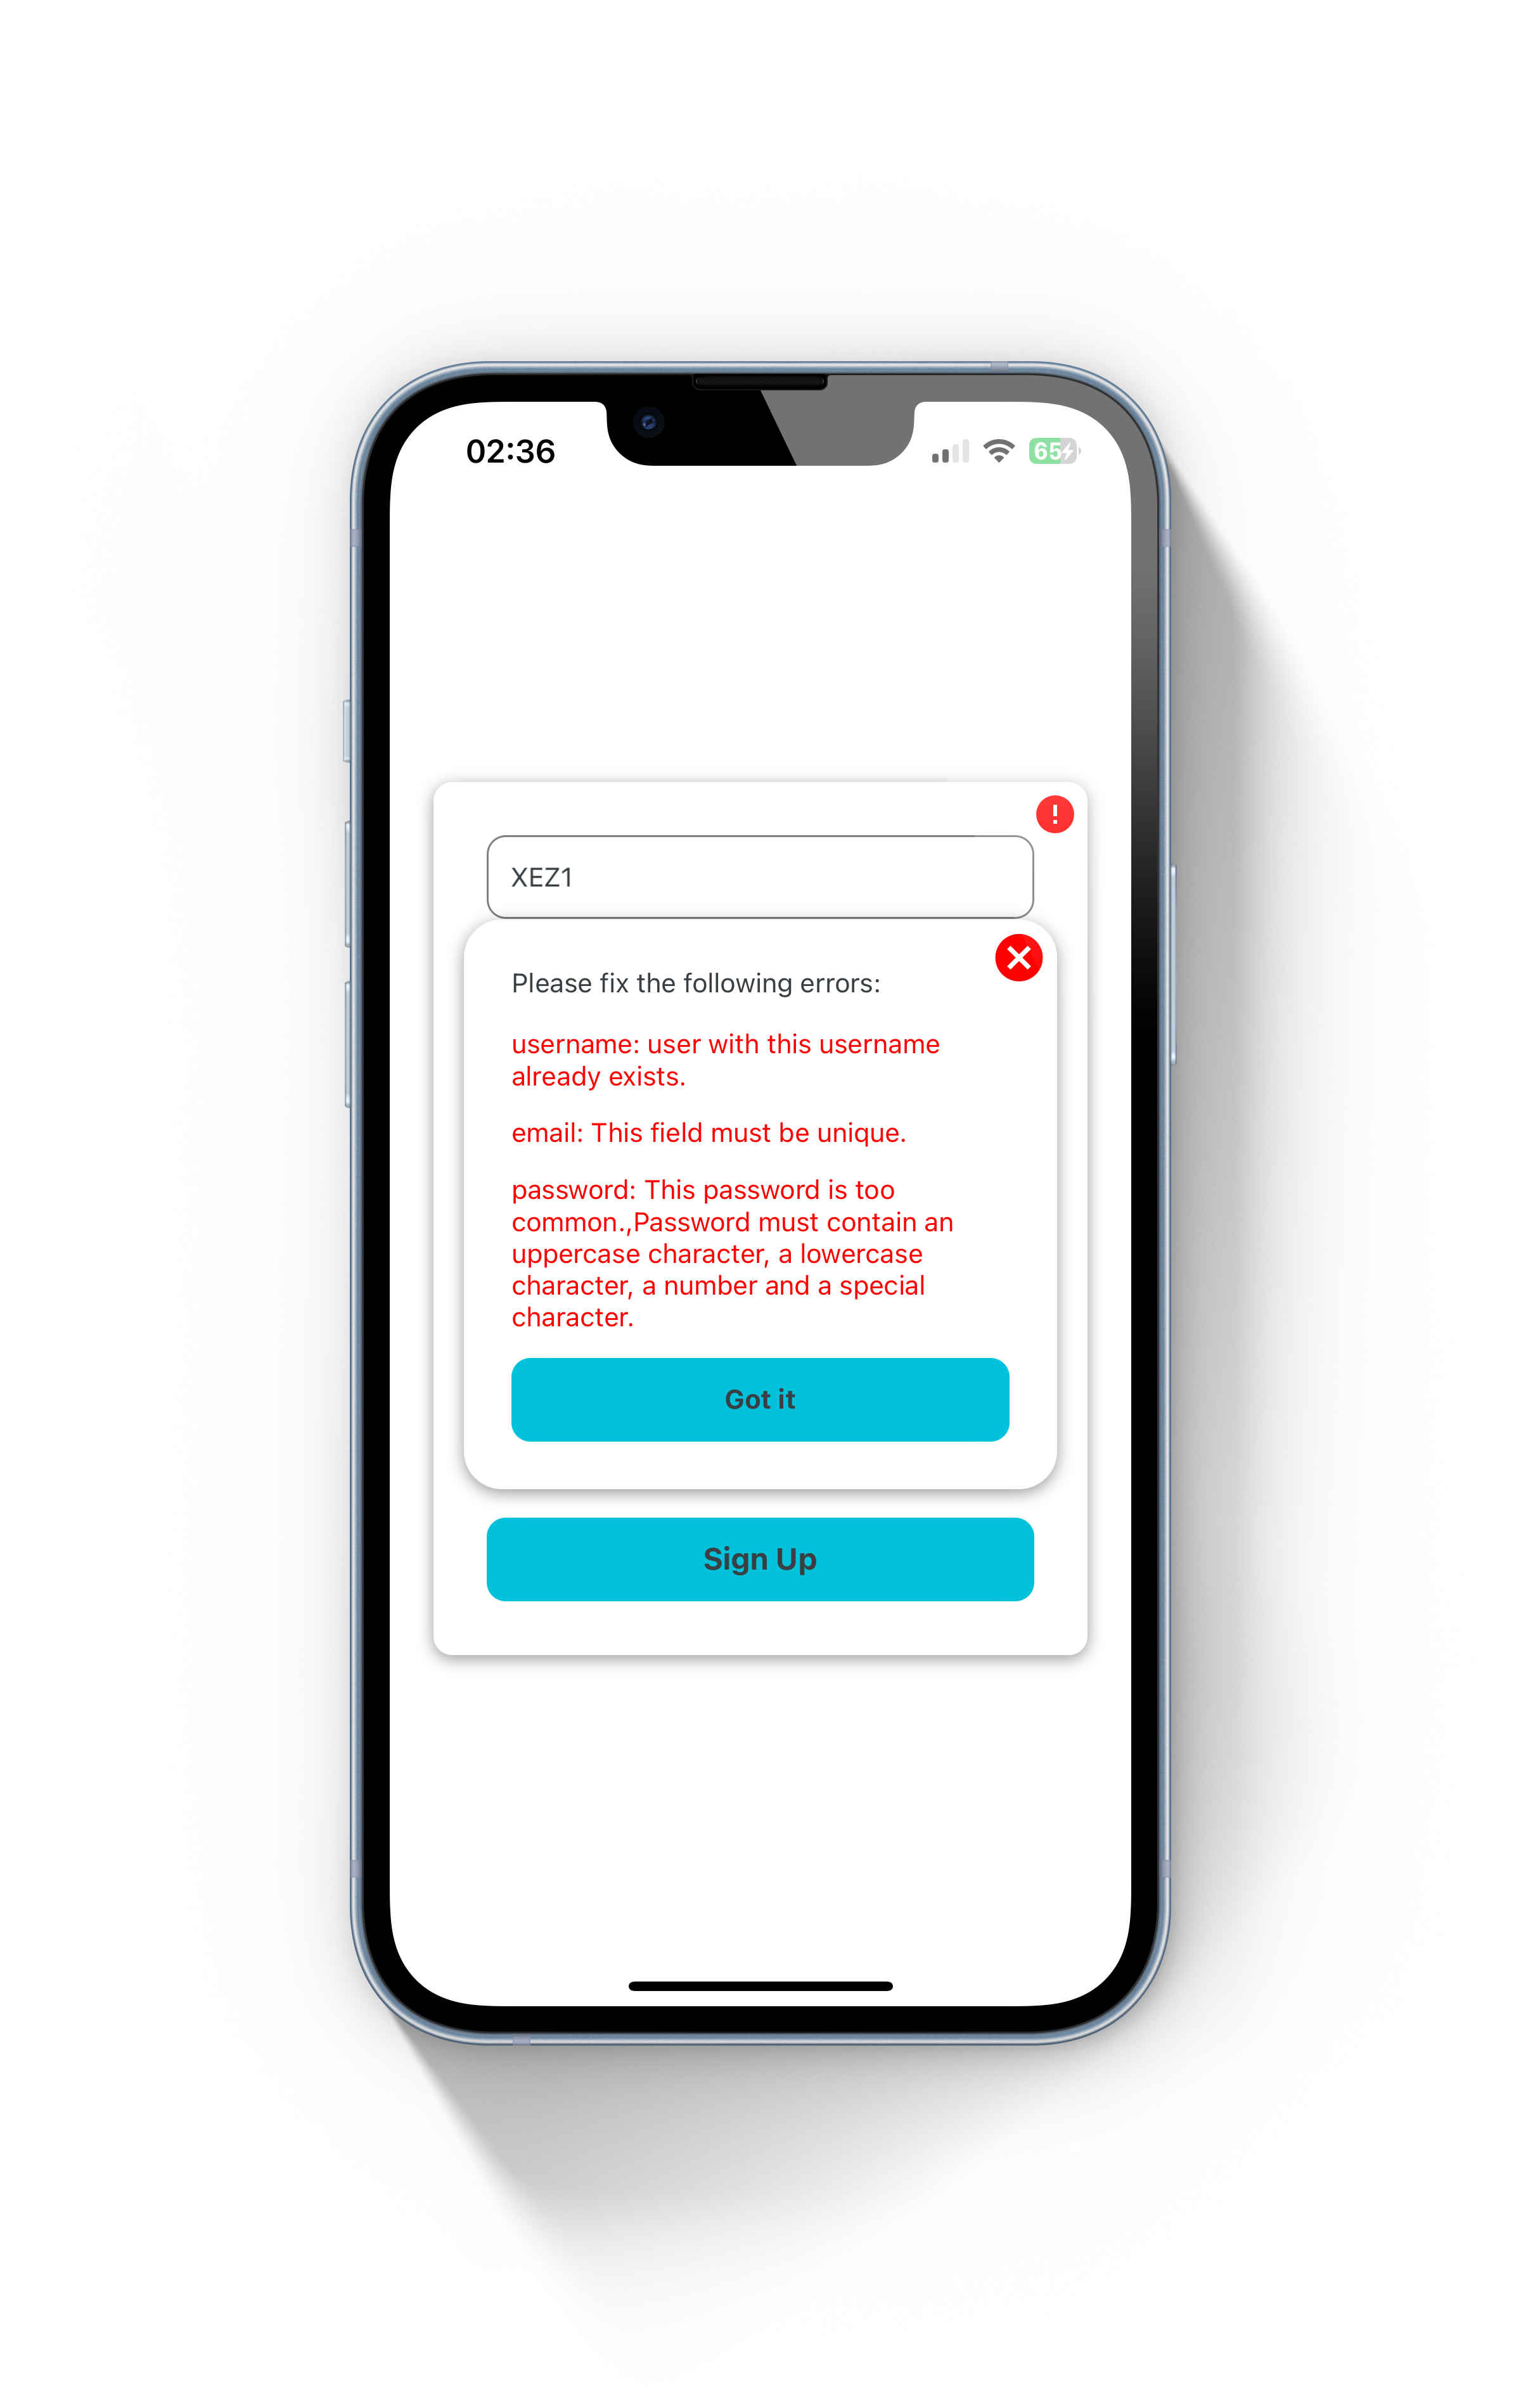
\includegraphics[scale=0.1]{LATEX/Appendices/Images/Software/Frontend/sign_up_screen_2.png}
        \caption{Sign Up Screen 2 Appearance}
        \label{fig:sign up screen 2}
        \end{minipage}
\end{figure}

\subsubsection{PostLoginScreens: HomeScreen.js}

This screen includes sections for building smart contracts, displaying saved contracts, and performing address checksum conversions.

\begin{figure}[!ht]
    \centering
    % Begin the first minipage for the first image
    \begin{minipage}{0.49\textwidth}
        \centering
        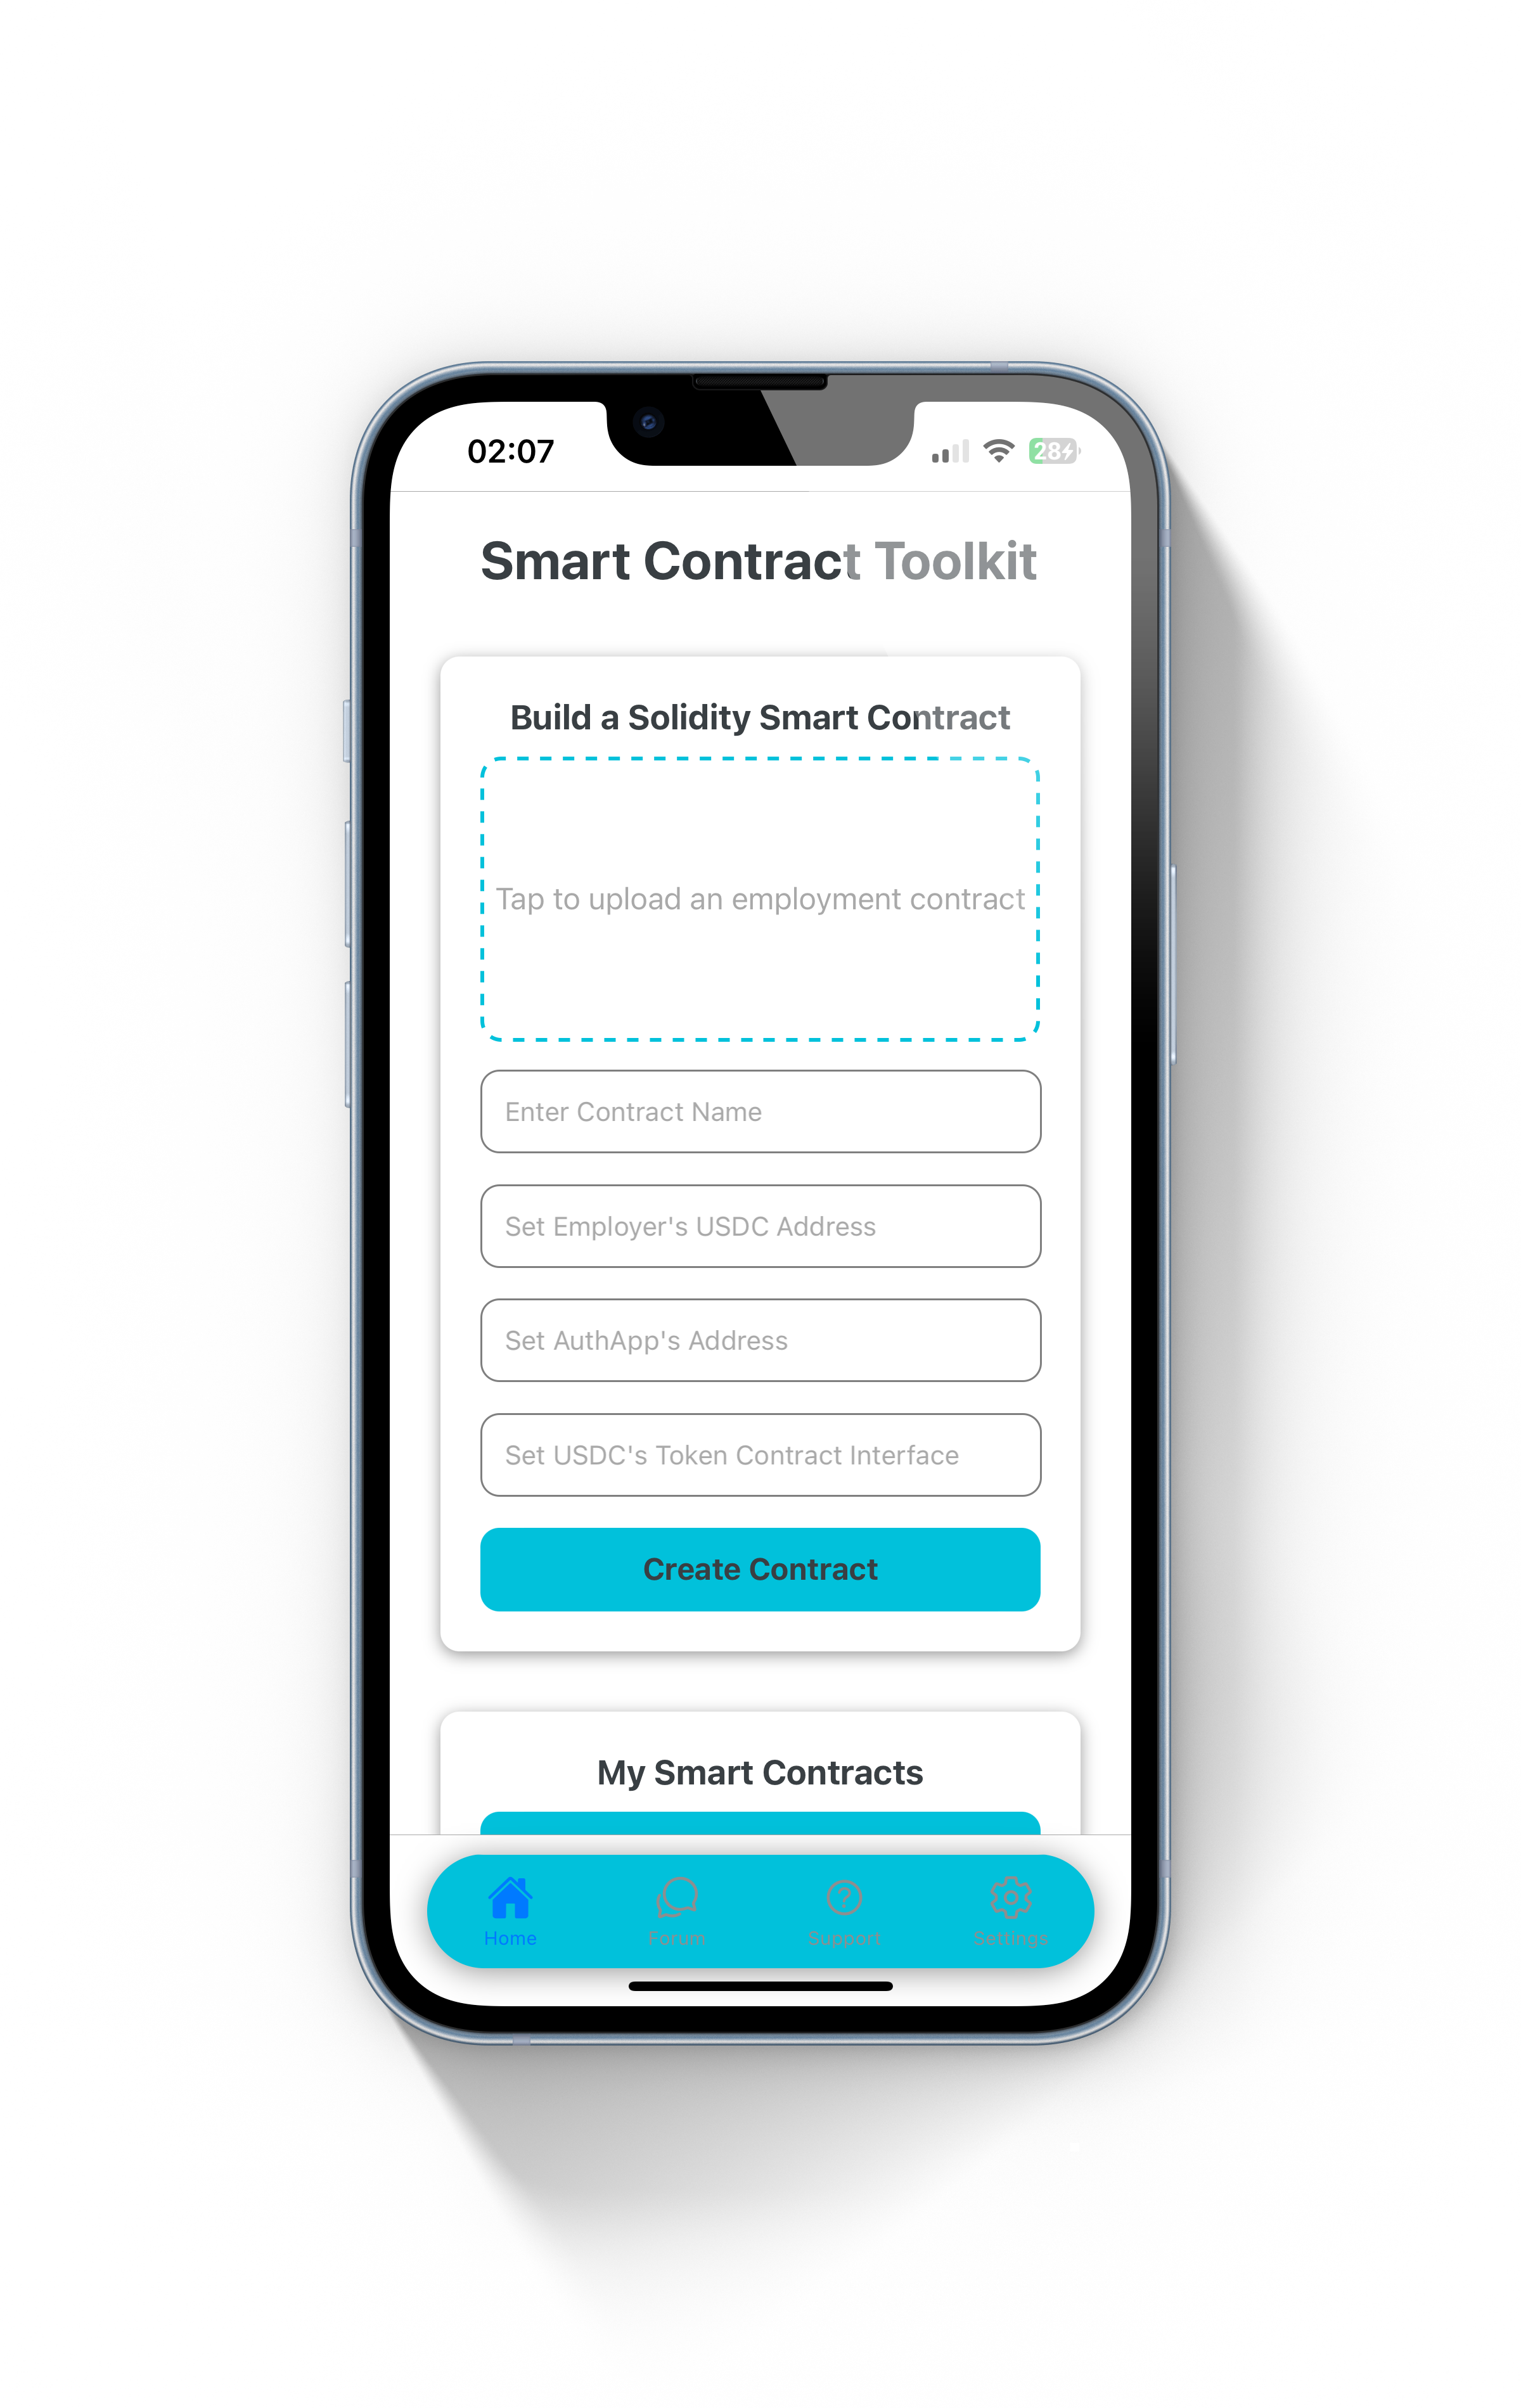
\includegraphics[scale=0.07]{LATEX/Appendices/Images/Software/Frontend/home_screen_1.png}
        \caption{Home Screen (Upper Part) Appearance}
        \label{fig:home screen 1}
    \end{minipage}\hfill % This inserts a small horizontal space between the minipages
    % Begin the second minipage for the second image
    \begin{minipage}{0.49\textwidth}
        \centering
        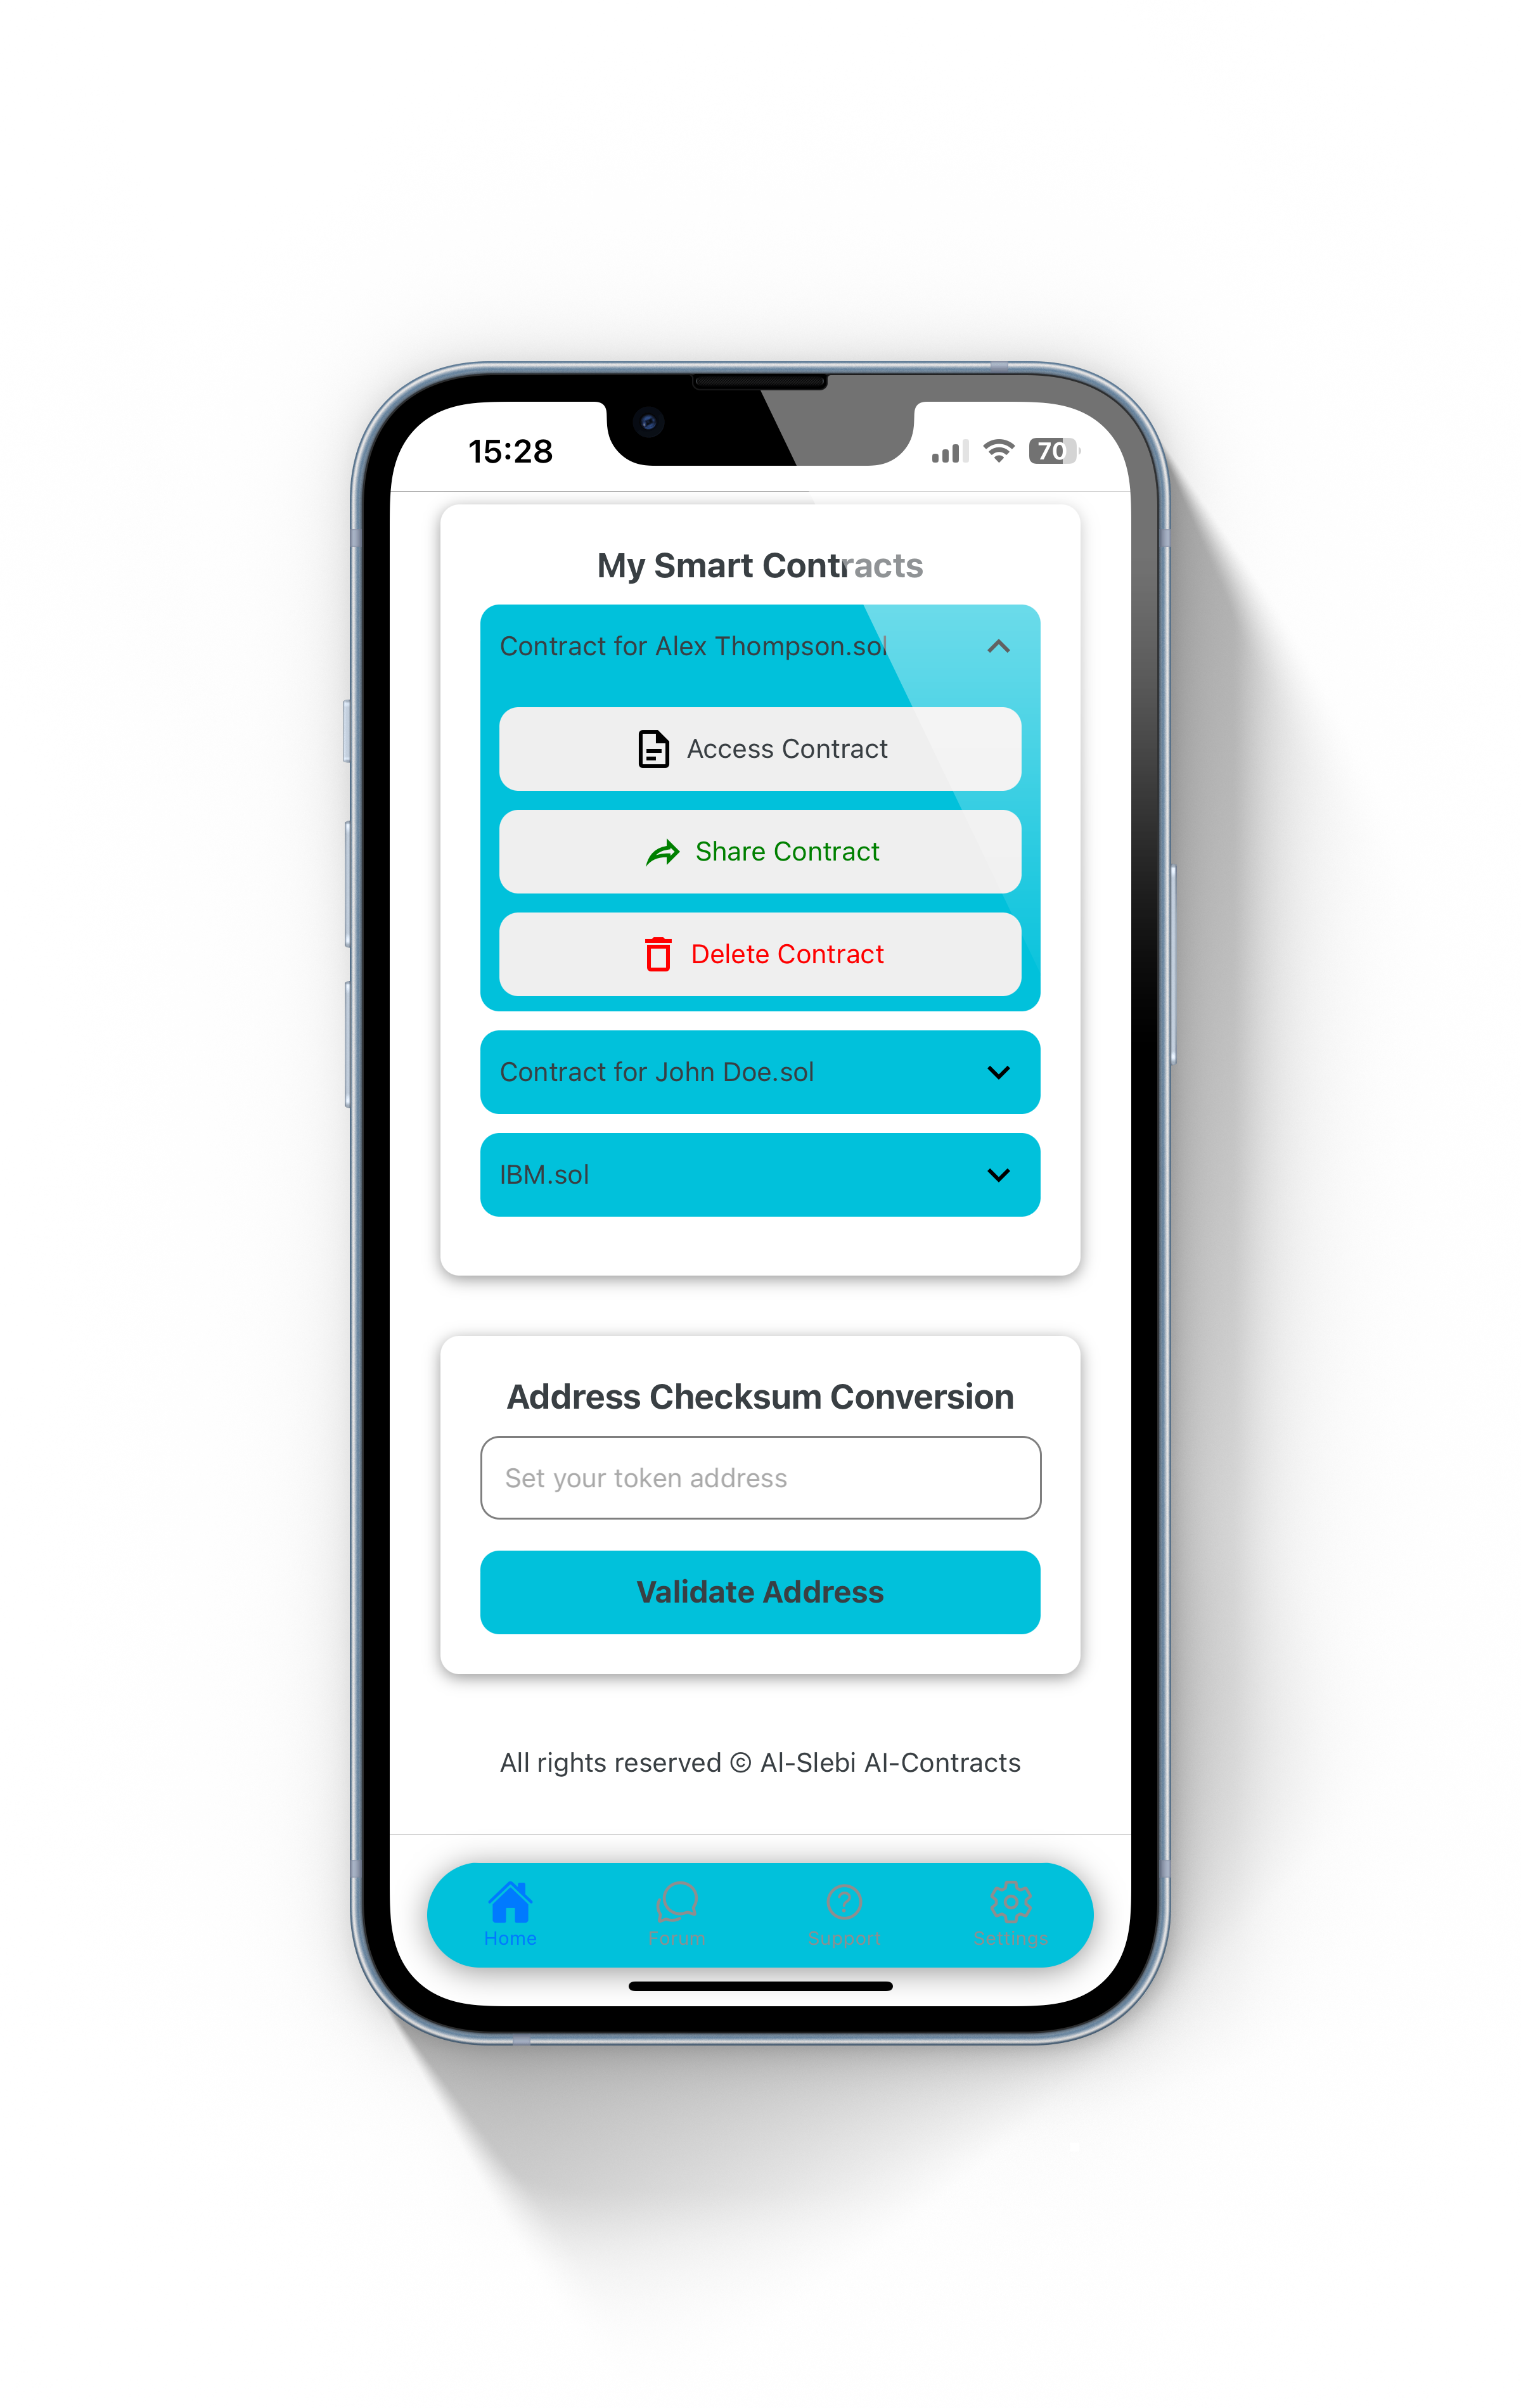
\includegraphics[scale=0.07]{LATEX/Appendices/Images/Software/Frontend/home_screen_2.png}
        \caption{Home Screen (Bottom Part) Appearance}
        \label{fig:home screen 2}
    \end{minipage}
\end{figure}

\begin{figure}[!ht]
    \centering
    % Begin the first minipage for the first image
    \begin{minipage}{0.49\textwidth}
        \centering
        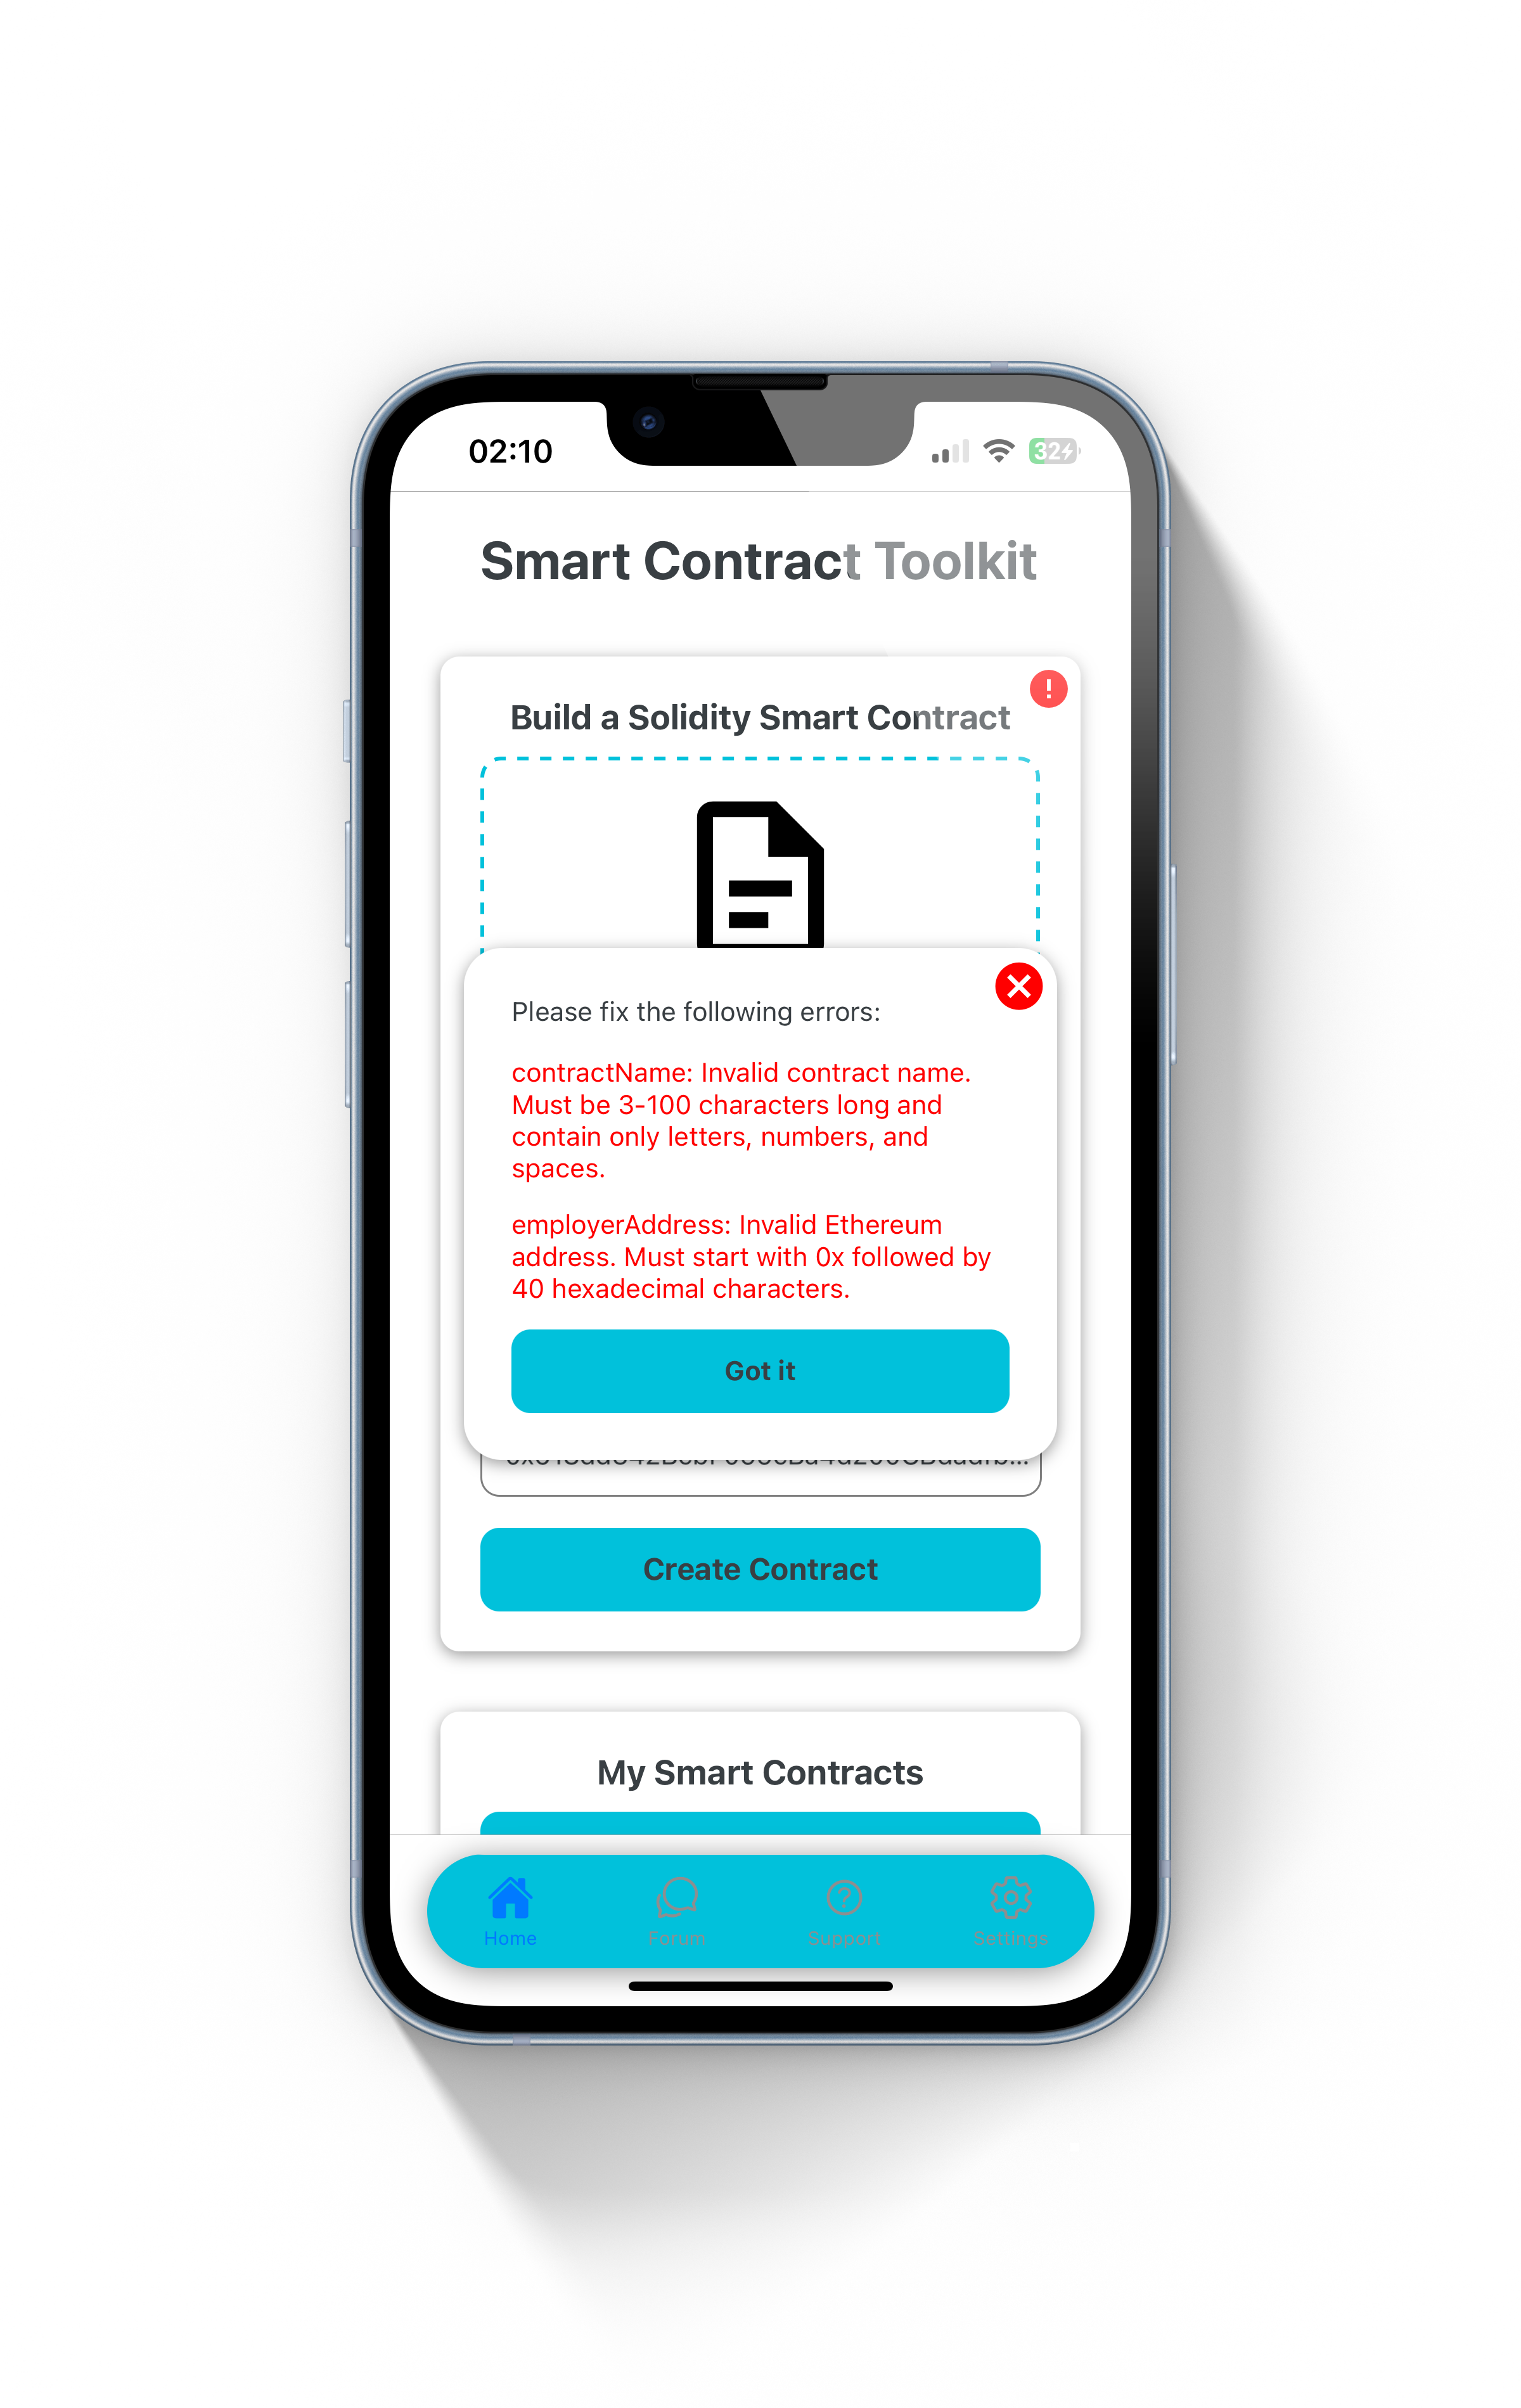
\includegraphics[scale=0.07]{LATEX/Appendices/Images/Software/Frontend/home_screen_3.png}
        \caption{Home Screen (Error Modal on Contract Update) Appearance}
        \label{fig:home screen 3}
    \end{minipage}\hfill % This inserts a small horizontal space between the minipages
    % Begin the second minipage for the second image
    \begin{minipage}{0.49\textwidth}
        \centering
        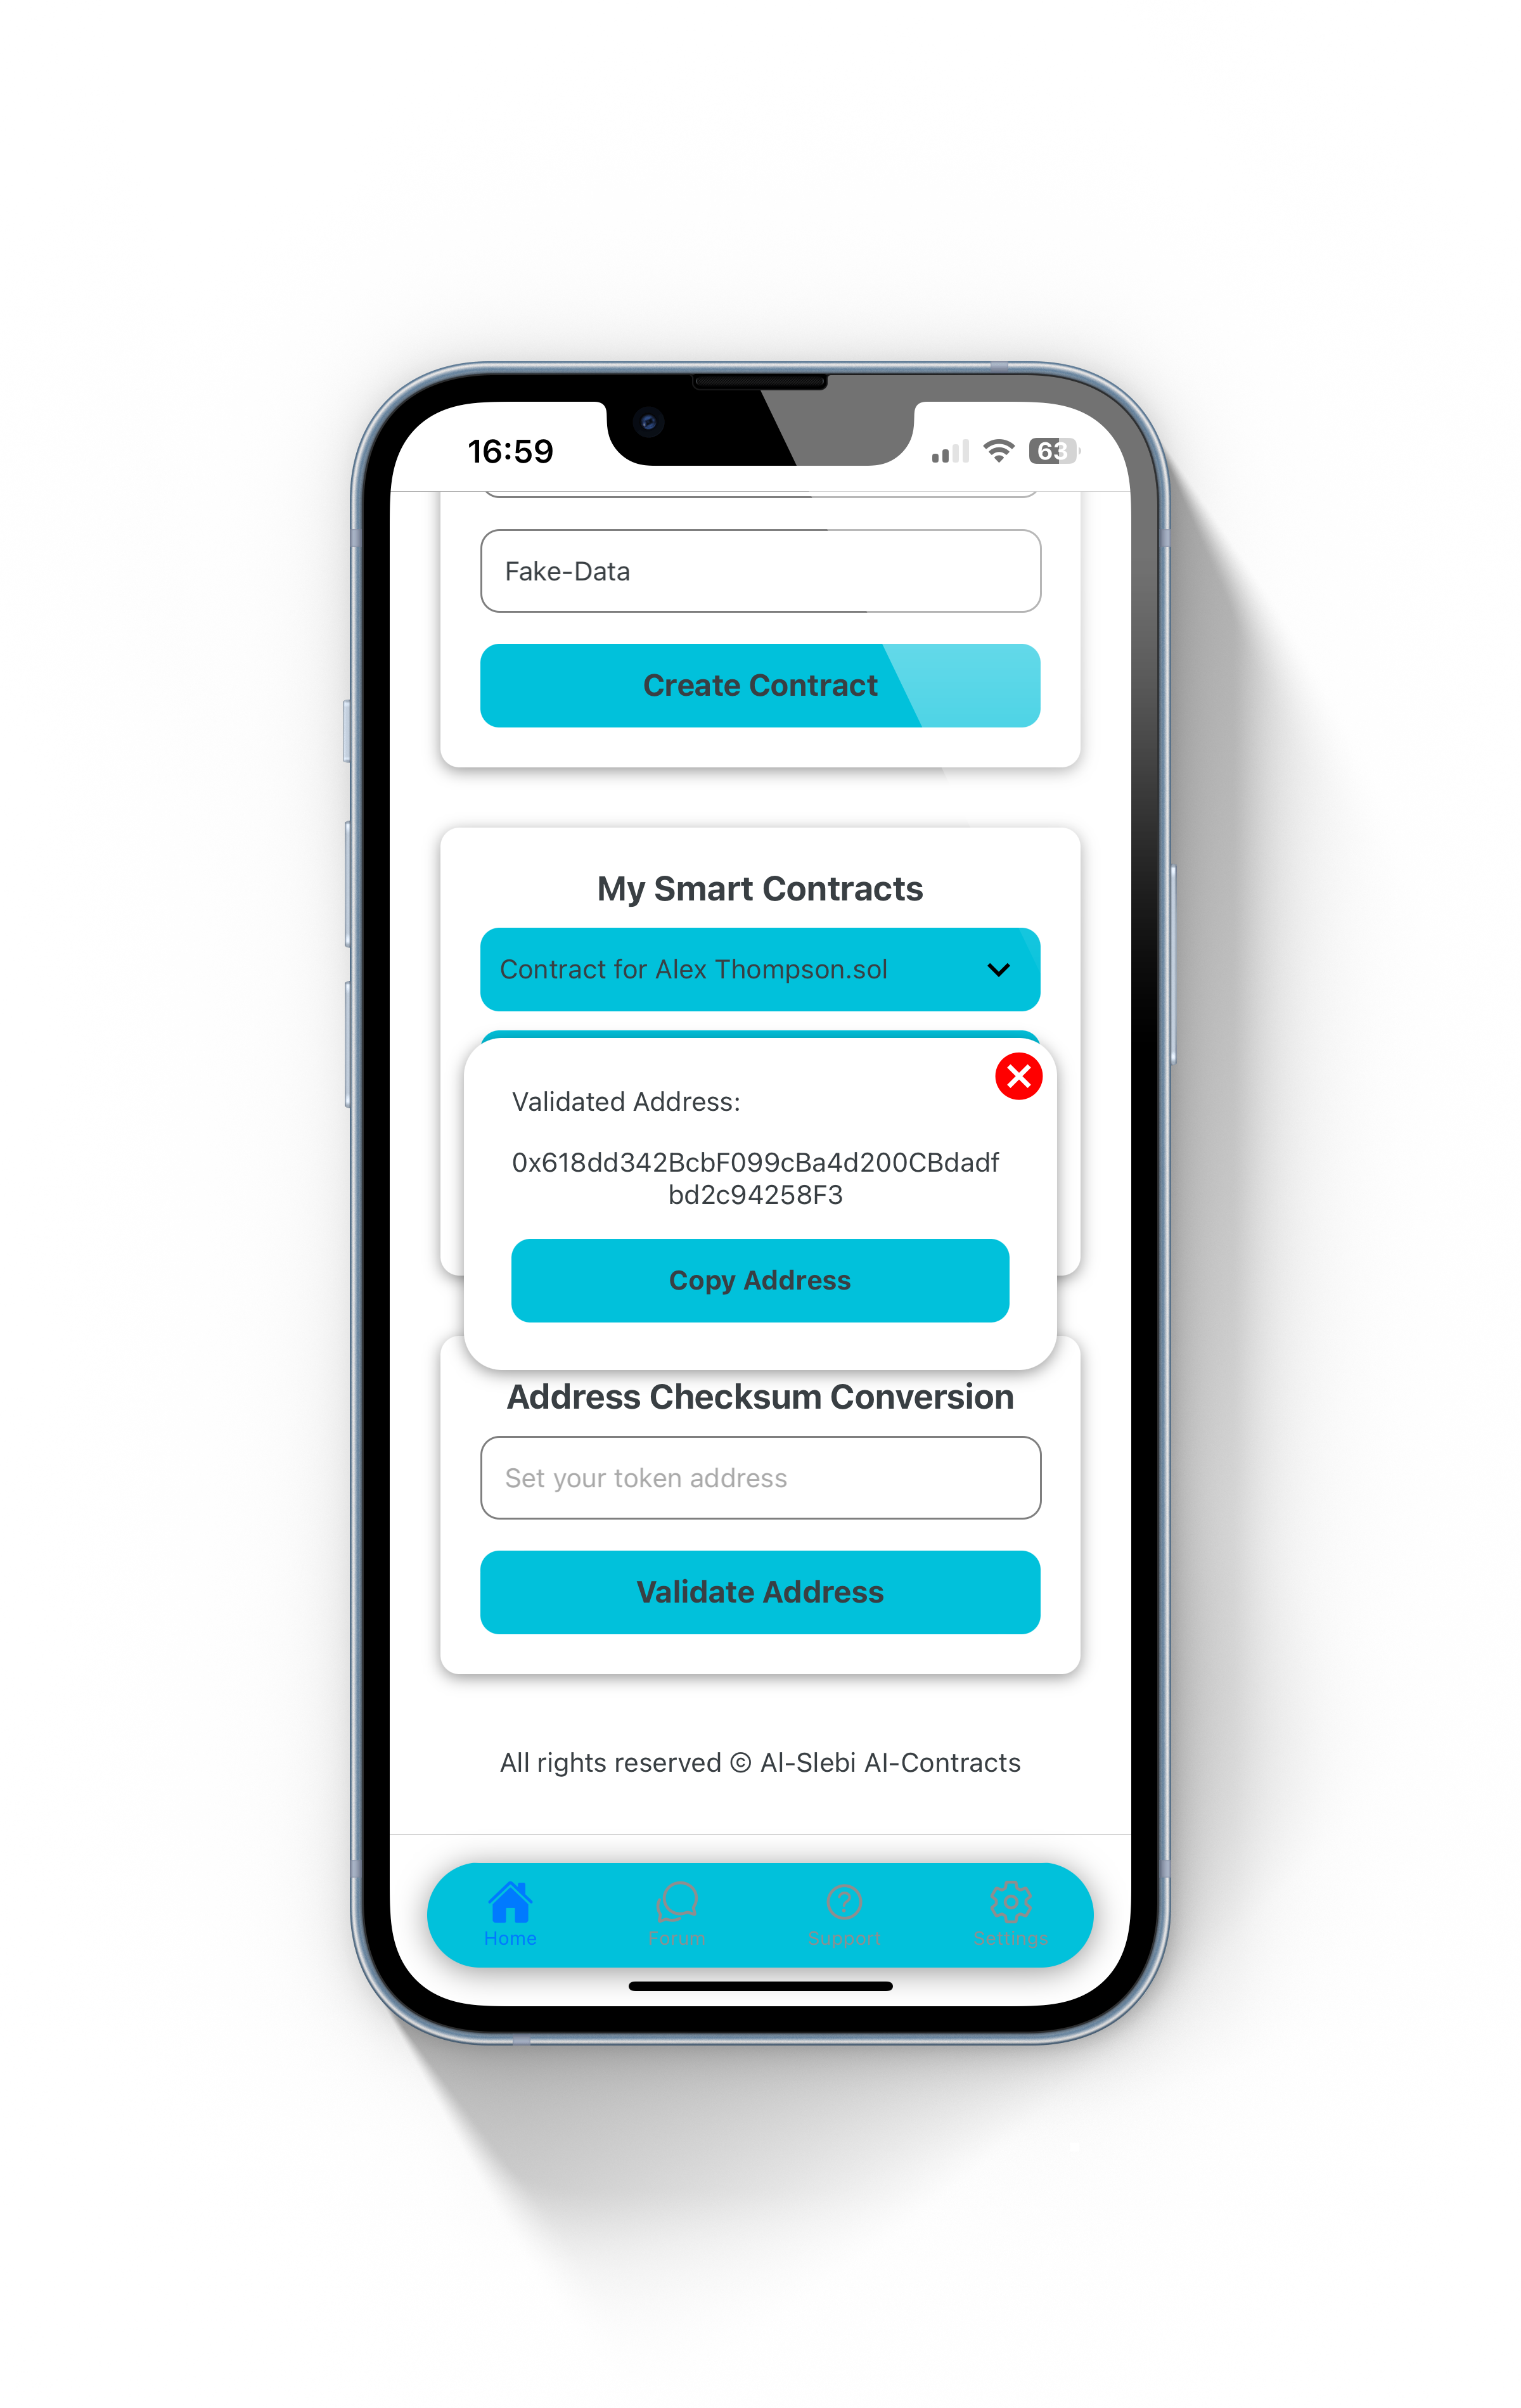
\includegraphics[scale=0.07]{LATEX/Appendices/Images/Software/Frontend/home_screen_4.png}
        \caption{Home Screen (Modal on Address Checksum Conversion) Appearance}
        \label{fig:home screen 4}
    \end{minipage}
\end{figure}

The \texttt{HomeScreen} functional component handles the rendering of the home screen. Within this component:

\begin{itemize}
    \item State variables and functions for managing contract data, user input validation, file selection, contract operations, errors, and modal visibility are retrieved from the \texttt{useHomeScreen} custom hook. This hook is responsible for the animations and all backend interactions on the home screen.
    \item The \textit{useEffect} hook is used to fetch and synchronise contracts when the component mounts.
\end{itemize}

The component returns a view hierarchy structured as follows:

\begin{itemize}
    \item A main \textit{View} container adjusted based on the keyboard height.
    \item A \textit{ScrollView} for overflow content. It is referenced to manage keyboard interactions.
    \item Inside the \textit{ScrollView}, a nested \textit{View} component contains:
    \begin{itemize}
        \item A header label for the page.
        \item A Contract creation section, styled as a card, with:
        \begin{itemize}
            \item An error icon and modal for displaying input validation errors.
            \item A card header for the contract creation section.
            \item A \textit{TouchableOpacity} component serving as a drop zone for file uploads.
            \item Multiple \textit{TextInput} components for entering contract details.
            \item A \textit{TouchableOpacity} component acting as the "Create Contract" button.
        \end{itemize}
        \item A card section for displaying the user's saved contracts, which includes:
        \begin{itemize}
            \item A card header for the saved contracts section.
            \item A list of \textit{ContractItem} components for each saved contract.
            \item A message in a visually appealing box indicating if there are no saved contracts.
        \end{itemize}
        \item A card section for address checksum conversion, which includes:
        \begin{itemize}
            \item A card header for the address checksum conversion section.
            \item A \textit{TextInput} component for entering the token address.
            \item A \textit{TouchableOpacity} component acting as the "Validate Address" button.
            \item A modal for displaying the validated address and providing options to copy or close the modal.
        \end{itemize}
        \item A footer section with copyright information.
    \end{itemize}
    \item A separator line at the bottom, with its position adjusted based on the keyboard height.
\end{itemize}

\subsubsection{PostLoginScreens: UseHomeScreen.js}

The file defines the \texttt{useHomeScreen} custom hook, which is used to control the \textit{HomeScreen} component's functionality and state.

\begin{itemize}
    \item \textbf{State Variables:}
    \begin{itemize}
        \item \textit{selectedFile} manages the state of the selected file for contract creation.
        \item \textit{contractName}, \textit{employerAddress}, \textit{authAppAddress}, and \textit{tokenContractInterface} store user inputs for contract details.
        \item Contracts stored on the device are tracked by the \textit{savedContracts} variable.
        \item \textit{isComponentMounted} is a flag to check if the component is mounted.
        \item \textit{showAddressModal} and \textit{validatedAddress} manage the state for displaying and storing the validated Ethereum address.
        \item \textit{errors} and \textit{showErrorDetails} handle validation errors and their visibility.
        \item The Ethereum address that users input to be validated is stored by \textit{addressChecksum} variable.
    \end{itemize}

    \item \textbf{File Selection:}
    \begin{itemize}
        \item Using \textit{ExpoDocumentPicker}, \textit{handleFileSelectDropZone} enables users to choose a file for contract generation. It determines whether the file selection has been cancelled and modifies the \textit{selectedFile} state as necessary. By using \textit{LayoutAnimation}, it also controls the component's animation.
        \begin{itemize}
            \item If the file selection is cancelled and a file is already selected, it clears the \textit{selectedFile} state.
            \item If the file is of type \textit{``text/plain''}, it sets the \textit{selectedFile} state with its details.
        \end{itemize}
    \end{itemize}

    \item \textbf{Upload Contract Data:}
    \begin{itemize}
        \item The function \textit{uploadContractData} is responsible for managing the uploading of contract data. It validates input and verifies that the file and all required fields are supplied. By using \textit{LayoutAnimation}, it also controls the component's animation.
        \item It reads the file content using \textit{FileSystem.readAsStringAsync}, prepares \textit{FormData}, and sends it to the backend server using a \textit{POST} request.
        \item It notifies the user and resets the input fields upon a successful upload.
    \end{itemize}

    \item \textbf{Save Solidity File:}
    \begin{itemize}
        \item \textit{saveSolidityFile} saves the generated Solidity code to the device's file system and controls the animation through \textit{LayoutAnimation}.
        \begin{itemize}
            \item Checks if the file already exists using \textit{FileSystem.getInfoAsync} and overwrites it if necessary.
            \item Saves the file using \textit{FileSystem.writeAsStringAsync}, updates the \textit{savedContracts} state, and alerts the user.
        \end{itemize}
    \end{itemize}

    \item \textbf{Share Contract:}
    \begin{itemize}
        \item \textit{ShareContract} enables users to use \textit{expo-sharing} library to distribute the created contract files. It transmits the file path after determining whether the device possesses the right permission. According to the convention, other applications retrieve the document accordingly from the phone's file system (based on the convention).
    \end{itemize}

    \item \textbf{Open Contract:}
    \begin{itemize}
        \item \textit{openContract} navigates the user to the \textit{EditorScreen} with the path of the selected contract file.
    \end{itemize}

    \item \textbf{Fetch and Sync Contracts:}
    \begin{itemize}
        \item Contracts that have been saved by the user are retrieved from the backend server and synchronised with the local file system using the \textit{fetchAndSyncContracts} function.
        \item It uses the \textit{syncContracts} function to ensure that all contracts are downloaded and saved locally if they do not already exist.
    \end{itemize}

    \item \textbf{Sync Contracts:}
    \begin{itemize}
        \item \textit{syncContracts} iterates over the fetched contracts and saves them locally if they are not already present in the device's file system.
        \begin{itemize}
            \item It uses \textit{FileSystem.readDirectoryAsync} to read the local directory and verify that every contract pulled from the backend is present there.
            \item If a contract is not found locally, it downloads and saves the contract using \textit{saveSolidityFile}.
        \end{itemize}
    \end{itemize}

    \item \textbf{Delete Contract:}
    \begin{itemize}
        \item \textit{handleDeleteContract} deletes a contract both locally and on the backend server, simulating an animation through \textit{LayoutAnimation}.
        \begin{itemize}
            \item It sends a \textit{DELETE} request to the backend server and deletes the local file using \textit{FileSystem.deleteAsync}.
            \item Updates the \textit{savedContracts} state to reflect the deletion.
        \end{itemize}
    \end{itemize}

    \item \textbf{Clean Expo Folder:}
    \begin{itemize}
        \item \textit{cleanExpoFolder} deletes all files in the Expo document directory.
        \begin{itemize}
            \item It reads the directory using \textit{FileSystem.readDirectoryAsync} and deletes each file using \textit{FileSystem.deleteAsync}.
        \end{itemize}
    \end{itemize}

    \item \textbf{Input Validation:}
    \begin{itemize}
        \item \textit{validateInput} is a helper method that updates the state of \textit{errors} variable through the output of the \textit{getValidationErrorMessage} function.
        \item \textit{getValidationErrorMessage} returns appropriate error messages by validating Ethereum addresses, contract names, and JSON formats.
    \end{itemize}

    \item \textbf{Handle Checksum Address:}
    \begin{itemize}
        \item \textit{handleChecksumAddress} validates an Ethereum address by sending a \textit{GET} request to the backend server.
        \begin{itemize}
            \item If the address is valid, it sets the \textit{validatedAddress} state and displays the address in a modal.
            \item If the address is invalid, it displays an error alert.
        \end{itemize}
    \end{itemize}

    \item \textbf{Copy to Clipboard:}
    \begin{itemize}
        \item \textit{copyToClipboard} copies the validated Ethereum address to the clipboard and alerts the user.
    \end{itemize}

    \item \textbf{Additional Helper Functions:}
    \begin{itemize}
        \item \textit{isValidEthereumAddress}, \textit{isValidHexadecimal}, \textit{isValidContractName}, \textit{isValidJson}, and \textit{getValidationErrorMessage} are helper functions used for validating user inputs.
    \end{itemize}
\end{itemize}

In summary, the \textit{useHomeScreen} custom hook simplifies and modularises the code by encapsulating the state management and necessary functionalities needed for the \textit{HomeScreen} UI component.

\subsubsection{PostLoginScreens: ContractItem.js}

Users can open, share, delete, and expand contract details through this component. 

\begin{itemize}
    \item \textbf{State Variables and Refs:}
    \begin{itemize}
        \item \textit{expanded}: A state variable to track whether the contract details are expanded or collapsed.
        \item \textit{animationController}: An animated value to control the height of the contract details section.
        \item \textit{opacityAnimation} and \textit{heightAnimation}: During deletion, the opacity and height are controlled by these states.
        \item \textit{isMounted}: A reference for detecting animations and halting them.
    \end{itemize}

    \item \textbf{useEffect Hook:}
    \begin{itemize}
        \item The \textit{useEffect} hook sets \textit{isMounted} to \textit{false} and stops the animation controller when the component unmounts.
    \end{itemize}

    \item \textbf{toggleExpand:}
    \begin{itemize}
        \item This function initiates an animation to expand or compress the details section. It also refreshes the expanded state.
        \item Uses \textit{Animated.timing} to animate the \textit{animationController} value over 500 milliseconds.
    \end{itemize}

    \item \textbf{initiateDeletion:}
    \begin{itemize}
        \item This method shows an alert to confirm the deletion of a contract.
        \item If the user confirms, it triggers the \texttt{handleDeletionAnimation}.
    \end{itemize}

    \item \textbf{handleDeletionAnimation:}
    \begin{itemize}
        \item It performs an animation to fade out and collapse the contract item before deleting it.
        \item Uses \textit{Animated.parallel} to run the opacity and height animations simultaneously over 300 milliseconds.
        \item Calls the \textit{deleteContract} function to remove the contract after the animation completes.
    \end{itemize}

    \item \textbf{animatedHeight:}
    \begin{itemize}
        \item This interpolates the \textit{animationController} value to animate the height of the contract details section between 0 and 180 pixels.
    \end{itemize}

    \item \textbf{Return Statement:}
    \begin{itemize}
        \item The \textit{ContractItem} component renders a \textit{TouchableOpacity} container that toggles the expansion of the contract details.
        \item It displays the contract name and an icon indicating the expanded state.
        \item The animated view expands to show additional actions: \textit{Access Contract}, \textit{Share Contract}, and \textit{Delete Contract}.
    \end{itemize}
\end{itemize}

\subsubsection{PostLoginScreens: EditorScreen.js}

\begin{figure}[!ht]
    \centering
    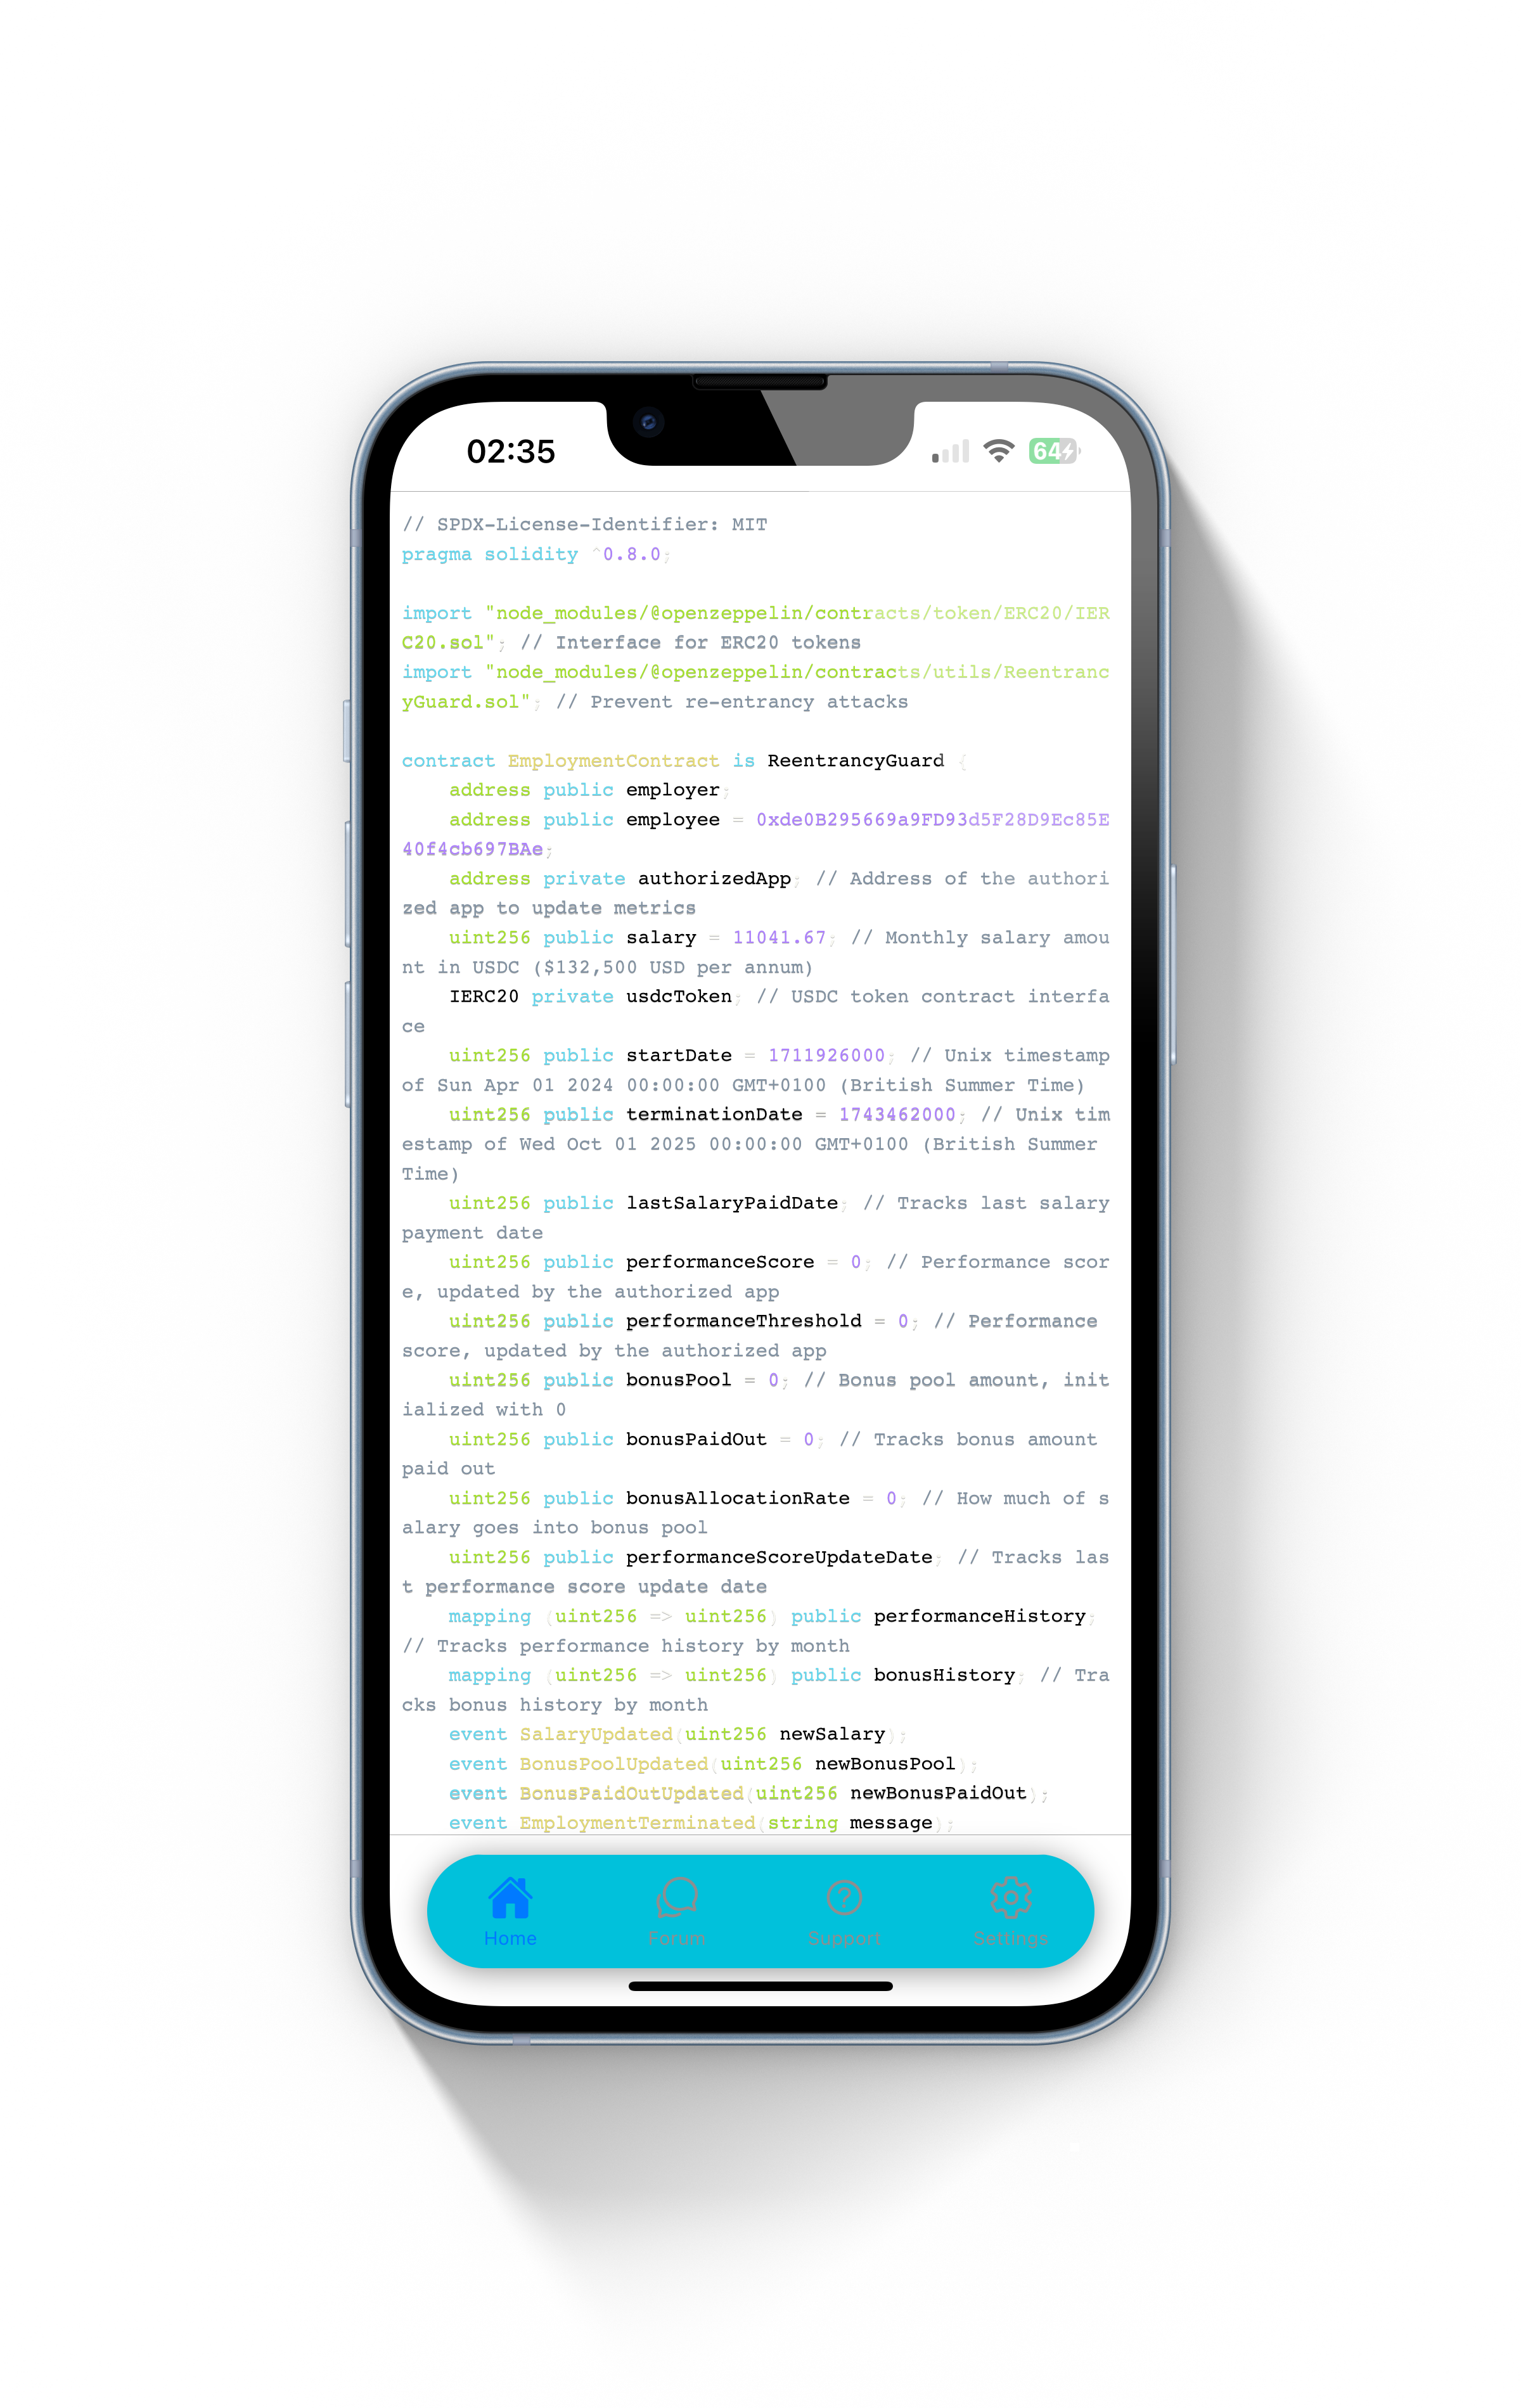
\includegraphics[width=0.5\textwidth]
    {LATEX/Appendices/Images/Software/Frontend/editor_screen.png}
    \caption{Editor Screen Appearance}
    \label{fig:editor screen}
\end{figure}

The \texttt{EditorScreen} is a functional component that uses \textit{navigation} and \textit{route} as props.

\begin{itemize}
    \item \textbf{Parameters and Hook:}
    \begin{itemize}
        \item The file path of the contract to be edited is retrieved from \textit{route.params}.
        \item The custom hook \textit{useEditorScreen} is called with the file path and theme as arguments to fetch the HTML content of the code and the loading state.
    \end{itemize}

    \item \textbf{Return Statement:}
    \begin{itemize}
        \item A view container with conditional rendering based on the \textit{isLoading} state is returned by the component.
        \begin{itemize}
            \item If \textit{isLoading} is true, an \textit{ActivityIndicator} is displayed.
            \item If \textit{isLoading} is false, a \textit{WebView} component is rendered to display the HTML content of the code.
        \end{itemize}
        \item The \textit{WebView} component uses \textit{originWhitelist} to allow all origins and sets the source to the HTML content obtained from the custom hook.
        \item The \textit{WebView} and \textit{ActivityIndicator} are styled using the shared and local styles.
        
        \item A separator line is included at the bottom using the \textit{sharedStyles.separatorLine}.
    \end{itemize}
\end{itemize}

\subsubsection{PostLoginScreens: UseEditorScreen.js}

A customised hook that loads and formats contract file content for \textit{web view} presentation is defined in the \texttt{UseEditorScreen.js} file

\begin{itemize}
    \item \textbf{State Variables:}
    \begin{itemize}
        \item \textit{fileContent}: Stores the raw content of the contract file.
        \item \textit{codeHtml}: Stores the HTML content generated from the raw contract file.
        \item \textit{isLoading}: A boolean flag indicating whether the file content is still loading.
    \end{itemize}

    \item \textbf{useEffect Hook for Loading File Content:}
    \begin{itemize}
        \item The first \textit{useEffect} hook is responsible for loading the content of the contract file specified by \textit{filePath}.
        \item It defines an asynchronous function, \textit{loadFileContent}, which reads the file content using \textit{FileSystem.readAsStringAsync}.
        \item The file content is then stored in the \textit{fileContent} state variable.
        \item If an error occurs during file reading, an alert is displayed, and the error is logged to the console.
    \end{itemize}

    \item \textbf{useEffect Hook for Generating HTML Content:}
    \begin{itemize}
        \item The second \textit{useEffect} hook is responsible for generating the HTML content from the raw file.
        \item It runs whenever the \textit{theme} or \textit{fileContent} changes.
        \item The file content is escaped to prevent HTML injection by replacing special characters with their corresponding HTML entities.
        \item An HTML template is created, which includes:
        \begin{itemize}
            \item A link to the Prism CSS file for syntax highlighting.
            \item Scripts for \textit{Prism} and \textit{Solidity} syntax highlighting.
            \item Inline styles for setting the background and text colours, font properties, and ensuring proper word wrapping and formatting.
        \end{itemize}
        \item The escaped content is embedded within a \textit{<pre><code>} block for syntax highlighting.
        \item The generated HTML template is stored in the \textit{codeHtml} state variable.
        \item The \textit{isLoading} state is set to \textit{false}.
    \end{itemize}

    \item \textbf{Return Values:}
    \begin{itemize}
        \item The hook returns the \textit{codeHtml} and \textit{isLoading} values, which are used by the \textit{EditorScreen} component to display the contract code.
    \end{itemize}
\end{itemize}

\subsubsection{PostLoginScreens: ForumScreen.js}

\begin{figure}[!ht]
    \centering
    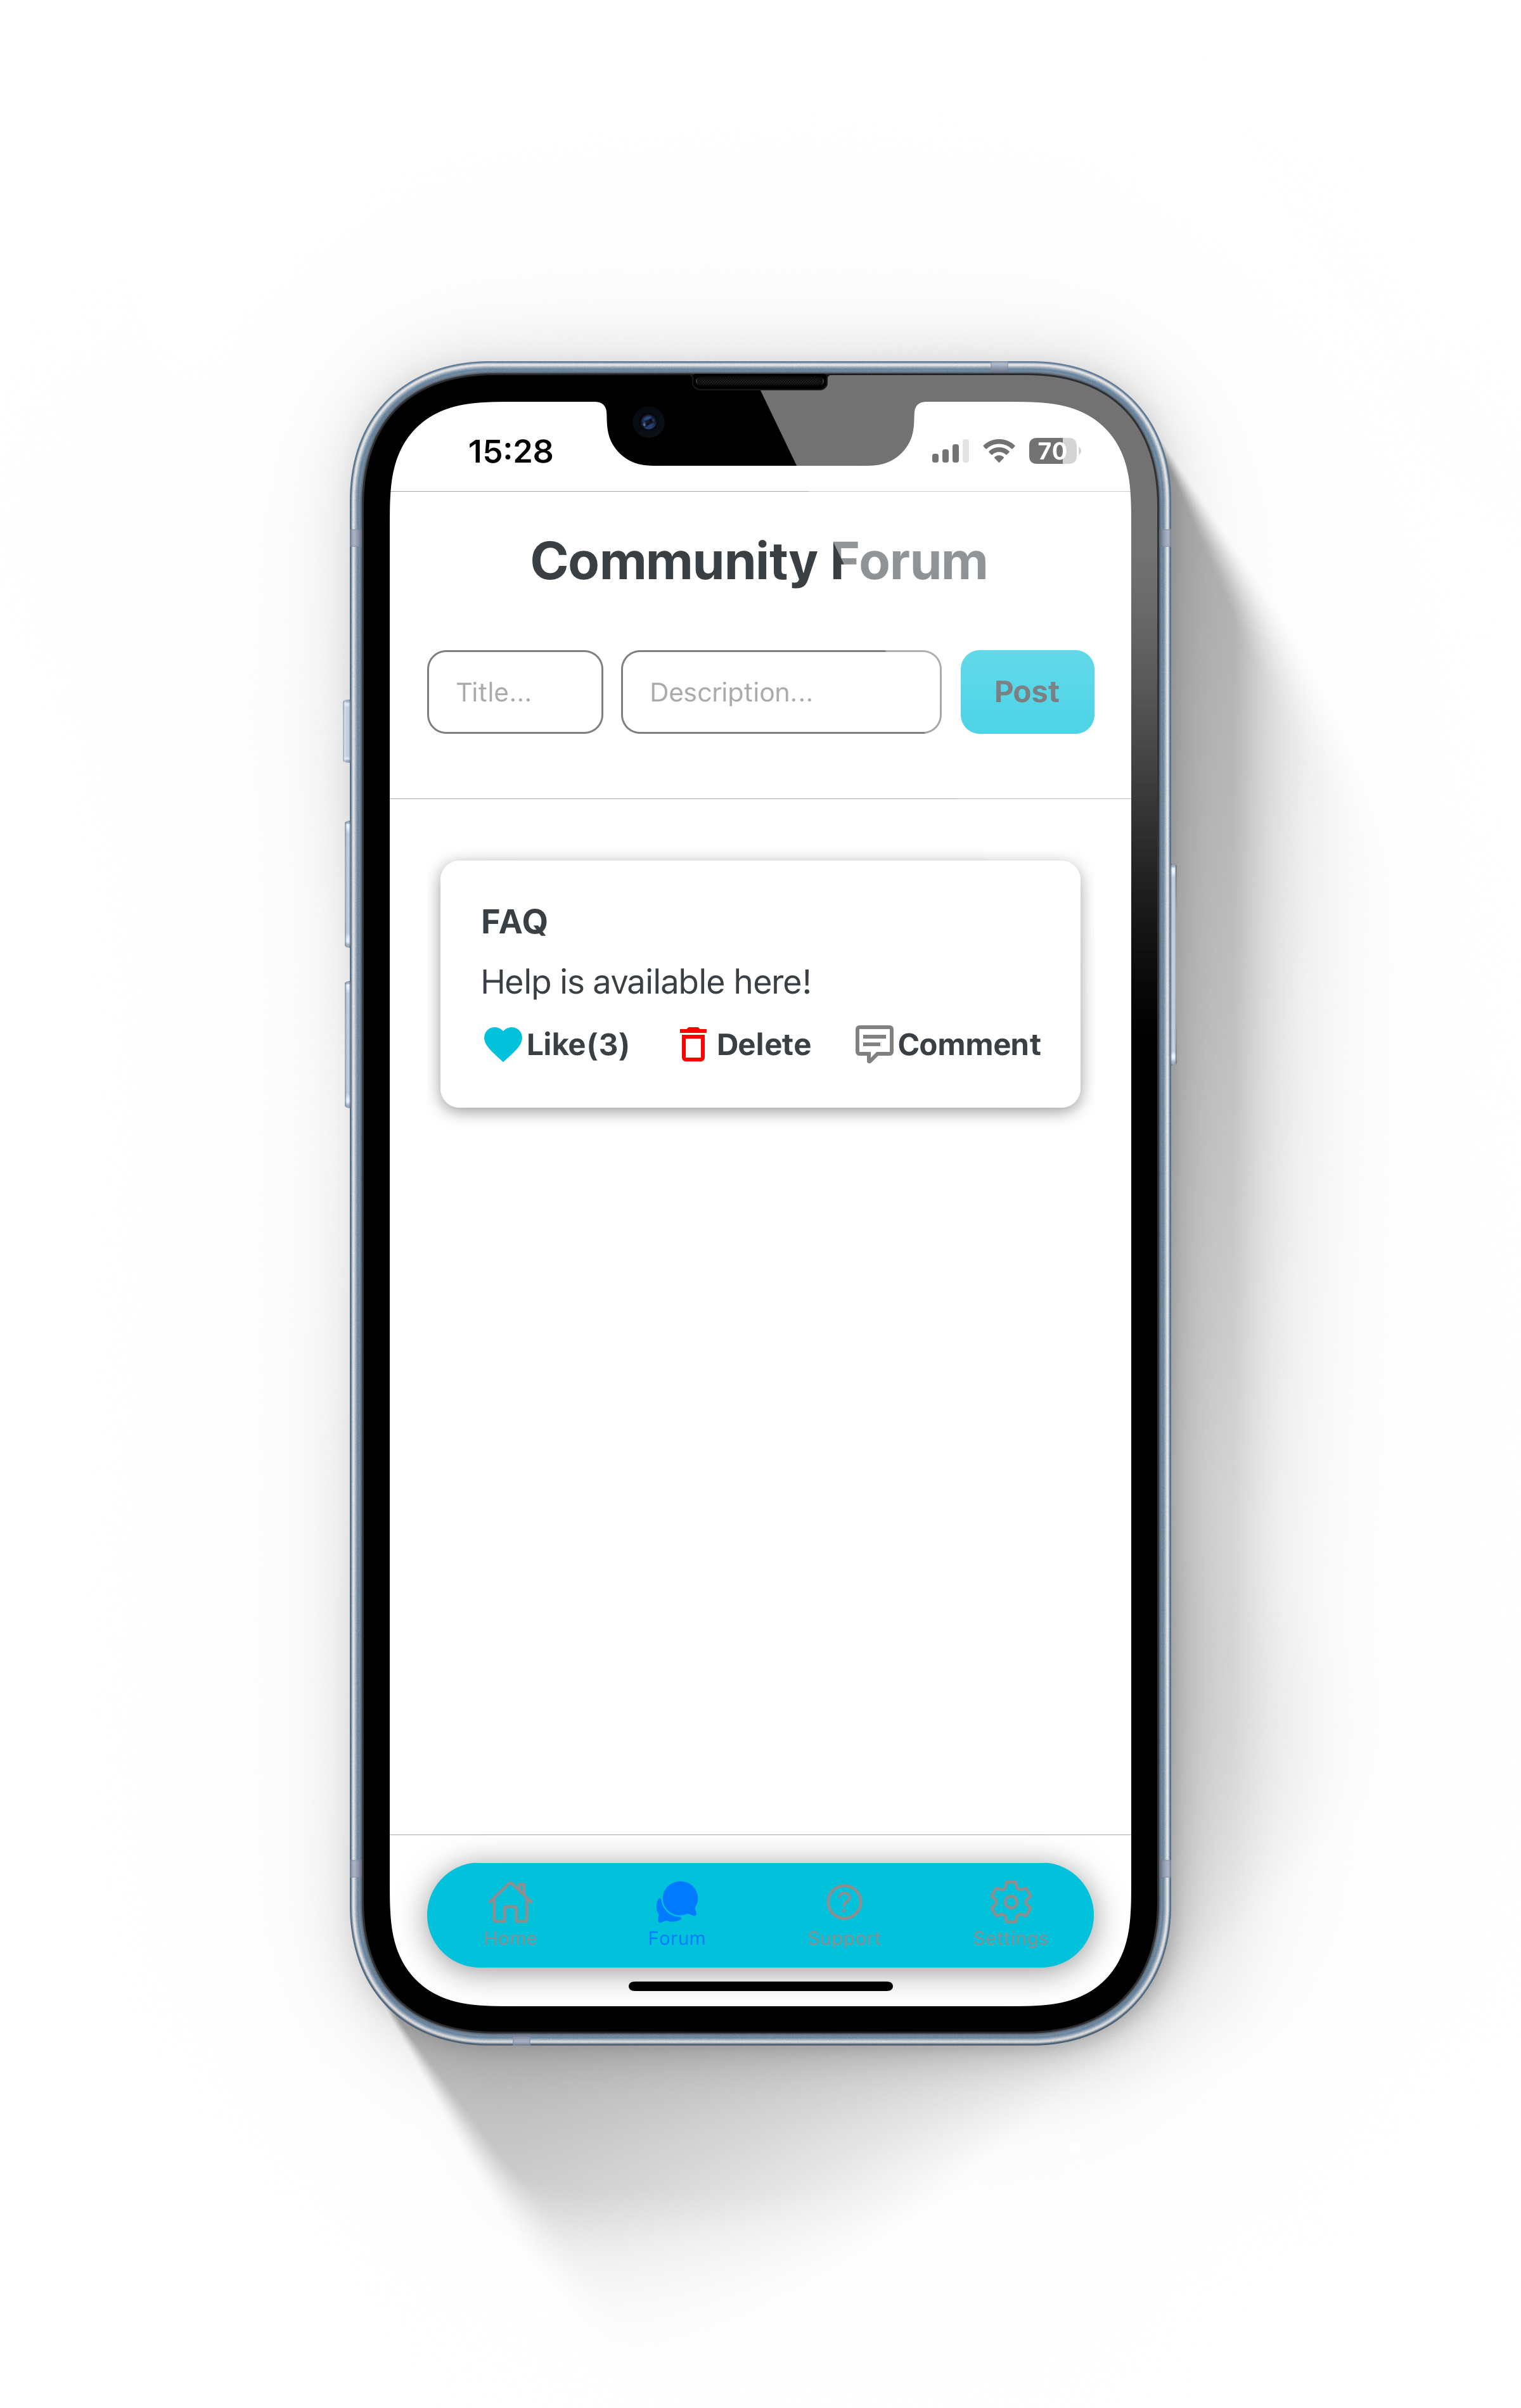
\includegraphics[width=0.5\textwidth]
    {LATEX/Appendices/Images/Software/Frontend/forum_screen.png}
    \caption{Forum Screen Appearance}
    \label{fig:forum screen}
\end{figure} 

The \textit{ForumScreen} is a functional component that takes \textit{navigation} as a prop. Post management features and state variables are provided by the \textit{useForumScreen} hook.

\begin{itemize}
    \item \textbf{Loading State:}
    \begin{itemize}
        \item If the \textit{loading} state is true, a loading message is displayed.
    \end{itemize}

    \item \textbf{Rendering Posts:}
    \begin{itemize}
        \item The \textit{renderPost} function handles posts rendering.
        \item The title and description of each post are shown within a card container.
        \item Posts include:
        \begin{itemize}
            \item The like button, which toggles the post's like state and updates the like count.
            \item The delete button, which is only shown if the user is the author of the post, allowing them to delete it.
            \item The comment button, which navigates the user to the comment screen for the post.
        \end{itemize}
    \end{itemize}

    \item \textbf{Return Statement:}
    \begin{itemize}
        \item The component returns a \textit{View} container with the following elements:
        \begin{itemize}
            \item A header text displaying \textit{``Community Forum''}.
            \item Input fields and a button for creating a new post.
            \begin{itemize}
                \item \textit{TextInput} fields for the post title and description.
                \item A \textit{TouchableOpacity} button for submitting the new post.
            \end{itemize}
            \item A separator line.
            \item A \textit{FlatList} component for displaying the list of posts.
            \begin{itemize}
                \item The \textit{FlatList} uses the \textit{renderPost} function to render each item.
                \item A footer component with padding is added to the end of the list.
            \end{itemize}
            \item Another separator line at the bottom.
        \end{itemize}
    \end{itemize}
\end{itemize}

\subsubsection{PostLoginScreens: UseForumScreen.js}

The \texttt{UseForumScreen.js} file defines a custom hook, \textit{useForumScreen}, and a context provider, \textit{PostProvider}, which manage the state and functionality of the forum screen.

\begin{itemize}
    \item \textbf{Context Creation:}
    \begin{itemize}
        \item \textit{PostContext}: Creates a context for managing and accessing forum-related state and functions.
        \item \textit{useForumScreen}: A custom hook that allows components to consume the \textit{PostContext}.
    \end{itemize}

    \item \textbf{State Variables:}
    \begin{itemize}
        \item \textit{posts}: An array to store the list of posts.
        \item \textit{loading}: A boolean flag to indicate if the posts are being fetched.
        \item \textit{newPostTitle}: A string to store the title of a new post.
        \item \textit{newPostDescription}: A string to store the description of a new post.
    \end{itemize}

    \item \textbf{useEffect Hook for Fetching Posts:}
    \begin{itemize}
        \item The \textit{useEffect} hook calls \textit{fetchPosts} to load the list of posts when the component mounts.
    \end{itemize}

    \item \textbf{Fetching Posts:}
    \begin{itemize}
        \item \textit{fetchPosts} is an asynchronous function.
        \begin{itemize}
            \item It sets \textit{loading} to \textit{true} before making the request.
            \item Retrieves the authentication token from \textit{SecureStore}.
            \item Makes a \textit{GET} request to the backend to fetch the posts.
            \item Sorts the posts by \textit{like\_count} in descending order.
            \item Updates the \textit{posts} state with the sorted posts and sets \textit{loading} to \textit{false}.
            \item Logs any errors encountered during the fetch.
        \end{itemize}
    \end{itemize}

    \item \textbf{Creating a Post:}
    \begin{itemize}
        \item \texttt{createPost} is an asynchronous function.
        \begin{itemize}
            \item it validates that the title and description are not empty.
            \item Resets the \textit{newPostTitle} and \textit{newPostDescription} states after validation.
            \item Makes a \textit{POST} request to the backend with the new post's title and description.
            \item If the request is successful, it adds the new post to the \textit{posts} state using \textit{LayoutAnimation} for a smooth transition.
            \item Logs any errors encountered during the post creation.
        \end{itemize}
    \end{itemize}

    \item \textbf{Liking a Post:}
    \begin{itemize}
        \item \texttt{handleLikePost} is an asynchronous function to like or unlike a post.
        \begin{itemize}
            \item Updates the local \textit{posts} state optimistically to reflect the like or unlike action immediately.
            \item Makes a \textit{POST} or \textit{DELETE} request to the backend based on whether the post is liked or unliked.
            \item If the request fails, reverts the optimistic update.
            \item Logs any errors encountered during the like or unlike action.
        \end{itemize}
    \end{itemize}

    \item \textbf{Deleting a Post:}
    \begin{itemize}
        \item \texttt{handleDeletePost} is an asynchronous function to delete a post.
        \begin{itemize}
            \item Makes a \textit{DELETE} request to the backend to delete the post.
            \item If the request is successful, removes the post from the \texttt{posts} state using \textit{LayoutAnimation} for a smooth transition.
            \item Logs any errors encountered during the post deletion.
        \end{itemize}
    \end{itemize}

    \item \textbf{Context Provider:}
    \begin{itemize}
        \item \texttt{PostProvider} wraps its children with \textit{PostContext.Provider} and provides the state variables and functions for managing posts.
        \item The provider value includes \textit{posts}, \textit{loading}, \textit{createPost}, \textit{handleLikePost}, \textit{handleDeletePost}, \textit{newPostTitle}, \textit{setNewPostTitle}, \textit{newPostDescription}, and \textit{setNewPostDescription}.
    \end{itemize}
\end{itemize}

\subsubsection{PostLoginScreens: CommentScreen.js}

\begin{figure}[!ht]
    \centering
    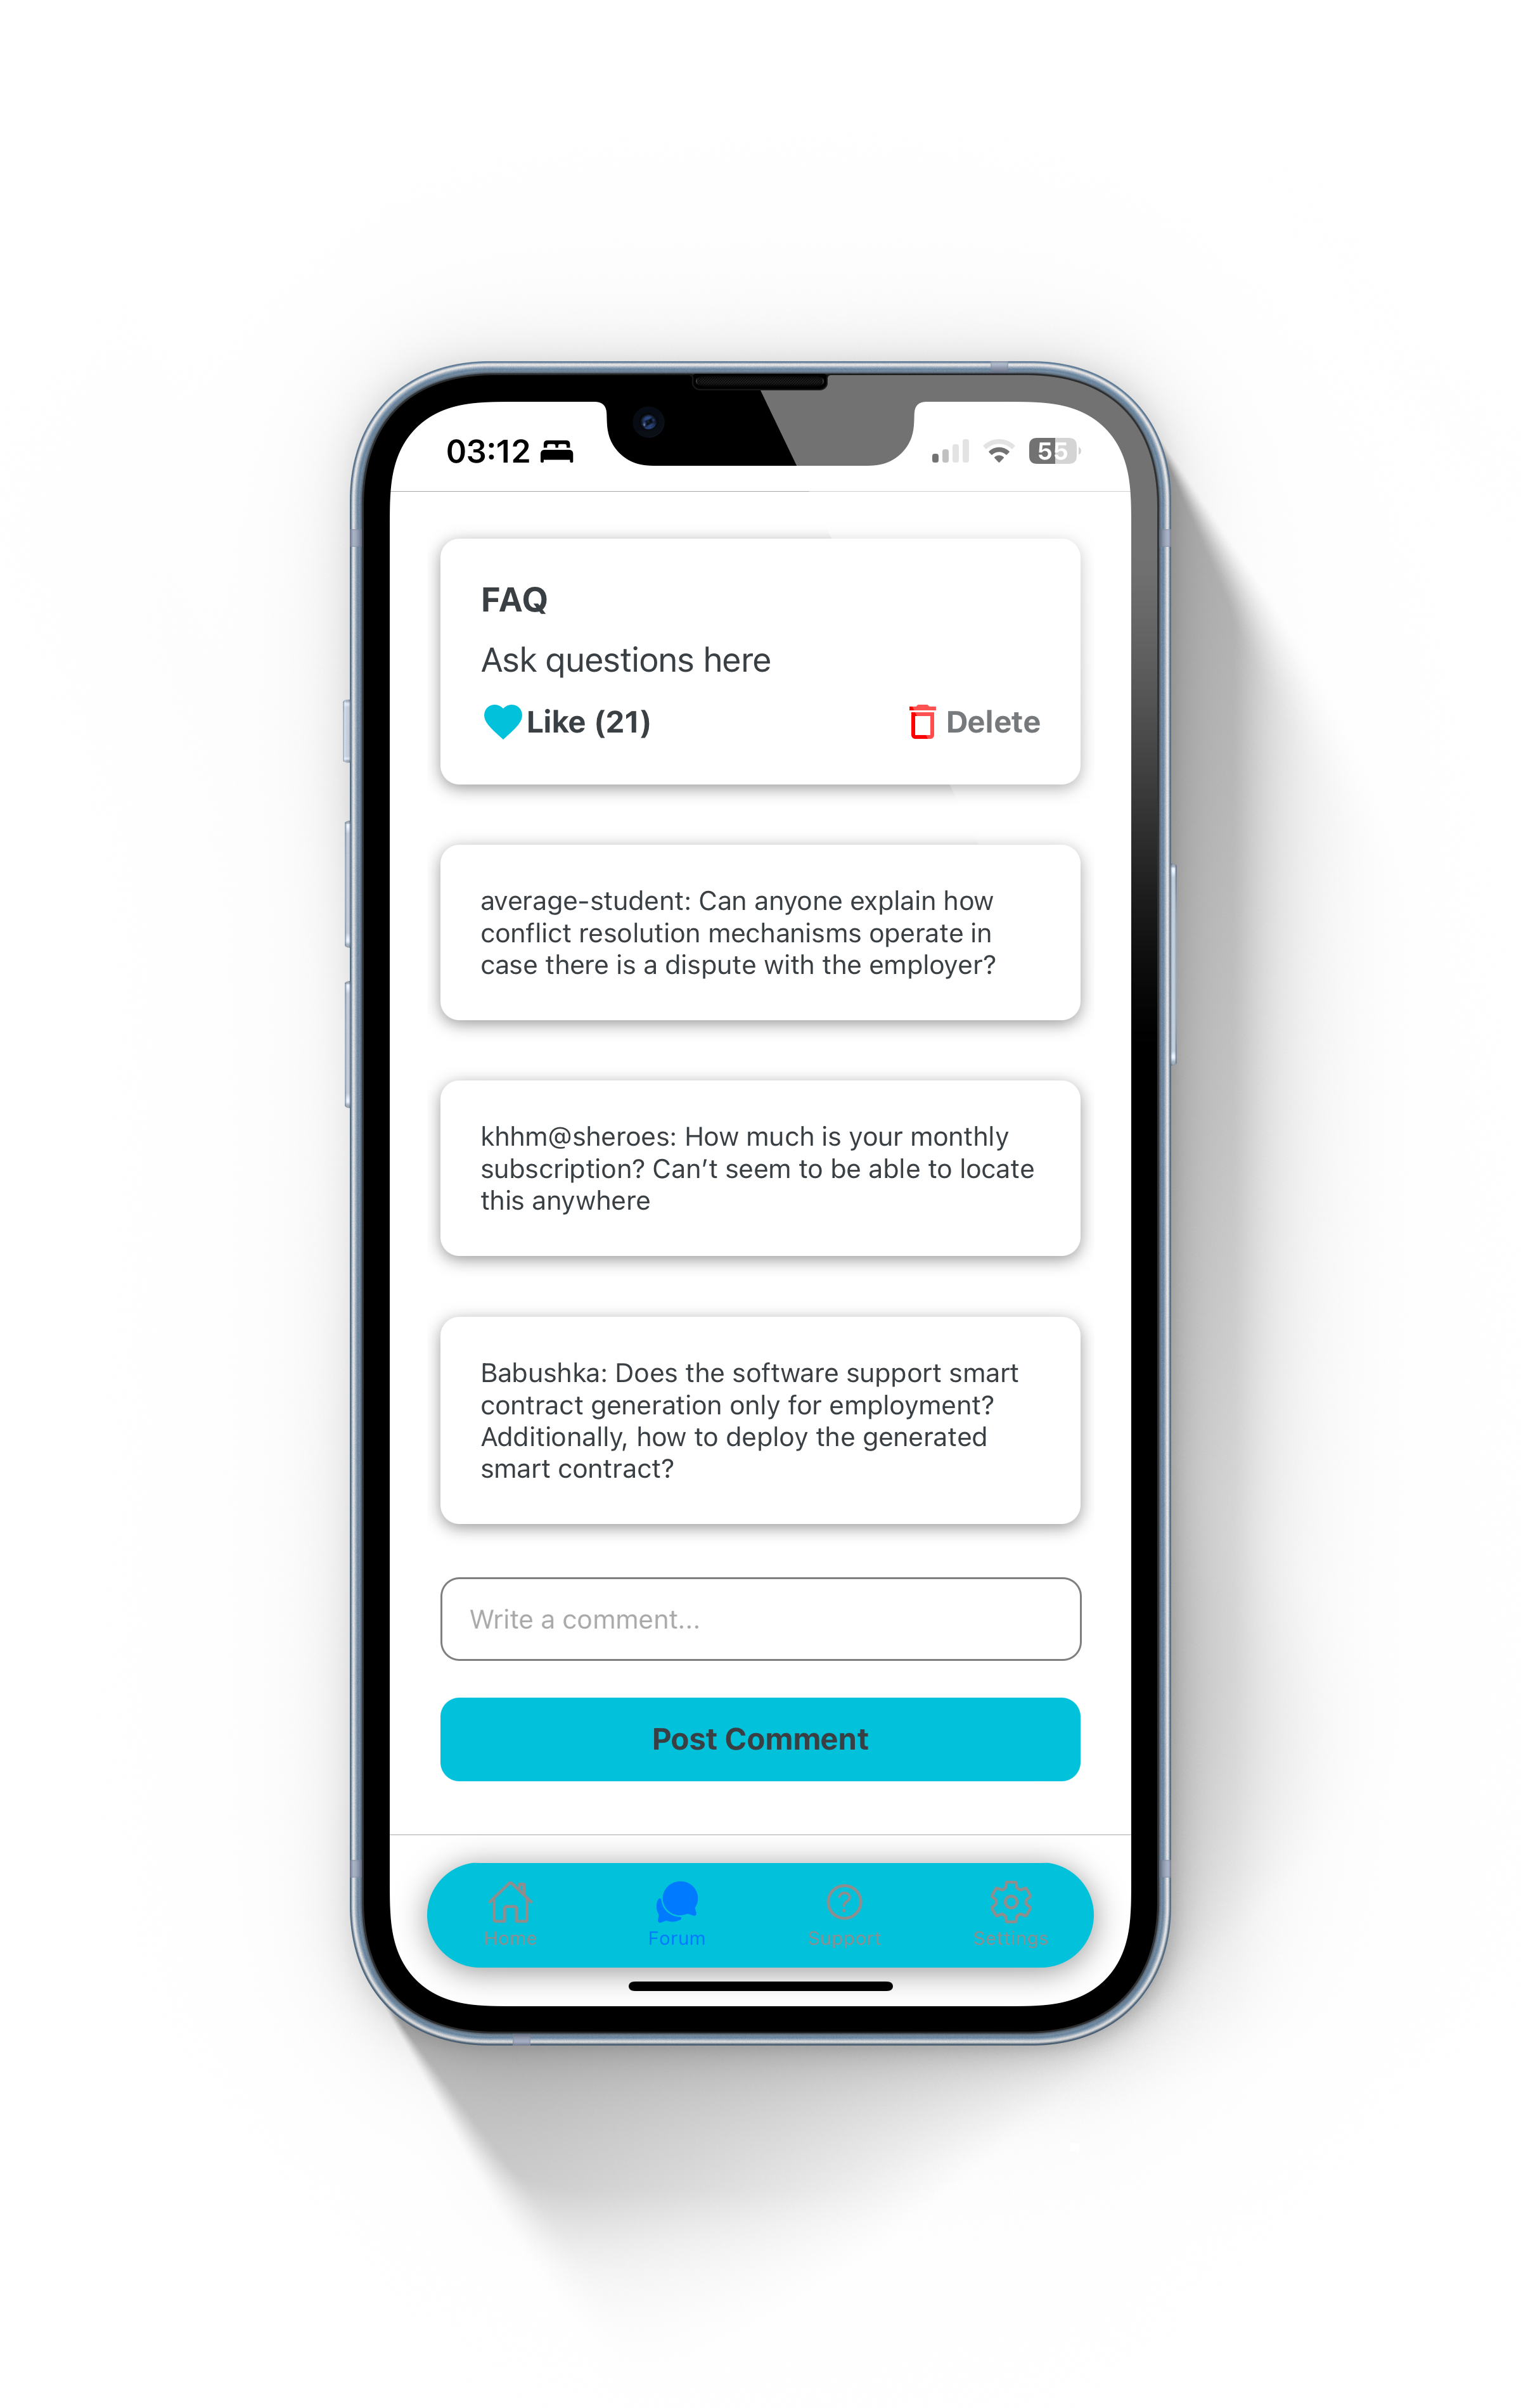
\includegraphics[width=0.5\textwidth]
    {LATEX/Appendices/Images/Software/Frontend/comment_screen.png}
    \caption{Comment Screen Appearance}
    \label{fig:comment screen}
\end{figure}

The \texttt{CommentScreen} component is defined as a functional component that takes \textit{route} and \textit{navigation} as props.

\begin{itemize}
    \item \textbf{Refs and Parameters:}
    \begin{itemize}
        \item The \textit{postId} is retrieved from \textit{route.params}.
        \item The post details are obtained from the \textit{posts} array using \textit{useForumScreen}.
    \end{itemize}

    \item \textbf{Fetching Comments:}
    \begin{itemize}
        \item When the component mounts, the first \textit{useEffect} is called to fetch comments for the post.
        \item Another \textit{useEffect} checks whether the post still exists in the \textit{posts} array. If the post has been deleted during user interactions on this screen, it navigates back to the forum screen.
    \end{itemize}

    \item \textbf{Return Statement:}
    \begin{itemize}
        \item The component returns a \textit{View} container with the following elements:
        \begin{itemize}
            \item A \textit{FlatList} component for displaying the list of comments.
            \begin{itemize}
                \item The list header displays the post title, description, and action buttons (like and delete).
                \item The \textit{renderItem} function renders each comment within a card container.
                \item The list footer includes an input field and a button for adding new comments.
            \end{itemize}
            \item A separator line at the bottom, positioned based on the keyboard height.
        \end{itemize}
    \end{itemize}
\end{itemize}

\subsubsection{PostLoginScreens: UseCommentScreen.js}

The \texttt{UseCommentScreen.js} file defines a custom hook that manages the state and functionality of the comments screen.

\begin{itemize}
    \item \textbf{State Variables:}
    \begin{itemize}
        \item \texttt{comments}: An array to store the list of comments for the post.
        \item \texttt{newComment}: A string to store the content of a new comment.
    \end{itemize}

    \item \textbf{useEffect Hook for Fetching Comments:}
    \begin{itemize}
        \item The \texttt{useEffect} hook calls \texttt{fetchComments} to load the list of comments when the component mounts, updates, or when the post ID changes.
    \end{itemize}

    \item \textbf{Fetching Comments:}
    \begin{itemize}
        \item \texttt{fetchComments} is an asynchronous function.
        \begin{itemize}
            \item It makes a \texttt{GET} request to the backend to fetch the comments for the specified post.
            \item Updates the \texttt{comments} state with the fetched comments.
            \item Logs any errors encountered during the fetch.
        \end{itemize}
    \end{itemize}

    \item \textbf{Adding a Comment:}
    \begin{itemize}
        \item \texttt{handleAddComment} is an asynchronous function.
        \begin{itemize}
            \item It makes a \texttt{POST} request to the backend with the content of the new comment.
            \item If the request is successful, fetches the updated list of comments and updates the \texttt{comments} state using \texttt{LayoutAnimation} for a smooth transition.
            \item Logs any errors encountered during the comment addition.
        \end{itemize}
    \end{itemize}

    \item \textbf{Return Values:}
    \begin{itemize}
        \item The hook returns the \texttt{comments} array, \texttt{newComment} state, \texttt{setNewComment} function, \texttt{fetchComments} function, and \texttt{handleAddComment} function, which are used by the \texttt{CommentScreen} component to manage and display comments.
    \end{itemize}
\end{itemize}

\subsubsection{PostLoginScreens: SupportScreen.js}

\begin{figure}[!ht]
    \centering
    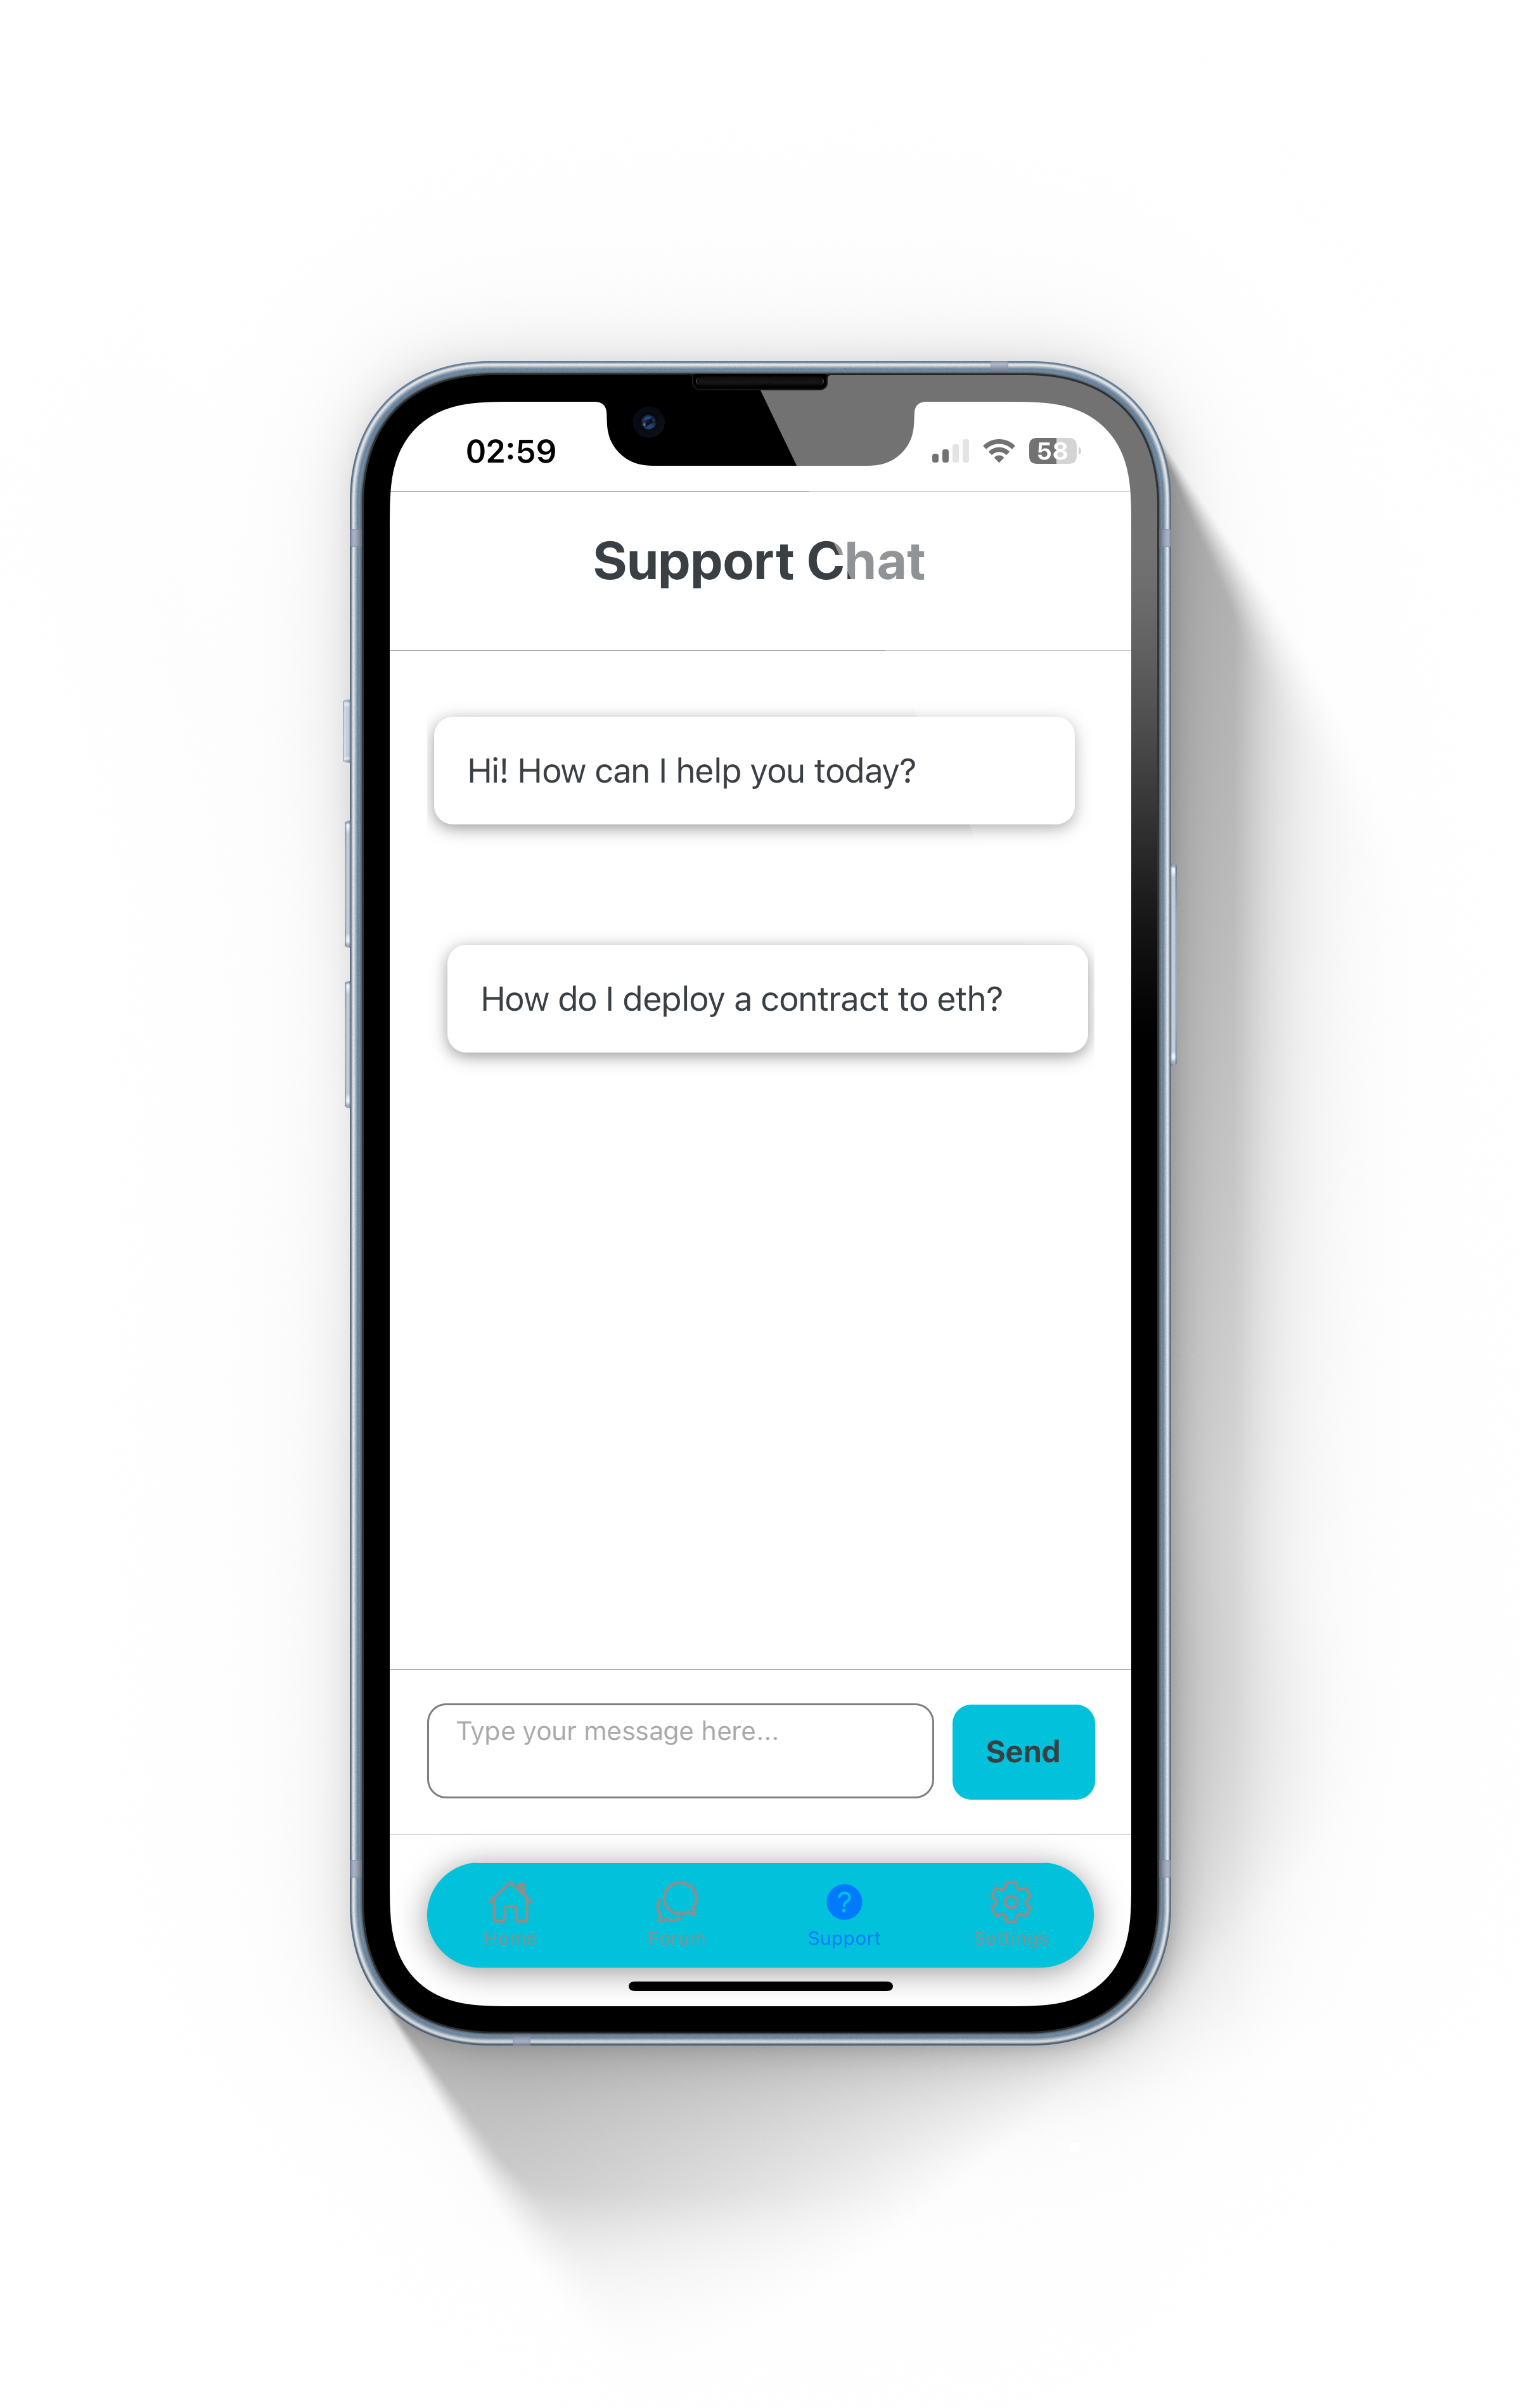
\includegraphics[width=0.5\textwidth]
    {LATEX/Appendices/Images/Software/Frontend/support_screen.png}
    \caption{Support Screen Appearance}
    \label{fig:support screen}
\end{figure}

The \texttt{SupportScreen.js} file defines a component responsible for providing a chat interface where users can interact with support agents.

\begin{itemize}
    \item \textbf{State Variables:}
    \begin{itemize}
        \item \textit{message}: A string to store the current user input message.
        \item \textit{messages}: An array to store the chat messages, initialised with a greeting message from the assistant.
    \end{itemize}

    \item \textbf{Sending Messages:}
    \begin{itemize}
        \item \textit{handleSendMessage} handles sending a message when the user presses the \textit{``send''} button.
        \begin{itemize}
            \item If the message is not empty, a new object is created with the user's input.
            \item The new message is added to the \textit{messages} array, and the input field is cleared.
        \end{itemize}
    \end{itemize}

    \item \textbf{Return Statement:}
    \begin{itemize}
        \item The component returns a \textit{View} container with the following elements:
        \begin{itemize}
            \item A header text displaying \textit{``Support Chat''}.
            \item A \textit{ScrollView} component to display the list of messages.
            \begin{itemize}
                \item Each message is rendered as a \textit{View} containing a \textit{Text} component with the message content.
                \item The message bubbles are styled differently based on whether the message is from an assistant or a user.
            \end{itemize}
            \item An input area at the bottom for the user to type and send messages.
            \begin{itemize}
                \item A \textit{TextInput} component for the user to type their message.
                \item A \textit{TouchableOpacity} button to send the message.
            \end{itemize}
            \item Multiple separator lines are included to enhance the visual layout.
        \end{itemize}
    \end{itemize}
\end{itemize}

Initially, it was planned to fine-tune another AI model to answer queries related to Solidity, smart contracts, and blockchain. However, due to time constraints, the AI model for this functionality was not developed. Additionally, the backend is not implemented to respond to these queries, resulting in a partially empty implementation. This functionality can be easily extended in future work.

\subsubsection{PostLoginScreens: SettingsScreen.js}

\begin{figure}[!ht]
    \centering
    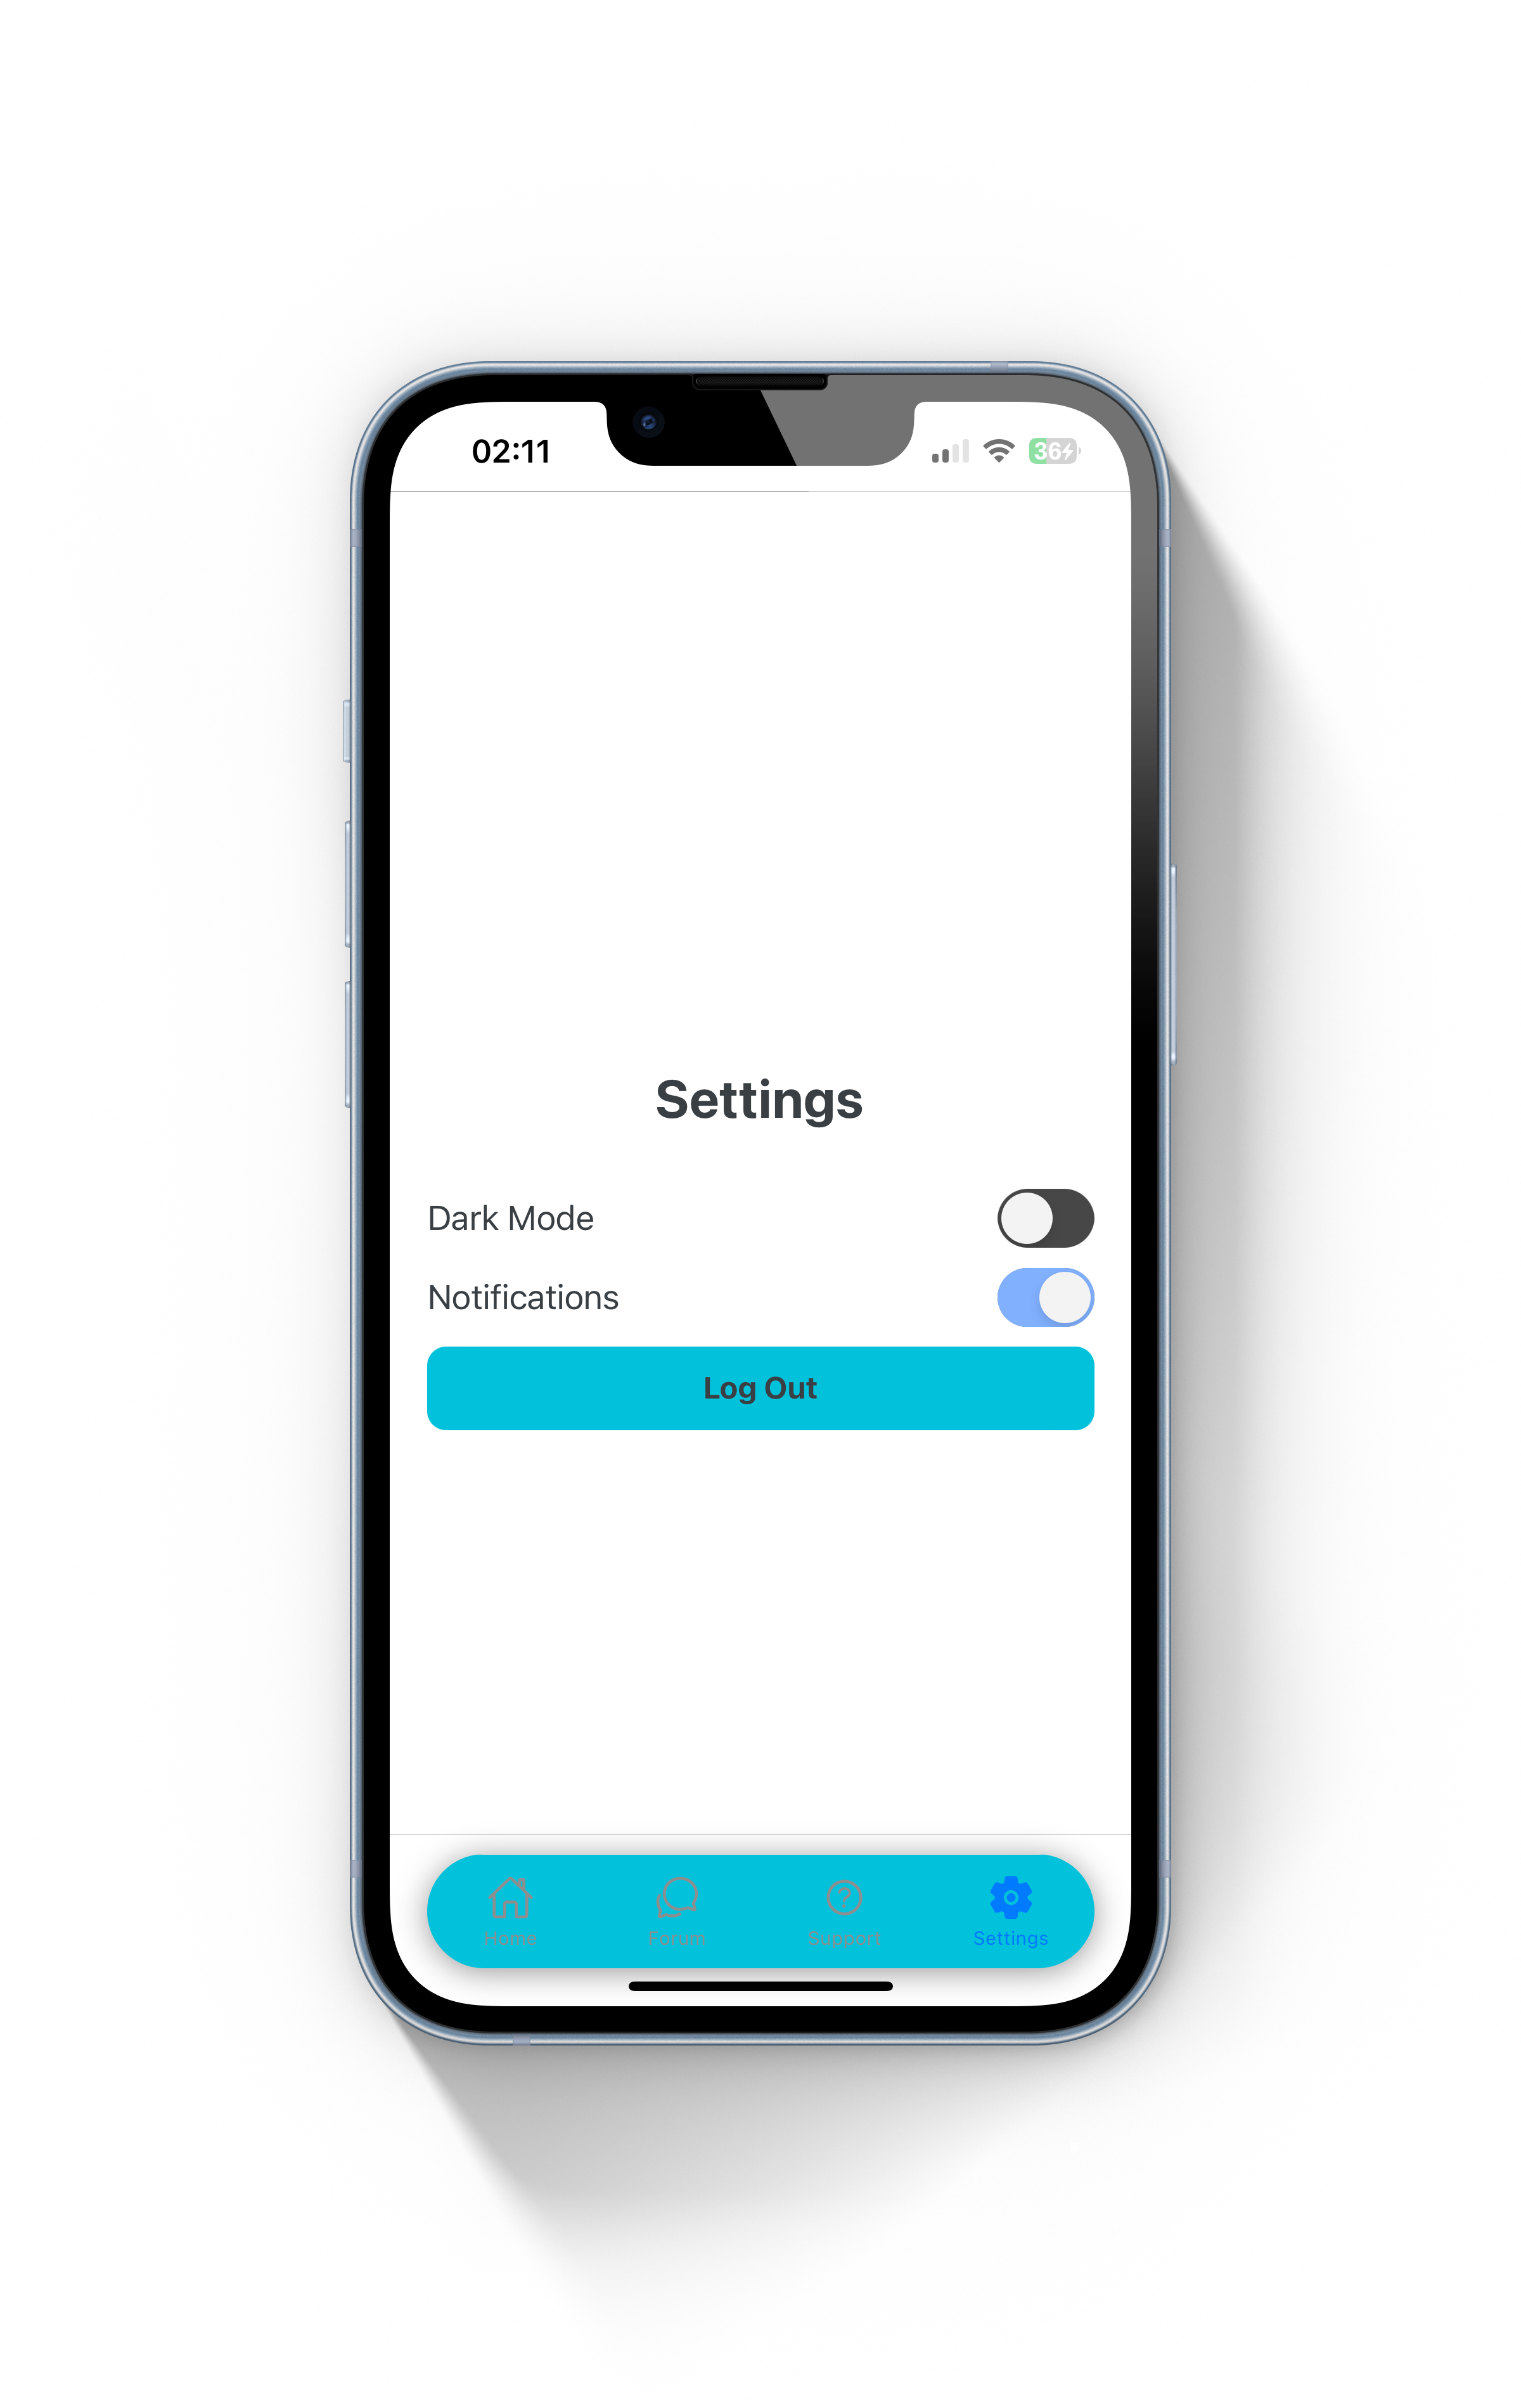
\includegraphics[width=0.5\textwidth]{LATEX/Appendices/Images/Software/Frontend/settings_screen.png}
    \caption{Settings Screen Appearance}
    \label{fig:settings screen}
\end{figure}

The \texttt{SettingsScreen.js} file defines a component responsible for providing a UI for adjusting application settings.

\begin{itemize}
    \item \textbf{Authentication and Notifications:}
    \begin{itemize}
        \item The \textit{handleLogout} function is obtained from \textit{AuthContext}.
        \item The \textit{notificationsEnabled}, \textit{setNotificationsEnabled}, and \textit{toggleNotifications} are obtained from and managed by \textit{useSettingsScreen}.
    \end{itemize}

    \item \textbf{Return Statement:}
    \begin{itemize}
        \item The component returns a \textit{View} container with the following elements:
        \begin{itemize}
            \item A header text displaying \textit{``Settings''}.
            \item A row container for toggling dark mode with \textit{Text} and \textit{Switch} components.
            \begin{itemize}
                \item The \textit{Switch} component toggles the \textit{isDarkMode} state using \textit{toggleTheme}.
            \end{itemize}
            \item A row container for toggling notifications with \textit{Text} and \textit{Switch} components.
            \begin{itemize}
                \item The \textit{Switch} component toggles the \textit{notificationsEnabled} state using \textit{toggleNotifications}.
            \end{itemize}
            \item A \textit{TouchableOpacity} button for logging out the user.
            \begin{itemize}
                \item This button triggers the \textit{handleLogout} function.
            \end{itemize}
            \item A separator line at the bottom for visual separation.
        \end{itemize}
    \end{itemize}
\end{itemize}

\subsubsection{PostLoginScreens: UseSettingsScreen.js}

The \texttt{UseSettingsScreen.js} file defines a custom hook that manages the state and functionality of the settings screen.

\begin{itemize}
    \item \textbf{State Variables:}
    \begin{itemize}
        \item \textit{notificationsEnabled}: A boolean state variable to indicate whether notifications are enabled or disabled.
    \end{itemize}

    \item \textbf{useEffect Hook for Checking Notification Token:}
    \begin{itemize}
        \item The \textit{useEffect} hook runs a function \textit{checkNotificationToken} when the component mounts.
        \item \textit{checkNotificationToken} is an asynchronous function.
        \begin{itemize}
            \item It retrieves the token using \textit{SecureStore.getItemAsync}.
            \item Updates the \textit{notificationsEnabled} state to \textit{true} if a token is found, otherwise sets it to \textit{false}.
        \end{itemize}
    \end{itemize}

    \item \textbf{Toggling Notifications:}
    \begin{itemize}
        \item \textit{toggleNotifications} is an asynchronous function.
        \begin{itemize}
            \item It calculates and updates the notification status by negating the current \textit{notificationsEnabled} state.
            \item If notifications are being enabled, it calls \textit{savePushToken}.
            \item Otherwise, it calls \textit{deletePushToken}.
        \end{itemize}
    \end{itemize}

    \item \textbf{Return Values:}
    \begin{itemize}
        \item The hook returns the \textit{notificationsEnabled} state, \textit{setNotificationsEnabled} function, and \textit{toggleNotifications} function, which are used by the \textit{SettingsScreen} component to manage notification settings.
    \end{itemize}
\end{itemize}

\subsection{Cross-Platform Fixes}

To be written soon...
